\documentclass[letterpaper,12pt,oneside,final]{book}
%%
%%  Gabarit de mémoire de maîtrise ou thèse de doctorat.
%%  Template for dissertations and theses @ Polytechnique Montreal.

%%  Normalement, il n'est pas nécessaire de modifier ce document
%%  sauf pour établir le langage (français ou anglais) et pour changer les noms des 
%%  fichiers à inclure.
%%  Usually, this document needs to be modified only to set up the language (French or English) 
%%  and to change the names of the files to include.
%%
%%  Version: 2018-07-31
%%
%%  Accepte les caractères accentués dans le document (UTF-8).


\makeatletter
\def\bstctlcite{\@ifnextchar[{\@bstctlcite}{\@bstctlcite[@auxout]}}
\def\@bstctlcite[#1]#2{\@bsphack
 \@for\@citeb:=#2\do{%
   \edef\@citeb{\expandafter\@firstofone\@citeb}%
   \if@filesw\immediate\write\csname #1\endcsname{\string\citation{\@citeb}}\fi}%
 \@esphack}
\makeatother

% LA COMMANDE SUIVANTE ÉTABLIT LE LANGAGE DE LA THÈSE : ÉCRIRE french POUR UNE THÈSE EN FRANÇAIS
% THE NEXT COMMAND DETERMINES THE LANGUAGE OF THE THESIS: WRITE english FOR A THESIS IN ENGLISH
\newcommand\Langue{french}            

\usepackage{ifthen}
\usepackage[utf8]{inputenc}
%%
%% Support pour l'anglais et le français (français par défaut).
%\usepackage[cyr]{aeguill}
\usepackage{lmodern}      % Police de caractères plus complète et généralement indistinguable visuellement de la police standard de LaTeX (Computer Modern).
\usepackage[T1]{fontenc}  % Bon encodage des caractères pour qu'Acrobat Reader reconnaisse les accents et les ligatures telles que ffi.

% le langage par défaut est le dernier de la liste, c'est-à-dire français
\ifthenelse{\equal{\Langue}{english}}{
	\usepackage[french,english]{babel}
}{
	\usepackage[english,french]{babel} 
}

%%
%% Charge le module d'affichage graphique.
\usepackage{graphicx}
\usepackage{epstopdf}  % Permet d'utiliser des .eps avec pdfLaTeX.
%%
%% Recherche des images dans les répertoires.
\graphicspath{{./images/}{./dia/}{./gnuplot/}}
%%
%% Un float peut apparaître seulement après sa définition, jamais avant.
\usepackage{flafter,placeins}
%%
%% Utilisation de natbib pour les citations et la bibliographie.
%\usepackage{natbib}
%%
%% Autres packages.
\usepackage{amsmath,color,soulutf8,longtable,colortbl,setspace,xspace,url,pdflscape,cite}
%%
%% Support des acronymes.
\usepackage[nolist]{acronym}
\onehalfspacing                % Interligne 1.5.
%%
%% Définition d'un style de page avec seulement le numéro de page à
%% droite. On s'assure aussi que le style de page par défaut soit
%% d'afficher le numéro de page en haut à droite.
\usepackage{fancyhdr}
\fancypagestyle{pagenumber}{\fancyhf{}\fancyhead[R]{\thepage}}
\renewcommand\headrulewidth{0pt}
\makeatletter
\let\ps@plain=\ps@pagenumber
\makeatother
%%
%% Module qui permet la création des bookmarks dans un fichier PDF.
%\usepackage[dvipdfm]{hyperref}
\usepackage{hyperref}
\usepackage{caption}  % Hyperlien vers la figure plutôt que son titre.
\makeatletter
\providecommand*{\toclevel@compteur}{0}
\makeatother
%%
%% Définitions spécifiques au format de rédaction de Poly.
%% Here we define the Poly formatting.
\RequirePackage[\Langue]{MemoireThese}
%%
%% Définitions spécifiques à l'étudiant.
%% -----------------------------------
%% ---> À MODIFIER PAR L'ETUDIANT / TO BE MODIFIED BY THE STUDENT <---
%% -----------------------------------
%%
%% Commandes qui affichent le titre du document, le nom de l'auteur, etc.
\newcommand\monTitre{Roue Cyr en matériaux composites : enrichir le langage acrobatique et scénique d'une discipline de cirque}
\newcommand\monPrenom{Charlotte}
\newcommand\monNom{Dubost}
\newcommand\monDepartement{génie mécanique}  % Department
\newcommand\maDiscipline{Génie mécanique}
\newcommand\monDiplome{M}        % (M)aîtrise ou (D)octorat / (M)aster or Ph(D)
\newcommand\anneeDepot{2020}    % Year
\newcommand\moisDepot{Juillet}       % Month
\newcommand\monSexe{F}           % "M" ou "F" = Gender
\newcommand\PageGarde{N}         % "O" ou "N" = Yes or No
\newcommand\AnnexesPresentes{O}  % "O" ou "N". Indique si le document comprend des annexes. / If the thesis includes annexes = O or N = No.
\newcommand\mesMotsClef{Cirque,roue,cyr,composites,elasticité}
\usepackage{gensymb}
%%
%%  DEFINITION DU / OF JURY
%%
%%  Pour la définition du jury, les macros suivantes sont definies:
%%  \PresidentJury, \DirecteurRecherche, \CoDirecteurRecherche, \MembreJury, \MembreExterneJury
%%
%%  Toutes les macros prennent 3 paramètres: Sexe (M/F), Nom, Prénom
%%  All the macros have 3 parameters: Sex (M/F), Last name, First name
\newcommand\monJury{\PresidentJury{F}{Nom}{Prenom}\\
\DirecteurRecherche{M}{Gosselin}{Frédérick}\\
\CoDirecteurRecherche{F}{Ross}{Annie}\\
\CoDirecteurRecherche{M}{Therriault}{Daniel}\\
\MembreJury{M}{Nom}{Prénom}\\
\MembreExterneJury{M}{Nom}{Prénom}}


\ifthenelse{\equal{\monDiplome}{M}}{
\newcommand\monSujet{Mémoire de maîtrise}
\newcommand\monDipl{Maîtrise ès sciences appliquées}
}{
\newcommand\monSujet{Thèse de doctorat}
\newcommand\monDipl{Philosophi\ae{} Doctor}
}
%%
%% Informations qui sont stockées dans un fichier PDF.
\hypersetup{
  pdftitle={\monTitre},
  pdfsubject={\monSujet},
  pdfauthor={\monPrenom{} \monNom},
  pdfkeywords={\mesMotsClef},
  bookmarksnumbered,
  pdfstartview={FitV},
  hidelinks,
  linktoc=all
}
%%
%% Il y a un document par chapitre du mémoire.
%%
\begin{document}
\bstctlcite{IEEEexample:BSTcontrol}

%%
%% Page de titre du mémoire.
\frontmatter
% Compte optionellement la page de garde dans la pagination.
\ifthenelse{\equal{\PageGarde}{O}}{\addtocounter{page}{1}}{}
\thispagestyle{empty}%
\begin{center}%
\vspace*{\stretch{0.1}}
\textbf{POLYTECHNIQUE MONTRÉAL}\\
affiliée à l'Université de Montréal\\
\vspace*{\stretch{1}}
\textbf{\monTitre}\\
\vspace*{\stretch{1}}
\textbf{\MakeUppercase{\monPrenom~\monNom}}\\
Département de~{\monDepartement}\\
\vspace*{\stretch{1}}
\ifthenelse{\equal{\monDiplome}{M}}{Mémoire présenté}{Thèse présentée} en vue de l'obtention du diplôme de~\emph{\monDipl}\\
\maDiscipline\\
\vskip 0.4in
\moisDepot~\anneeDepot
\end{center}%
\vspace*{\stretch{1}}
\copyright~\monPrenom~\monNom, \anneeDepot.
%%
%% Identification des membres du jury.
%%
\newpage\thispagestyle{empty}%
\begin{center}%

\vspace*{\stretch{0.1}}
\textbf{POLYTECHNIQUE MONTRÉAL}\\
affiliée à l'Université de Montréal\\
\vspace*{\stretch{2}}
Ce\ifthenelse{\equal{\monDiplome}{M}}{~mémoire intitulé}{tte thèse intitulée} :\\
\vspace*{\stretch{1}}
\textbf{\monTitre}\\
\vspace*{\stretch{1}}
présenté\ifthenelse{\equal{\monDiplome}{M}}{}{e}
par~\textbf{\mbox{\monPrenom~\MakeUppercase{\monNom}}}\\
en vue de l'obtention du diplôme de~\emph{\mbox{\monDipl}}\\
a été dûment accepté\ifthenelse{\equal{\monDiplome}{M}}{}{e} par le jury d'examen constitué de :\end{center}
\vspace*{\stretch{2}}
\monJury
%%
\pagestyle{pagenumber}%
%% Dédicace
%%
%% La dédicace est un hommage que l'auteur souhaite
%% rendre à une ou plusieurs personnes de son choix.
%%
\ifthenelse{\equal{\Langue}{english}}{
	\chapter*{DEDICATION}\thispagestyle{headings}
	\addcontentsline{toc}{compteur}{DEDICATION}
}{
	\chapter*{DÉDICACE}\thispagestyle{headings}
	\addcontentsline{toc}{compteur}{DÉDICACE}
}

\begin{flushright}
  \itshape
  A ceux qui mettent leurs connaissances et compétences au service de l'art, et à ceux qui cherchent un moyen de le faire. 
  \ldots
\end{flushright}
          % Dédicace du document.
% Remerciements / Acknowledgements
%
%  Grâce aux remerciements, l'auteur attire l'attention du lecteur
% sur l'aide que certaines personnes lui ont apportée, sur leurs
% conseils ou sur toute autre forme de contribution lors de la
% réalisation de son mémoire. Le cas échéant, c'est dans cette section
% que le candidat doit témoigner sa reconnaissance à son directeur de
% recherche, aux organismes dispensateurs de subventions ou aux
% entreprises qui lui ont accordé des bourses ou des fonds de
% recherche.
\ifthenelse{\equal{\Langue}{english}}{
	\chapter*{ACKNOWLEDGEMENTS}\thispagestyle{headings}
	\addcontentsline{toc}{compteur}{ACKNOWLEDGEMENTS}
}{
	\chapter*{REMERCIEMENTS}\thispagestyle{headings}
	\addcontentsline{toc}{compteur}{REMERCIEMENTS}
}
%
Merci à mes directeurs de recherche, Frédérick Gosselin, Annie Ross et Daniel Therriault pour l'énergie et le temps qu'ils ont accordé à l'accompagnement de ce projet ainsi que pour leur vivacité d'esprit et l'excellence de leurs expertises dont j'ai eu la chance de bénéficier. \\\\
Merci à Marion Cossin pour son soutien, ses précieux conseils et son appui au sein de l'Ecole Nationale de Cirque de Montréal dès le début du projet.\\\\
Merci à toute l'équipe de l'Ecole Nationale de Cirque pour sa collaboration.
     % Remerciements.
% Résumé du mémoire.
%
\chapter*{RÉSUMÉ}\thispagestyle{headings}
\addcontentsline{toc}{compteur}{RÉSUMÉ}

La roue Cyr, agrès de cirque, est un anneau métallique à taille humaine. L’utilisateur s’y agrippe et exécute des figures acrobatiques en tournant. Le poids, la rigidité et la flexibilité de la roue sont donc des paramètres déterminants pour le mouvement de l’utilisateur. Depuis son invention, la roue Cyr a été revisitée par les artistes et les fabricants pour créer des agrès hybrides. Alors que le cirque s’approprie les matériaux composites utilisés pour l’équipement sportif, les adeptes de la roue Cyr se demandent ce qu’une roue plus légère et flexible apporterait à la discipline. Ces roues sont constituées de poutres courbes connectées par des manchons, ce qui implique des coûts de fabrication excluant la méthode ‘essai-erreur’ pour répondre à la question. Tous les projets alliant roue Cyr et matériaux composites restent ainsi inachevés. 

A ce jour la roue Cyr ne fait l’objet d’aucune publication scientifique. Cependant, son mouvement est similaire à celui du disque d’Euler : nous adapterons donc les modèles théoriques issus de la littérature comme base pour déterminer comment la géométrie de la roue Cyr influence sa stabilité dynamique. Nous étudions aussi le saut d’une roue comprimée puis relâchée, en référant aux travaux de Yang et Kim sur le stockage d’énergie élastique dans des anneaux.

La conception, la fabrication et les tests d’une roue Cyr en matériaux composites combine une expérience pratique de l’agrès, l’impression 3D de matériaux composites à grande échelle et la dynamique du disque d’Euler. L’issue de ces travaux contribuera à clarifier l’intérêt, pour les fabricants, d’investir dans les roues Cyr en composites.
Notre objectif est de déterminer les propriétés du matériau et la géométrie optimales pour la stabilité et le saut d’une roue Cyr, d’imprimer un prototype et de tester son potentiel acrobatique avec des artistes de cirque.
      % Résumé du sujet en français.
% Abstract
%
% Résumé de la recherche écrit en anglais sans être
% une traduction mot à mot du résumé écrit en français.

\chapter*{ABSTRACT}\thispagestyle{headings}
\addcontentsline{toc}{compteur}{ABSTRACT}
%

A Cyr wheel is a circus apparatus consisting of a human sized metallic ring. The user stands inside the wheel and performs acrobatic figures while spinning. The weight, rigidity and geometry of the wheel are thus determinant parameters for the user’s motion. Since it has been invented, the Cyr wheel has been revisited by circus artists and manufacturers to create hybrid apparatuses. As composite manufacturing for sports spreads to circus, Cyr wheel adepts wonder what a lighter, more flexible wheel would result in. These wheels are composed of curved beams connected by sleeves: this implies fabrication costs and excludes the ‘trial and error’ method to answer the question. Thus, no composite Cyr wheel project has been completed yet. 

To this day there isn’t any scientific publication specific to Cyr wheel. Nevertheless, its dynamics relate to Euler’s disk. We will adapt theoretical models in the literature as a basis to determine how the Cyr wheel geometry influences dynamic stability. We will also focus on the jump of a wheel being bent and released, and thus refer to Yang and Kim article about energy storage in elastic rings as a comparative study.

The design, manufacturing and test of a 3D printed composite Cyr Wheel prototype combines practical experience of the apparatus, familiarity with composite materials, large-scale 3D printing processes and dynamics of Euler’s disk-like motions. The outcome will shed light on the interests for manufacturers to invest in composite Cyr wheels. 
Our objective is to determine which mechanical properties and geometry will optimize the stability and jumps of a Cyr wheel, 3D print a prototype and test acrobatic possibilities with circus artists.
\\
          % Résumé du sujet en anglais.

{\setlength{\parskip}{0pt}
%%
%% Table des matières.
\ifthenelse{\equal{\Langue}{english}}{
	\renewcommand\contentsname{TABLE OF CONTENTS}
}{
	\renewcommand\contentsname{TABLE DES MATIÈRES}
}
\tableofcontents
%%
%% Liste des tableaux.
\ifthenelse{\equal{\Langue}{english}}{
	\renewcommand\listtablename{LIST OF TABLES}
}{
	\renewcommand\listtablename{LISTE DES TABLEAUX}
}\listoftables
%%
%% Table des figures.
\ifthenelse{\equal{\Langue}{english}}{
	\renewcommand\listfigurename{LIST OF FIGURES}
}{
	\renewcommand\listfigurename{LISTE DES FIGURES}
}\listoffigures
%%
%% Liste des annexes au besoin.
}

% Liste des sigles et abbréviations / List of acronyms and abbreviations
\ifthenelse{\equal{\Langue}{english}}{
	\newcommand\abbrevname{LIST OF SYMBOLS AND ACRONYMS}
}{
	\newcommand\abbrevname{LISTE DES SIGLES ET ABRÉVIATIONS}
}
\chapter*{\abbrevname}
\addcontentsline{toc}{compteur}{\abbrevname}
\pagestyle{pagenumber}
%
\begin{acronym}
  \acro{ENC}{Ecole Nationale de Cirque}
  \acro{CNAC}{Centre National des Arts du Cirque}
  \acro{FEDEC}{Fédération Européenne Des Ecoles de Cirque professionnelles}
\end{acronym}
%
\begin{longtable}{lp{5in}}
ENC       & Ecole Nationale de Cirque\\
CNAC       & Centre National des Arts du Cirque\\
FEDEC       & Fédération Européenne Des Ecoles de Cirque professionnelles\\
2DDL       & Deux degrés de liberté\\
PLA       & Acide polylactique\\
\end{longtable}

       % Liste des sigles et abréviations.
\ifthenelse{\equal{\AnnexesPresentes}{O}}{\listofappendices}{}
\mainmatter
% Dans l'introduction, on présente le problème étudié et les buts
% poursuivis. L'introduction permet de faire connaître le cadre de la
% recherche et d'en préciser le domaine d'application. Elle fournit
% les précisions nécessaires en ce qui concerne le contexte de
% réalisation de la recherche, l'approche envisagée, l'évolution de
% la réalisation. En fait, l'introduction présente au lecteur ce
% qu'il doit savoir pour comprendre la recherche et en connaître la
% portée.

\Chapter{INTRODUCTION}\label{sec:Introduction}  % 10-12 lignes pour introduire le sujet.

\\
Support d'acrobatie entraînant le corps de l'utilisateur dans un mouvement de rotation, mais pouvant aussi être manipulée par ce dernier, la roue Cyr se trouve à mi-chemin entre les disciplines acrobatique, d'équilibrisme et de manipulation d'objet. La réalisation de figures acrobatiques repose sur l'équilibre dynamique entre la roue et le corps de l'utilisateur. Ce dernier module le rythme et la force qu'il applique à la roue en fonction de sa masse, son inertie, sa géométrie. La popularité croissante des matériaux composites pour la fabrication d'équipement de cirque comme les mats ou les portiques éveille la curiosité de la communauté circassienne sur les possibilités nouvelles qu'une roue Cyr en composites apporterait. L'enjeu est double: le procédé de fabrication offrant un éventail de possibilités géométriques inaccessibles avec les métaux ainsi qu'un choix de propriétés mécaniques plus varié, c'est une opportunité d'optimiser des mouvements déjà existants mais aussi d'inventer de nouvelles figures avec une roue Cyr faite d'un matériau dont les propriétés élastiques permettent, par exemple, de sauter avec la roue.
%%
%%  CONCEPTS DE BASE / BASIC CONCEPTS
%%
\section{Définitions et concepts de base}  % environ 2-3 pages

\subsection{Définitions}
\paragraph{Circassien(ne):} relatif au cirque 
\paragraph{Agrès de cirque:} équipement nécessaire à la pratique d'une discipline circassienne. Exemples: la roue Cyr, le trapèze, le tissu aérien, les cannes d'équilibre, le mat chinois...
\paragraph{Disque d'Euler:} disque ayant un mouvement de rotation similaire à celui d'une pièce qu'on fait tourner sur une surface plane. Lorsque son mouvement entre en phase terminale sa vitesse de rotation augmente de façon impressionnante, ce qui lui a valu de devenir un jouet éducatif, mais aussi de faire l'objet de nombreuses publications scientifiques. Son mouvement est similaire à un des mouvements caractéristiques de la roue Cyr.


\subsection{Historique de la roue Cyr}
La roue Cyr que l'on retrouve dans les spectacles de cirque contemporains doit son  nom à Daniel Cyr, qui fabriqua sa première roue en 1996 \cite{Inertie}. A cette dernière, faite en une seule pièce d'acier recouverte d'un revêtement en PVC, succéda rapidement  une roue Cyr démontable en plusieurs parties. La première apparition marquante de la roue Cyr sur la scène circassienne eut lieu en 1998 dans un spectacle du Cirque Eloize, dont Daniel Cyr est le co-fondateur. Une médaille d'argent remportée en 2003 par ce dernier au Festival Mondial du Cirque de Demain acheva d'asseoir la popularité de ce nouvel agrès dans le secteur du cirque, mais également en tant que sport.\\
Cependant l'idée d'une roue à la géométrie torique dont le diamètre avoisine la taille humaine est bien antérieure à la création de Daniel Cyr \cite{Inertiehist,gymmedia,howstuffwork}. En effet, plusieurs agrès d'apparence similaire à celle de la roue Cyr sont apparus du côté de l'Allemagne dès le début du vingtième siècle. On remarquera en particulier l'Einrefen, inventé en 1930 par Adalbert von Rekowski, qui diffère de la roue Cyr par des poignées intérieures pour les mains et les pieds (figure \ref{fig:cyrhelga}). \\

\begin{figure}[h]
\centering
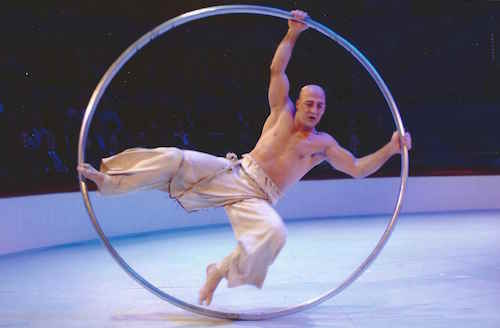
\includegraphics[width=200]{images_autres/danielcyr2003.jpeg}
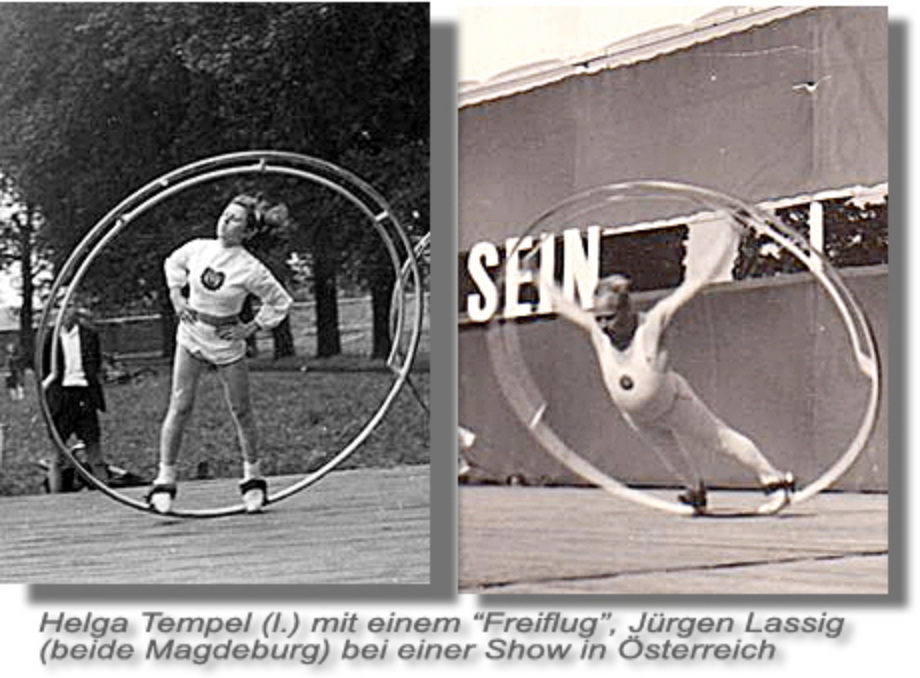
\includegraphics[width=200]{images_autres/helga1950.png}
\caption{Daniel Cyr au 24e festival mondial de demain en 2003 \cite{danielcyr} (gauche) et la gymnaste Helga Tempel sur l'Einrefen en 1950 \cite{gymmedia}) (droite).}
\label{fig:cyrhelga}
\end{figure}


Depuis, la roue Cyr continue d'évoluer, comme le montrent les agrès hybrides conçus en dérivant le concept de la roue Cyr pour créer de nouvelles possibilités acrobatiques (figure \ref{fig:cyrhyb}). Les procédés de fabrication se sont eux aussi affinés \cite{corbin}, et les roues Cyr lumineuses programmables ont vu le jour.\\
La fabrication en matériaux composites se présente aujourd'hui comme l'étape suivante dans l'évolution de l'agrès.

\begin{figure}[h]
\centering
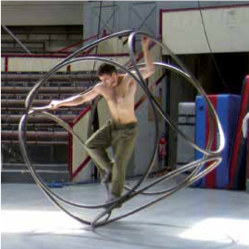
\includegraphics[width=120]{images_autres/hyb1.png}
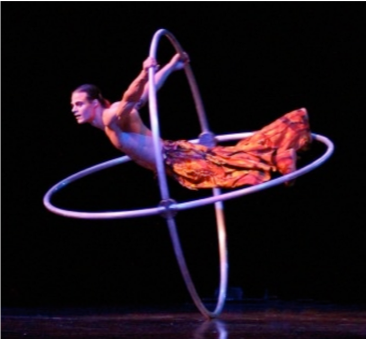
\includegraphics[width=130]{images_autres/hyb2.png}
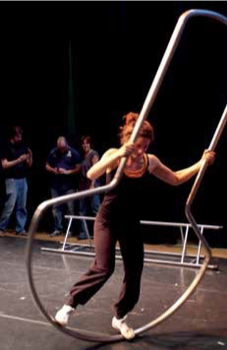
\includegraphics[width=80]{images_autres/hyb3.png}
\caption{Agrès de cirque dérivés de la roue Cyr \cite{Fedec2011}.}
\label{fig:cyrhyb}
\end{figure}

\subsection{Les figures de roue Cyr}
Nous présentons ici les figures de roue Cyr constituant la base principale de la discipline. Ces dernières, ainsi que d'autres figures plus avancées sont détaillées dans le manuel de la FEDEC \cite{Fedec2011}
\subsubsection{La valse (ou pas de base)}
Le corps est positionné de façon symétrique, avec bras et jambes chacun inclinés à 45\degree de la verticale. L'utilisateur initie la rotation d'une poussée du pied puis accompagne le mouvement de la roue en utilisant le transfert de son poids, tirant et poussant successivement la roue dans le sens de la rotation.\\
Ce mouvement se décline en plusieurs variations : par exemple un lâcher de pied, qui avec un arc de cercle de la jambe devient un arabesque. Il s'exécute aussi à une seule main, les mains croisées, en serrant et croisant les jambes ou en les écartant jusqu'au grand écart latéral. Il est aussi possible de placer un pied sur la roue au niveau de la tête, en grand écart facial. D'autres variantes jouent avec la position du corps : de profil, dans le plan de la roue, arqué vers l'intérieur, tendu vers l'extérieur...



\subsubsection{Les tours}
Dissociation du mouvement : la roue tourne mais pas le corps. Ce type de figure s'exécute en effectuant un demi-tour, un tour complet, ou même un tour en suspension avec l'utilisateur suspendu à la roue par une main.

\subsubsection{Les vrilles}
Dissociation inverse : le corps tourne dans le référentiel de la roue. De même ce type de figure se décline de la demi vrille à la vrille complète en suspension.

\subsubsection{Les suspensions}
Comme l'indique le nom, les pieds ne sont pas sur la roue. On peut par exemple exécuter la valse en suspension, sans les pieds, ou simplement prendre de l'élan puis lâcher les pieds et adopter une position groupée en tournant sur place, ce qui a pour effet d'augmenter la vitesse de rotation. Il est possible de se suspendre par une ou deux mains, par les coudes, les bras tendus ou fléchis. La suspension est la base de la figure du Superman: corps gainé, jambes tendues vers l'arrière.

\subsubsection{Le drapeau}
La roue n'est tenue que par la main et le pied d'un même côté. La rotation est alimentée en poussant et tirant avec la main et le pied restants, tout en tendant puis groupant successivement la main et le pied lâchés.

\subsubsection{Les sauts}
La roue tourne sur elle même, l'utilisateur saute et prend appui comme il le souhaite, bras tendus, pliés, ou même en position assise sur la roue. Il maintient sa position pour quelques tours et peut ensuite atterrir sur le sol ou directement sur la roue.

\subsubsection{Le corner ou inclinaison horizontale}
L'utilisateur se décale sur un côté de la roue jambes serrées, prend appui jambes fléchies puis plonge vers le sol, jambes tendues : le corps se retrouve en position horizontale pour un demi tour. Cette figure peut se réaliser en lâchant un bras, un pied, ou un bras et un pied simultanément.

\subsubsection{Le saut de mains}
L'utilisateur pousse la roue vers le sol avec une main, accompagne le renversement avec son poids, ouvre les doigts quand sa main arrive au niveau du sol puis la tire au dessus de sa tête et la pousse avec ses jambes afin de revenir à l'endroit. Cette figure s'exécute en avant, en arrière, en position de profil, à une jambe.

\subsubsection{La roue}
La roue roule sur sa tranche et l'utilisateur entretient le mouvement au moyen de transferts de poids. On peut enchaîner plusieurs roues le long d'une trajectoire circulaire ou rectiligne. Il est possible de la combiner avec d'autres figures ou changements de direction et d'enchaîner ainsi les roues dans des sens différents.

\subsubsection{La pièce}
Ce mouvement est semblable à la rotation d'une pièce de monnaie dans la phase terminale du mouvement. L'utilisateur, gainé, ouvre successivement les doigts pour ne pas les écraser lorsque ses mains arrivent au niveau du sol, et transfère son poids pour accompagner le mouvement et l'alimenter aussi longtemps qu'il le souhaite. Cette figure peut s'exécuter à différentes hauteurs du sol, plus la pièce est basse, plus la vitesse sera élevée. On peut aussi la réaliser à l'envers, le corps arqué (pièce dorsale).

\begin{figure}[h]
\centering
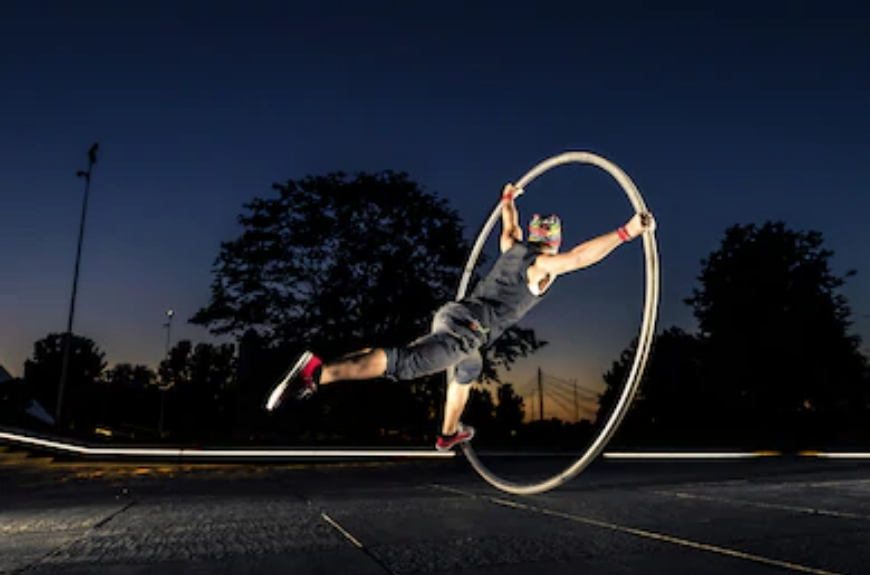
\includegraphics[width=200]{images_autres/valse.png}
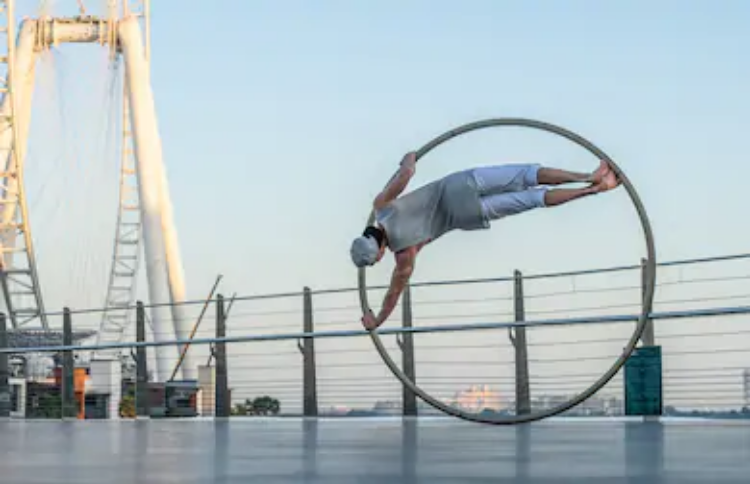
\includegraphics[width=210]{images_autres/corner.png}
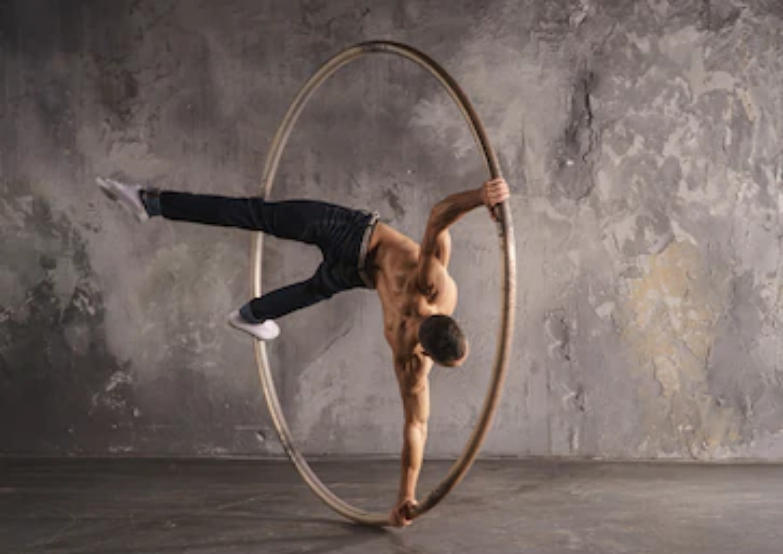
\includegraphics[width=200]{images_autres/handspring.png}
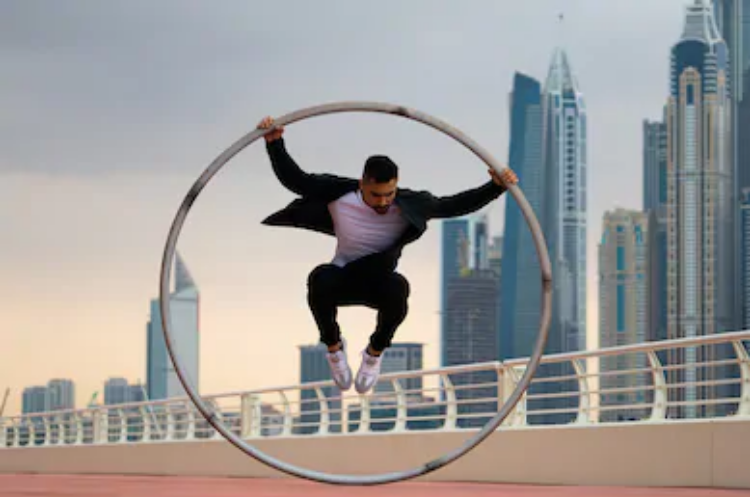
\includegraphics[width=210]{images_autres/suspension.png}
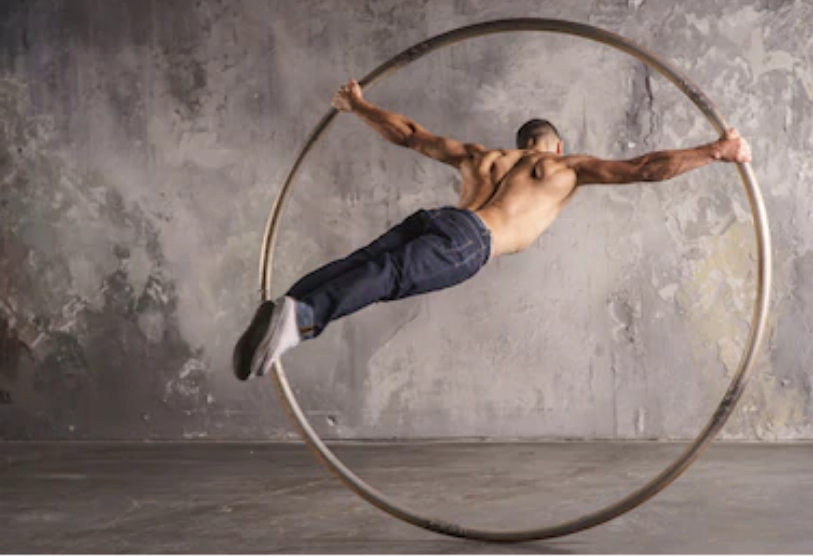
\includegraphics[width=200]{images_autres/superman.png}
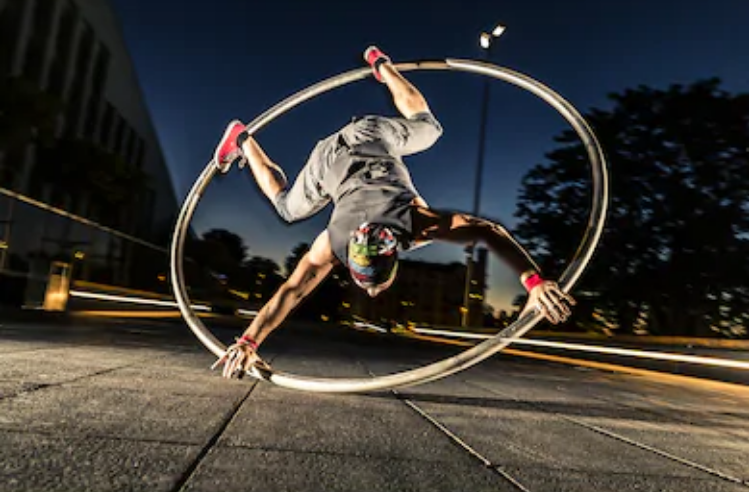
\includegraphics[width=210]{images_autres/piece.png}
\caption{Quelques figures de roue Cyr  \cite{shutterstock}. De gauche à droite: valse avec lâcher de pied, corner, saut de main, suspension, superman, pièce.}
\label{fig:figures}
\end{figure}

\clearpage

%%
%lt% anément eELEMENTt chent la roue simuS DE LA PROBLEMATIQUE
%%
\section{Problématique}  % environ 3 pages
La création d'une roue Cyr en matériaux composites enrichira la discipline de nouvelles figures et possibilités scéniques grâce à ses propriétés différentes de celles des roues Cyr classiques en métal. Ce projet se trouve au carrefour de la science, de la technique acrobatique et de l'art. Ceci nécessite de réunir des expertises issues de ces différents domaines, couplés à des moyens de fabrication adéquats. La problématique peut se découper selon les trois étapes clés du projet.

\subsection{Conception}
Il s'agit de déterminer quels paramètres parmi les propriétés mécaniques du matériau et la géométrie de la roue Cyr influencent les mouvements de cette dernière, puis de caractériser cette influence quantitativement. \\ 
A cet effet des modèles théoriques de deux mouvements caractéristiques ont été développés:
\begin{itemize}
    \item Le saut, la possibilité d’intégrer des sauts aux figures de roue Cyr déjà existante étant une des lignes directrices du projet. La roue est compressée par l'exercice d'une force verticale dont l’axe coïncide avec son diamètre, puis relâchée. Une part de l’énergie élastique stockée est convertie en saut. 
    \item Le mouvement correspondant à celui d’une pièce de monnaie qui roule sur sa tranche en décrivant des cercles, puis entre en phase terminale avant de tomber à plat sur le sol.
\end{itemize}

En se basant sur chacun des modèles théoriques correspondants, l’objectif est de déterminer séparément les paramètres géométriques et mécaniques qui :
\begin{itemize}
    \item  permettent à l’utilisateur de sauter le plus haut possible avec la roue.
    \item permettent d’optimiser le mouvement similaire à celui de la pièce de monnaie décrit ci-dessus en termes de stabilité dynamique.
    \item conduisent au meilleur compromis entre les deux réponses aux questions précédentes.
\end{itemize}


Parallèlement, il est nécessaire d’étudier les contraintes et déformations dans la roue afin d'anticiper les potentielles situations d'écoulement et de flambement et de les prendre en compte dans l'étape de conception.

\subsection{Fabrication}
Il s’agit de compléter l’étude théorique issue de la phase de conception par une utilisation adaptée de l’impression 3D. En utilisant les technologies existantes et disponibles pour le projet, comment imprimer un tore d’un diamètre avoisinant les deux mètres ? Comment assurer des propriétés conformes à celles déterminées par les modèles théoriques établis au préalable ? 

\begin{figure}[htb]
\centering
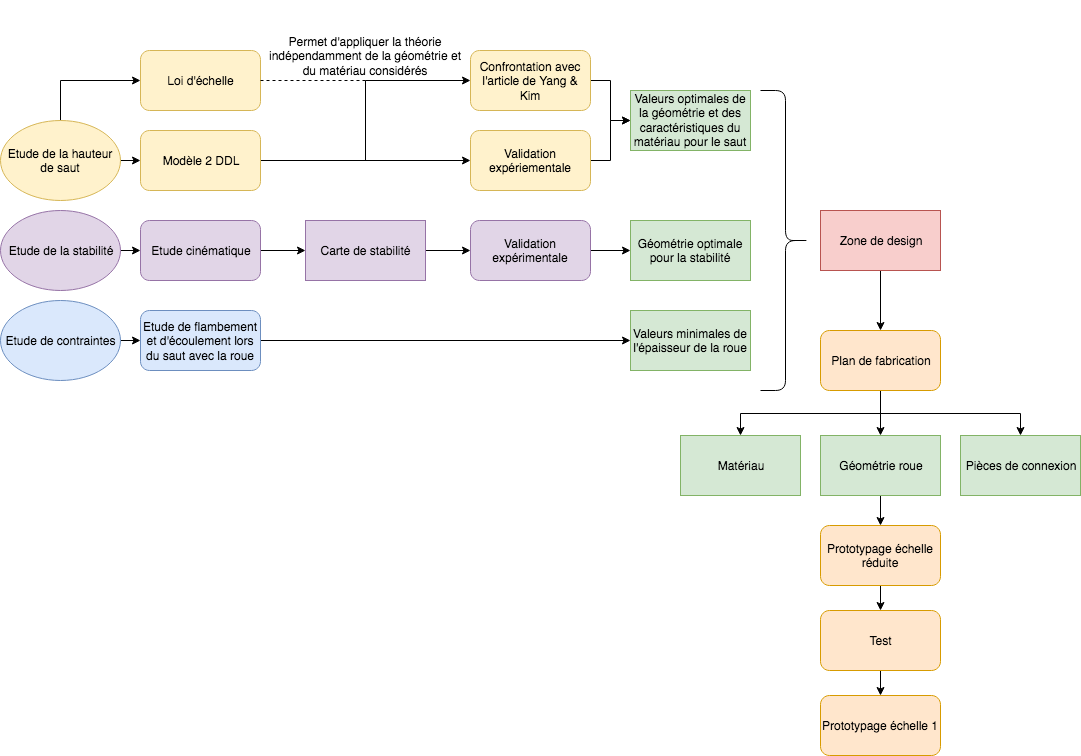
\includegraphics[width=7in]{images_autres/flowchart.png}
\caption{Flowchart résumant les étapes de conception et de fabrication de la roue.}
\label{fig:flowchart}
\end{figure}

\subsection{Tests}
Malgré la popularité du sujet au sein de la communauté circassienne, la roue en matériaux composites ne figure pas dans l'offre des fabricants d’équipement de cirque. Cela s'explique en partie par la difficulté à estimer concrètement ce qu’apporterait une telle roue Cyr et donc si les adeptes de la discipline seraient prêts à l'acquérir pour un prix supérieur à ceux des roues métalliques. Leur fabrication nécessite un investissement qui ne peut être engagé sans avoir de certitude sur sa rentabilité. Avec le prototype obtenu à l'issue de l'étape de fabrication, un phase de recherche artistique sera menée en collaboration avec des artistes de cirque. Les nouvelles possibilités introduites par une roue Cyr composite seront ainsi mises en évidence, aussi bien en termes d'acrobatie que de jeu de scène. Les fabricants seront ainsi en mesure d'évaluer si une véritable demande peut exister.\\
En outre, plusieurs artistes de roue Cyr ont déjà tenté d'approcher ces nouvelles possibilités, avec des roues Cyr fabriquées de manière artisanale dans des matériaux plus légers ou plus flexibles que les métaux (par exemple une roue Cyr en osier a été fabriquée par des élèves au Centre National des Arts du Cirque (CNAC) en France)
cependant ces projets d'expérimentation n'ont pu être menés à terme, les roues se retrouvant rapidement endommagées et hors service. Fournir un prototype fonctionnel et solide permettra à ces artistes de continuer d'approfondir leur recherche avec une sécurité accrue.

% On veut éviter que la figure et le tableau soient placés au-delà de la section courante.
\FloatBarrier


%%
%% OBJECTIFS DE RECHERCHE / RESEARCH OBJECTIVES
%%
\section{Objectifs de recherche}  % 0.5 page
\subsection{Objectif global}
L'objectif global de ce projet de recherche est de parvenir à la conception d’un prototype de roue Cyr optimisée grâce aux matériaux composites et à l'impression 3D, puis de tester avec des artistes les nouvelles possibilités offertes par cet agrès.

\subsection{Objectifs spécifiques}
Les objectifs spécifiques du projet sont les suivants:
\begin{itemize}
    \item Caractériser expérimentalement et théoriquement l’influence des propriétés mécaniques et de la géométrie sur le comportement dynamique de la roue Cyr
    \item Définir un matériau composite haute performance optimisé pour la roue Cyr
    \item Définir et mettre en oeuvre un procédé d'impression 3D adapté à nos problématiques
    \item Imprimer un prototype à partir du matériau choisi
    \item Conclure le projet par des sessions de recherche artistique autour du nouvel agrès
\end{itemize}


%%
%% PLAN DU MEMOIRE / THESIS OUTLINE
%%
\section{Plan du mémoire}  % 0.5 page
Ce mémoire s'organise en 5 chapitres. Le deuxième chapitre est constitué d'une revue de littérature centrée sur la roue Cyr, recensant les publications traitant de systèmes s'en rapprochant par leurs formes et leurs mouvements. Le chapitre trois expose une modélisation du saut d'une roue Cyr et sa validation expérimentale. Le chapitre quatre étudie la stabilité dynamique du mouvement de rotation d'une roue Cyr. Le chapitre cinq traite de la fabrication et du procédé d'impression 3D mis en oeuvre.       % Introduction au sujet de recherche.
\Chapter{REVUE DE LITTÉRATURE}\label{sec:RevLitt}

\section{Le disque d'Euler}
\subsection{Définition générale et lien avec la roue Cyr}
Le disque d'Euler est un disque plein semblable à une grosse pièce de monnaie. Son mouvement peut être découpé en deux phases:
\begin{itemize}
\item Phase 1, ou phase initiale: Le disque, incliné, roule sur sa tranche en suivant une trajectoire circulaire.
\item Phase 2, ou phase terminale: le disque se met à tourner de telle manière que le point de contact avec le sol se déplace de plus en plus lentement le long de son contour, un mouvement d'oscillation apparaît, accompagné d'un son vibratoire \cite{ringing}, et atteint sa fréquence maximale avant que le disque tombe à plat sur le sol.
\end{itemize}

C'est de la phase terminale, que le disque d'Euler tient sa popularité. Son côté spectaculaire en a fait un jouet éducatif, tandis que son comportement chaotique attise les curiosités scientifiques. Il a été déterminé que le comportement du disque au terme de cette phase était du à la viscosité de l'air.\\

\begin{figure}[h]
\centering
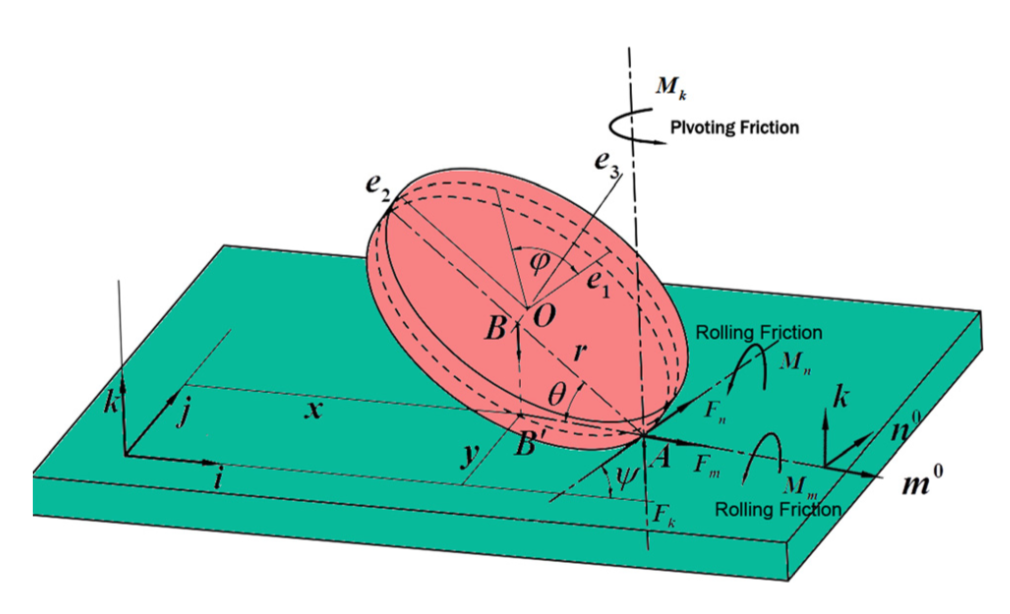
\includegraphics[width=200]{images_autres/diskma.png}
\caption{Modélisation du disque d'Euler en mouvement \cite{ma_dynamics_2016}.}
\label{fig:figures}
\end{figure}

La roue roule sur sa tranche en décrivant des cercles de plus en plus petits, avant d'entrer en phase terminale. Ces deux phases correspondent respectivement aux deux figures fondamentales de roue Cyr que sont la roue et la pièce, présentées à l'introduction. Il s'agit également de l'un des mouvements qu'on souhaite modéliser afin d'identifier les paramètres mécaniques et géométriques déterminants pour la stabilité dynamique et de caractériser leur influence. 

\subsection{Modèle mathématique et intégration numérique}
Campos et al \cite{campos} et Kessler et O'Reily \cite{ringing} développent des modèles mathématiques du disque d'Euler en vue d'une intégration numérique. Il caractérisent son comportement en termes de trajectoire du point de contact avec le sol, de variation d'énergie et de fréquence. 

\subsection{Étude de la stabilité en régime permanent}
Batista \cite{Batista} étudie la stabilité en régime permanent du mouvement du disque d'Euler correspondant à la phase 1. Il développe un modèle cinématique du disque et définit les conditions d'existence d'une position d'équilibre dynamique en fonction du signe de $\Omega_0^2$, la vitesse à laquelle le disque décrit des cercles en roulant. Ce signe dépend de l'angle d'inclinaison du disque, $\theta_0$ et du rayon des cercles décrits, $r$. Chaque couple $(\theta_0,r)$ permet de déterminer si l'équilibre dynamique est possible ou non. Avec un raisonnement similaire, Batista détermine si, en cas de stabilité, le système reste stable ou non lorsqu'on ajoute une petite perturbation. Le résultat final est une carte de stabilité d'abscisse $\theta_0$ et d'ordonnée $r_c$, où la couleur de chaque point correspond à un des trois cas: stable, indéfini (l'équilibre dynamique ne peut pas exister), ou instable en cas de perturbation.

\begin{figure}[h]
\centering
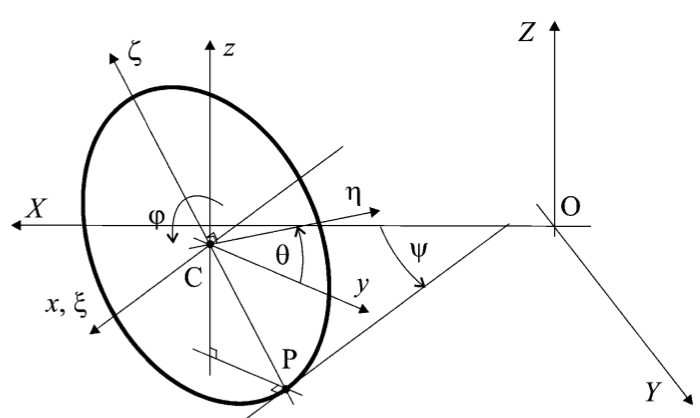
\includegraphics[width=200]{batista/ref1.png}
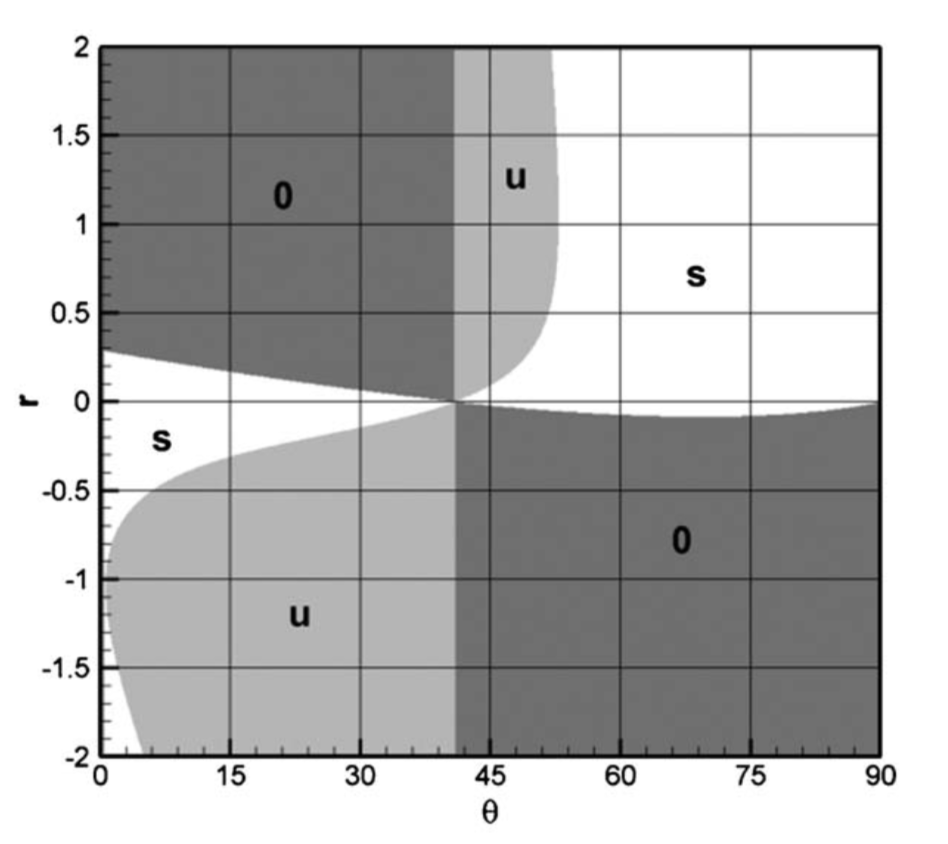
\includegraphics[width=210]{images_autres/cartebat.png}
\caption{Modèle du disque d'Euler étudié par Batista \cite{Batista}. La carte de stabilité indique si pour chaque couple $(\theta, r)$, le mouvement est stable (s), instable en cas de perturbation (u) ou si l'équilibre dynamique ne peut pas exister (0). $\theta$ décrit l'inclinaison de la roue et $r$ correspond au rayon des cercles décrits par le disque lorsqu'il roule sur sa tranche.}
\label{fig:figures}
\end{figure}

\section{Elasticité et saut d'une roue Cyr}
\subsection{Elasticité}
Afin d’étudier le stockage d’énergie élastique dans la roue lorsqu’elle est comprimée par une force verticale exercée selon son diamètre, nous avons besoin de calculer la flèche imposée par la force en question. Roark \cite{roark} développe des formules pour différents cas de chargement d’un anneau élastique, permettant entre autres de calculer les variations de diamètre horizontal et vertical en fonction des forces auxquelles l’anneau est soumis. \\
Il développe également toutes les formules nécessaires au calcul des contraintes dans la roue pour diverses géométries de section.

\subsection{Saut}
 Yang et Kim \cite{yangkim} étudient le comportement d'anneaux de diamètres millimétriques, faits de polyimides ou d'acier et de sections variables, comprimés puis relâchés. Leur saut est capturé par une caméra haute vitesse. Les résultats sont traités sous forme d'études adimensionnelles centrées sur l'énergie et la hauteur maximale de saut, $H_{max}$, puis confrontés à un modèle théorique développé à partir d'un bilan d'énergie. 
 
 \begin{figure}[h]
\centering
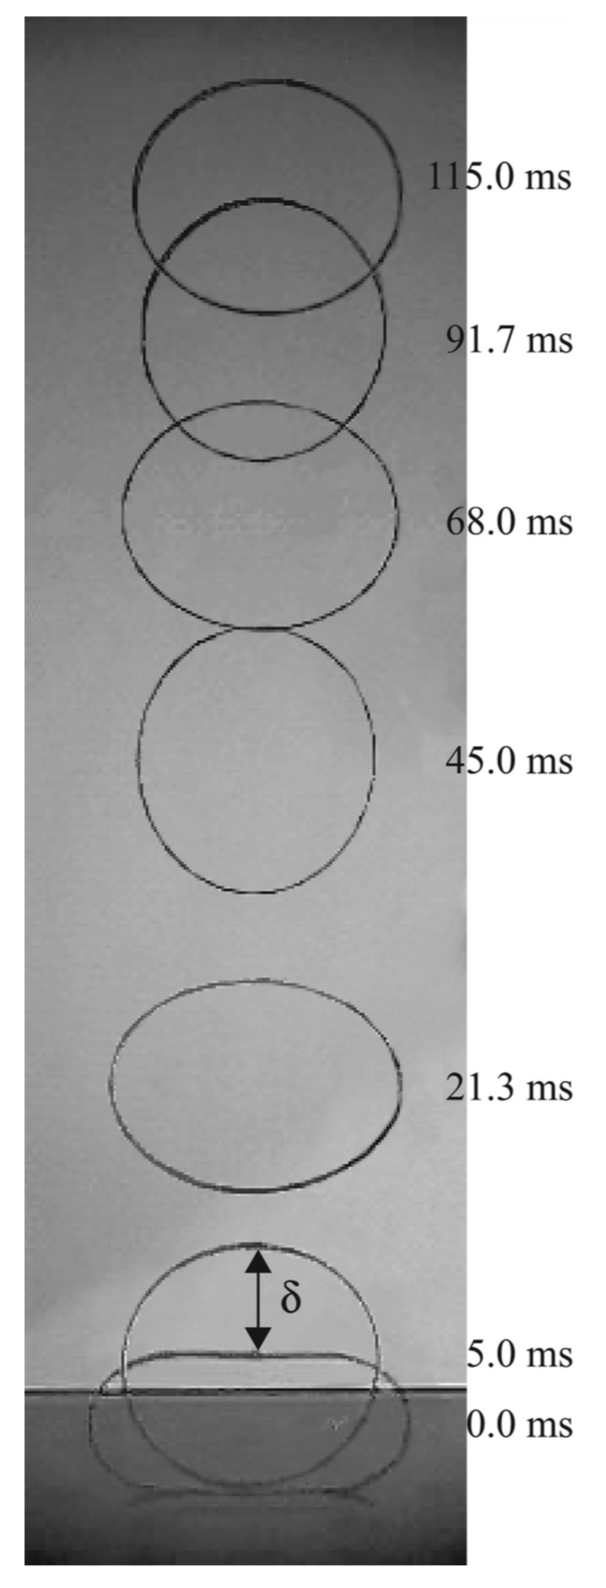
\includegraphics[width=80]{images_autres/yksaut.png}
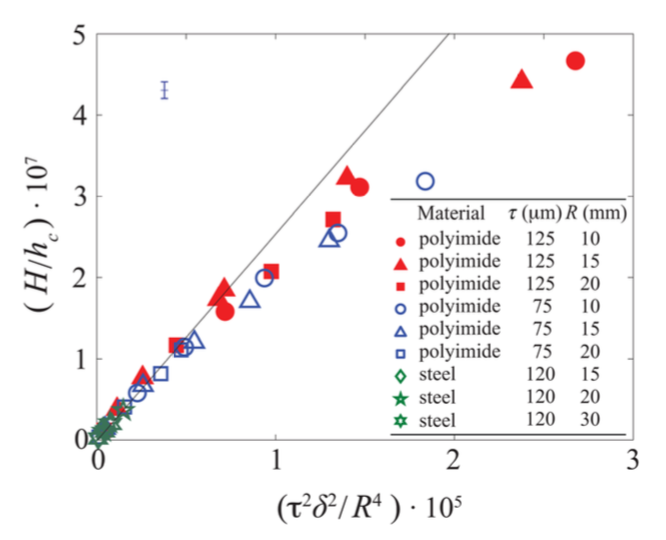
\includegraphics[width=260]{images_autres/ykres.png}
\caption{Saut d'un anneau élastique enregistré par vidéo lors d'une expérience avec un anneau en polyimide de rayon $R=16mm$, d'épaisseur $\tau=125\mu m$ et une déformation initiale de $\delta=14mm$. La figure de droite présente les résultats obtenus pour différents anneaux, sous forme de grandeurs adimensionnelles. $h_c=E/\rho g$ où $E$ est le module d'Young du matériau considéré et $\rho$ sa masse volumique \cite{yangkim}.}
\label{fig:figures}
\end{figure}  % Revue de littérature.
\Chapter{ETUDE DU SAUT D'UNE ROUE CYR}\label{sec:Theme1}
\begin{table}[htbp]
  \centering
  \caption{Constantes et variables de la modélisation du saut d'une roue Cyr}
  \begin{tabular}{|c|l|}
    \hline \rowcolor[gray]{0.8}\color{black}
    Symbole         & Description\\
    $A$           & Aire de la section\\
   
    $E$           & Module d'Young du matériau\\
    $E_{p,g}$          & Energie potentielle gravitationnelle\\
    $E_{tot}$          & Energie mécanique totale\\
    $F$             & Force de compression appliquée à la roue\\
    $g$     & Accélération gravitationnelle\\
    $H_{max}$          & Hauteur de saut maximale\\
    $I$           & Moment quadratique de la section\\
    $k$             & raideur équivalente de la roue\\
    $m_r$          & Masse de la roue\\
    
    $R$       & Rayon médian de la roue\\
    $r_1$ & Rayon interne de section pour une section circulaire\\
    $r_2$             & rayon externe de section pour une section circulaire\\
    $\rho$           & Masse volumique du matériau\\ \hline
  \end{tabular}
  \label{tab:Definitions}
\end{table}


\section{Etude théorique}
\subsection{Description du mouvement}
La roue Cyr est comprimée par une force verticale $F$ exercée selon l'axe de son diamètre puis relâchée. Une partie de l'énergie de déformation élastique est transformée en saut. On notera $H_{max}$ la hauteur correspondant à l'énergie potentielle par laquelle s'élève le centre de gravité de la roue depuis sa position au repos à sa hauteur maximale.


\subsubsection{Hypothèses}
\begin{itemize}
    \item On considère que le support contre lequel la roue est comprimée est parfaitement rigide.
    \item On néglige la force de traînée de l'air.
    \item La répartition des masses est idéalisée
\end{itemize}

\subsubsection{Modèle deux degrés de liberté}
On modélise la roue Cyr par deux masses ponctuelles égales $m_r/2$ reliées par un ressort de rigidité $k$ et de longueur à vide $2R$, où $R$ correspond au rayon médian de la roue. \\
La rigidité équivalente de la roue est donnée par \cite{yangkim}:
\begin{equation}
    k=\frac{4\pi EI}{(\pi^2 -8)R^3},
    \label{eq:0}
\end{equation}

où $E$ est le module d'Young et $I$ est le moment moment quadratique de la section de la roue.

\\
 Les positions des masses sont reperées par les ordonnées $y_1(t)$ et $y_2(t)$.

\begin{figure}[htb]
\centering

%% Creator: Inkscape inkscape 0.92.2, www.inkscape.org
%% PDF/EPS/PS + LaTeX output extension by Johan Engelen, 2010
%% Accompanies image file 'repos2.eps' (pdf, eps, ps)
%%
%% To include the image in your LaTeX document, write
%%   \input{<filename>.pdf_tex}
%%  instead of
%%   \includegraphics{<filename>.pdf}
%% To scale the image, write
%%   \def\svgwidth{<desired width>}
%%   \input{<filename>.pdf_tex}
%%  instead of
%%   \includegraphics[width=<desired width>]{<filename>.pdf}
%%
%% Images with a different path to the parent latex file can
%% be accessed with the `import' package (which may need to be
%% installed) using
%%   \usepackage{import}
%% in the preamble, and then including the image with
%%   \import{<path to file>}{<filename>.pdf_tex}
%% Alternatively, one can specify
%%   \graphicspath{{<path to file>/}}
%% 
%% For more information, please see info/svg-inkscape on CTAN:
%%   http://tug.ctan.org/tex-archive/info/svg-inkscape
%%
\begingroup%
  \makeatletter%
  \providecommand\color[2][]{%
    \errmessage{(Inkscape) Color is used for the text in Inkscape, but the package 'color.sty' is not loaded}%
    \renewcommand\color[2][]{}%
  }%
  \providecommand\transparent[1]{%
    \errmessage{(Inkscape) Transparency is used (non-zero) for the text in Inkscape, but the package 'transparent.sty' is not loaded}%
    \renewcommand\transparent[1]{}%
  }%
  \providecommand\rotatebox[2]{#2}%
  \ifx\svgwidth\undefined%
    \setlength{\unitlength}{337.82993867bp}%
    \ifx\svgscale\undefined%
      \relax%
    \else%
      \setlength{\unitlength}{\unitlength * \real{\svgscale}}%
    \fi%
  \else%
    \setlength{\unitlength}{\svgwidth}%
  \fi%
  \global\let\svgwidth\undefined%
  \global\let\svgscale\undefined%
  \makeatother%
  \begin{picture}(1,0.62816437)%
    \put(0,0){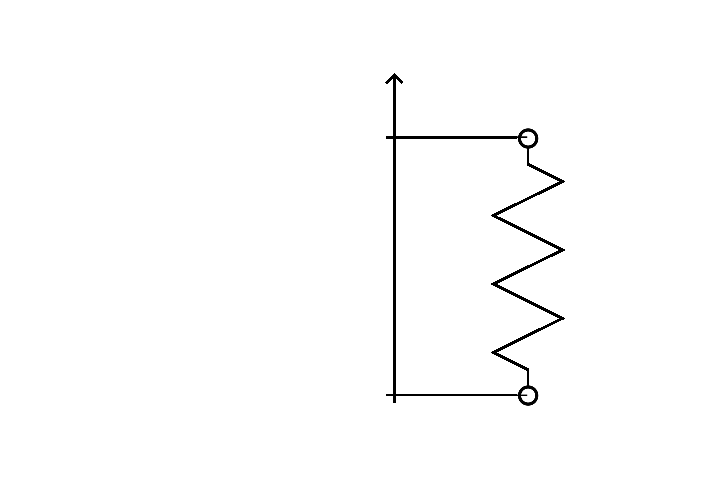
\includegraphics[width=\unitlength]{images_2ddl/repos2.eps}}%
    \put(0.53610169,0.57938811){\color[rgb]{0,0,0}\makebox(0,0)[lb]{\smash{$y$}}}%
    \put(0.29,0.46){\color[rgb]{0,0,0}\makebox(0,0)[lb]{\smash{$y_1=2R-\dfrac{m_r g}{2k}$}}}%
    \put(0.42,0.09){\color[rgb]{0,0,0}\makebox(0,0)[lb]{\smash{$y_2=0$}}}%
    \put(0.62490379,0.2696811){\color[rgb]{0,0,0}\makebox(0,0)[lb]{\smash{$k$}}}%
    \put(0.7581069,0.49168631){\color[rgb]{0,0,0}\makebox(0,0)[lb]{\smash{$\dfrac{m_r}{2}$}}}%
    \put(0.78030738,0.0698765){\color[rgb]{0,0,0}\makebox(0,0)[lb]{\smash{$\dfrac{m_r}{2}$}}}%
  \end{picture}%
\endgroup%

\caption{Système au repos. Le ressort de longueur à vide $2R$ et de raideur $k$ est écrasé par le poids de la masse supérieure.}
\label{fig:repos}
\end{figure}

\subsection{Limite en comportement linéaire}

A partir d'une certaine flèche $\delta$ imposée par une force de compression $F$, l'anneau ne se comporte plus de manière linéaire et la relation $F=k\delta$, où $k$ est la constante définie dans l'équation \ref{eq:0}, n'est plus valable. 
La valeur limite de $\delta$ au delà de laquelle on sort du domaine de comportement linéaire, est définie avec une étude éléments finis prenant en compte les non linéarités d'ordre géométrique, que l'on compare avec le modèle théorique linéaire (figure \ref{fig:lin1}). Dans cette étude, la roue est modélisée avec des éléments poutres, le déplacement $\delta$ est imposé comme paramètre d'entrée et la force $F$, relevée comme donnée de sortie, pour des raisons de convergence.

On considère qu'on sort de la zone de comportement linéaire lorsque la valeur absolue de l'erreur relative entre les deux modèles, $\epsilon=\frac{F_{éléments finis}-F_{théorique}}{F_{théorique}}$ dépasse 10\%. La limite du domaine de comportement linéaire correspond donc à $\frac{delta}{R}<0.1$

\begin{figure}[h]
\centering
%% Creator: Inkscape inkscape 0.92.2, www.inkscape.org
%% PDF/EPS/PS + LaTeX output extension by Johan Engelen, 2010
%% Accompanies image file 'lineaire.eps' (pdf, eps, ps)
%%
%% To include the image in your LaTeX document, write
%%   \input{<filename>.pdf_tex}
%%  instead of
%%   \includegraphics{<filename>.pdf}
%% To scale the image, write
%%   \def\svgwidth{<desired width>}
%%   \input{<filename>.pdf_tex}
%%  instead of
%%   \includegraphics[width=<desired width>]{<filename>.pdf}
%%
%% Images with a different path to the parent latex file can
%% be accessed with the `import' package (which may need to be
%% installed) using
%%   \usepackage{import}
%% in the preamble, and then including the image with
%%   \import{<path to file>}{<filename>.pdf_tex}
%% Alternatively, one can specify
%%   \graphicspath{{<path to file>/}}
%% 
%% For more information, please see info/svg-inkscape on CTAN:
%%   http://tug.ctan.org/tex-archive/info/svg-inkscape
%%
\begingroup%
  \makeatletter%
  \providecommand\color[2][]{%
    \errmessage{(Inkscape) Color is used for the text in Inkscape, but the package 'color.sty' is not loaded}%
    \renewcommand\color[2][]{}%
  }%
  \providecommand\transparent[1]{%
    \errmessage{(Inkscape) Transparency is used (non-zero) for the text in Inkscape, but the package 'transparent.sty' is not loaded}%
    \renewcommand\transparent[1]{}%
  }%
  \providecommand\rotatebox[2]{#2}%
  \ifx\svgwidth\undefined%
    \setlength{\unitlength}{344.79999138bp}%
    \ifx\svgscale\undefined%
      \relax%
    \else%
      \setlength{\unitlength}{\unitlength * \real{\svgscale}}%
    \fi%
  \else%
    \setlength{\unitlength}{\svgwidth}%
  \fi%
  \global\let\svgwidth\undefined%
  \global\let\svgscale\undefined%
  \makeatother%
  \begin{picture}(1,0.83526682)%
    \put(0,0){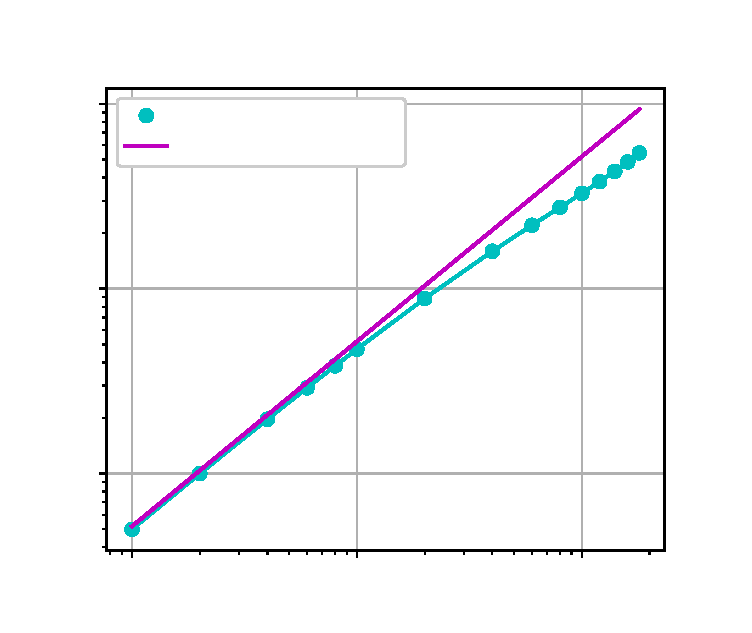
\includegraphics[width=\unitlength]{images_2ddl/lineaire.eps}}%
    \put(0.1257964,0.0485348){\color[rgb]{0,0,0}\makebox(0,0)[lb]{\smash{10}}}%
    \put(0.16297825,0.05963727){\color[rgb]{0,0,0}\makebox(0,0)[lb]{\smash{-2}}}%
    \put(0.43892111,0.04878857){\color[rgb]{0,0,0}\makebox(0,0)[lb]{\smash{10}}}%
    \put(0.47610296,0.05989104){\color[rgb]{0,0,0}\makebox(0,0)[lb]{\smash{-1}}}%
    \put(0.76074536,0.0485348){\color[rgb]{0,0,0}\makebox(0,0)[lb]{\smash{10}}}%
    \put(0.7979272,0.05963727){\color[rgb]{0,0,0}\makebox(0,0)[lb]{\smash{0}}}%
    \put(0.45736079,0.00605084){\color[rgb]{0,0,0}\makebox(0,0)[lb]{\smash{$\delta/R$ }}}%
    \put(0.05278422,0.18847651){\color[rgb]{0,0,0}\makebox(0,0)[lb]{\smash{10}}}%
    \put(0.08996607,0.19957897){\color[rgb]{0,0,0}\makebox(0,0)[lb]{\smash{2}}}%
    \put(0.05278422,0.44581787){\color[rgb]{0,0,0}\makebox(0,0)[lb]{\smash{10}}}%
    \put(0.08996607,0.45692033){\color[rgb]{0,0,0}\makebox(0,0)[lb]{\smash{3}}}%
    \put(0.05278422,0.70196636){\color[rgb]{0,0,0}\makebox(0,0)[lb]{\smash{10}}}%
    \put(0.08996607,0.71306882){\color[rgb]{0,0,0}\makebox(0,0)[lb]{\smash{4}}}%
    \put(0.03515632,0.373692){\color[rgb]{0,0,0}\rotatebox{90}{\makebox(0,0)[lb]{\smash{$F (N)$ }}}}%
    \put(0.23259861,0.68690835){\color[rgb]{0,0,0}\makebox(0,0)[lb]{\smash{étude éléments finis}}}%
    \put(0.23259861,0.64435615){\color[rgb]{0,0,0}\makebox(0,0)[lb]{\smash{théorie}}}%
  \end{picture}%
\endgroup%

\caption{Comparaison entre une étude éléments finis d'une roue en éléments poutres, dans laquelle on prend en compte les non linéarités géométriques, et le modèle théorique linéaire où la force appliquée et le déplacement sont liés par la constante $k$ selon la relation $F=k \delta$.}
\label{fig:lin1}
\end{figure}

La dérivation de la courbe de $F=f(\delta)$ obtenue par analyse éléments finis donne l'évolution de la raideur $k$ en fonction de $\delta/R$ (figure \ref{fig:lin2}).\\
Dans le domaine linéaire, on prendra comme valeur de $k$ la valeur moyenne des points situés dans la zone $\delta/R<0.1$

\begin{figure}[h]
\centering
%% Creator: Inkscape inkscape 0.92.2, www.inkscape.org
%% PDF/EPS/PS + LaTeX output extension by Johan Engelen, 2010
%% Accompanies image file 'lineaire2.eps' (pdf, eps, ps)
%%
%% To include the image in your LaTeX document, write
%%   \input{<filename>.pdf_tex}
%%  instead of
%%   \includegraphics{<filename>.pdf}
%% To scale the image, write
%%   \def\svgwidth{<desired width>}
%%   \input{<filename>.pdf_tex}
%%  instead of
%%   \includegraphics[width=<desired width>]{<filename>.pdf}
%%
%% Images with a different path to the parent latex file can
%% be accessed with the `import' package (which may need to be
%% installed) using
%%   \usepackage{import}
%% in the preamble, and then including the image with
%%   \import{<path to file>}{<filename>.pdf_tex}
%% Alternatively, one can specify
%%   \graphicspath{{<path to file>/}}
%% 
%% For more information, please see info/svg-inkscape on CTAN:
%%   http://tug.ctan.org/tex-archive/info/svg-inkscape
%%
\begingroup%
  \makeatletter%
  \providecommand\color[2][]{%
    \errmessage{(Inkscape) Color is used for the text in Inkscape, but the package 'color.sty' is not loaded}%
    \renewcommand\color[2][]{}%
  }%
  \providecommand\transparent[1]{%
    \errmessage{(Inkscape) Transparency is used (non-zero) for the text in Inkscape, but the package 'transparent.sty' is not loaded}%
    \renewcommand\transparent[1]{}%
  }%
  \providecommand\rotatebox[2]{#2}%
  \ifx\svgwidth\undefined%
    \setlength{\unitlength}{395.9999901bp}%
    \ifx\svgscale\undefined%
      \relax%
    \else%
      \setlength{\unitlength}{\unitlength * \real{\svgscale}}%
    \fi%
  \else%
    \setlength{\unitlength}{\svgwidth}%
  \fi%
  \global\let\svgwidth\undefined%
  \global\let\svgscale\undefined%
  \makeatother%
  \begin{picture}(1,0.833939)%
    \put(0,0){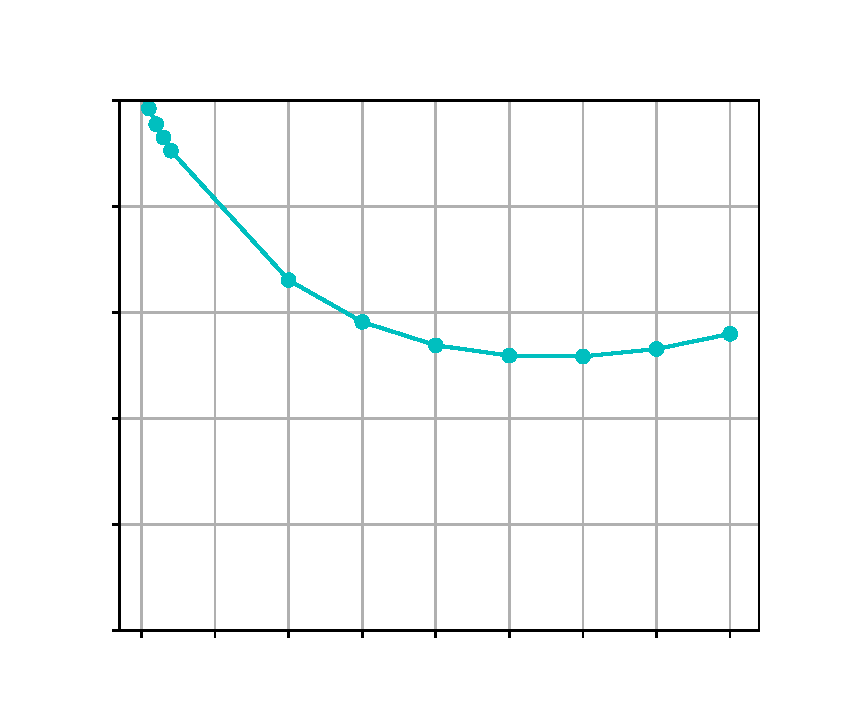
\includegraphics[width=\unitlength]{images_2ddl/lineaire2.eps}}%
    \put(0.13122525,0.05494683){\color[rgb]{0,0,0}\makebox(0,0)[lb]{\smash{0.0}}}%
    \put(0.22040808,0.05494683){\color[rgb]{0,0,0}\makebox(0,0)[lb]{\smash{0.2}}}%
    \put(0.30959091,0.05494683){\color[rgb]{0,0,0}\makebox(0,0)[lb]{\smash{0.4}}}%
    \put(0.39877273,0.05494683){\color[rgb]{0,0,0}\makebox(0,0)[lb]{\smash{0.6}}}%
    \put(0.48795707,0.05494683){\color[rgb]{0,0,0}\makebox(0,0)[lb]{\smash{0.8}}}%
    \put(0.57714141,0.05494683){\color[rgb]{0,0,0}\makebox(0,0)[lb]{\smash{1.0}}}%
    \put(0.66632323,0.05494683){\color[rgb]{0,0,0}\makebox(0,0)[lb]{\smash{1.2}}}%
    \put(0.75550505,0.05494683){\color[rgb]{0,0,0}\makebox(0,0)[lb]{\smash{1.4}}}%
    \put(0.84468939,0.05494683){\color[rgb]{0,0,0}\makebox(0,0)[lb]{\smash{1.6}}}%
    \put(0.09126414,0.08221173){\color[rgb]{0,0,0}\makebox(0,0)[lb]{\smash{0}}}%
    \put(0.04308712,0.21073142){\color[rgb]{0,0,0}\makebox(0,0)[lb]{\smash{1000}}}%
    \put(0.04308712,0.33925213){\color[rgb]{0,0,0}\makebox(0,0)[lb]{\smash{2000}}}%
    \put(0.04308712,0.46777233){\color[rgb]{0,0,0}\makebox(0,0)[lb]{\smash{3000}}}%
    \put(0.04308712,0.59629254){\color[rgb]{0,0,0}\makebox(0,0)[lb]{\smash{4000}}}%
    \put(0.04308712,0.72481274){\color[rgb]{0,0,0}\makebox(0,0)[lb]{\smash{5000}}}%
    \put(0.48795707,0.01){\color[rgb]{0,0,0}\makebox(0,0)[lb]{\smash{$\delta/R$ }}}%
    \put(0.02773838,0.36184557){\color[rgb]{0,0,0}\rotatebox{90}{\makebox(0,0)[lb]{\smash{$k$ $ (N \cdot m^{-1})$ }}}}%
  \end{picture}%
\endgroup%

\caption{Évolution du coefficient de raideur $k$ en fonction du ratio $\delta/R$. Cette courbe est obtenue par la dérivation des points de l'analyse éléments finis (figure \ref{fig:lin1}), en utilisant la méthode des différences finies centrées.}
\label{fig:lin2}
\end{figure}

\subsection{Mise en équations}

Les variables temporelles suivantes décrivent le mouvement du système comprimé puis relâché  (figure \ref{fig:saut}):

\begin{itemize}
    \item[$\bullet$] $t=-t_0$ : on relâche le ressort
    \item[$\bullet$] $t=0$ : la masse inférieure quitte le sol
    \item[$\bullet$] $t=t_f$ : le centre de gravité du système atteint sa hauteur maximale
\end{itemize}



\begin{figure}[h]

\def\svgwidth{400}
%% Creator: Inkscape inkscape 0.92.2, www.inkscape.org
%% PDF/EPS/PS + LaTeX output extension by Johan Engelen, 2010
%% Accompanies image file 'saut1.eps' (pdf, eps, ps)
%%
%% To include the image in your LaTeX document, write
%%   \input{<filename>.pdf_tex}
%%  instead of
%%   \includegraphics{<filename>.pdf}
%% To scale the image, write
%%   \def\svgwidth{<desired width>}
%%   \input{<filename>.pdf_tex}
%%  instead of
%%   \includegraphics[width=<desired width>]{<filename>.pdf}
%%
%% Images with a different path to the parent latex file can
%% be accessed with the `import' package (which may need to be
%% installed) using
%%   \usepackage{import}
%% in the preamble, and then including the image with
%%   \import{<path to file>}{<filename>.pdf_tex}
%% Alternatively, one can specify
%%   \graphicspath{{<path to file>/}}
%% 
%% For more information, please see info/svg-inkscape on CTAN:
%%   http://tug.ctan.org/tex-archive/info/svg-inkscape
%%
\begingroup%
  \makeatletter%
  \providecommand\color[2][]{%
    \errmessage{(Inkscape) Color is used for the text in Inkscape, but the package 'color.sty' is not loaded}%
    \renewcommand\color[2][]{}%
  }%
  \providecommand\transparent[1]{%
    \errmessage{(Inkscape) Transparency is used (non-zero) for the text in Inkscape, but the package 'transparent.sty' is not loaded}%
    \renewcommand\transparent[1]{}%
  }%
  \providecommand\rotatebox[2]{#2}%
  \ifx\svgwidth\undefined%
    \setlength{\unitlength}{458.93788937bp}%
    \ifx\svgscale\undefined%
      \relax%
    \else%
      \setlength{\unitlength}{\unitlength * \real{\svgscale}}%
    \fi%
  \else%
    \setlength{\unitlength}{\svgwidth}%
  \fi%
  \global\let\svgwidth\undefined%
  \global\let\svgscale\undefined%
  \makeatother%
  \begin{picture}(1,0.55996795)%
    \put(0,0){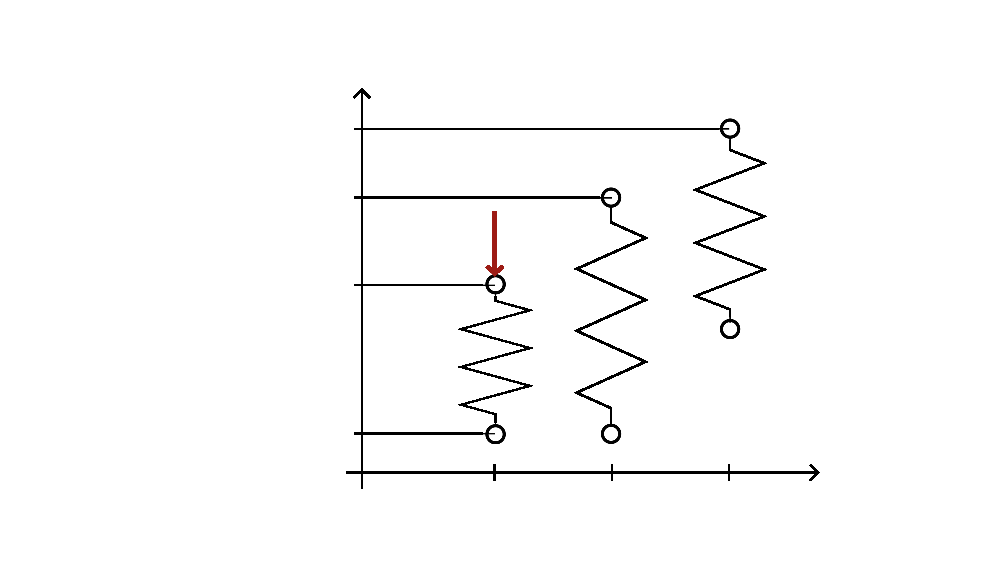
\includegraphics[width=\unitlength]{images_2ddl/saut1.eps}}%
    \put(0.35332121,0.50424636){\color[rgb]{0,0,0}\makebox(0,0)[lb]{\smash{$y$}}}%
    \put(0.85079889,0.07843695){\color[rgb]{0,0,0}\makebox(0,0)[lb]{\smash{$t$}}}%
    \put(0.44868441,0.03798154){\color[rgb]{0,0,0}\makebox(0,0)[lb]{\smash{$t<-t_0$}}}%
    \put(0.59510438,0.04003324){\color[rgb]{0,0,0}\makebox(0,0)[lb]{\smash{$t=0$}}}%
    \put(0.71660123,0.03978188){\color[rgb]{0,0,0}\makebox(0,0)[lb]{\smash{$t=t_f$}}}%
    \put(0.31206609,0.11596114){\color[rgb]{0,0,0}\makebox(0,0)[lb]{\smash{$0$}}}%
    \put(0.12576987,0.27218246){\color[rgb]{0,0,0}\makebox(0,0)[lb]{\smash{$2R-\dfrac{F}{k}-\dfrac{m_r g}{2k}$}}}%
    \put(0.19576987,0.36438468){\color[rgb]{0,0,0}\makebox(0,0)[lb]{\smash{$2R+\dfrac{m_r g}{2k}$}}}%
    \put(0.25429501,0.44056847){\color[rgb]{0,0,0}\makebox(0,0)[lb]{\smash{$y_{1,max}$}}}%
    \put(0.51238222,0.3284082){\color[rgb]{0.61568627,0.10588235,0.07843137}\makebox(0,0)[lb]{\smash{$F$}}}%
  \end{picture}%
\endgroup%


\caption{Saut du système. Pour $t<-t_0$, le système est écrasé par une force F. Il est relâché à $t=-t_0$, et la masse inférieure quitte le sol à $t=0$. Le centre de gravité du système atteint sa hauteur maximale pour $t=t_f$}
\label{fig:saut}
\end{figure}

Pour $-t_0<t<0$, la masse supérieure est soumise à deux forces verticales: son propre poids de norme $-m_r g/2$, et la force élastique de norme $-k(y_1-2R)$. Son mouvement est régi par:

\begin{equation}
    \frac{m_r}{2}\frac{d^2y_1}{dt^2}+k(y_1-2R)+\frac{m_r}{2}g=0,
  \label{eq:1}
\end{equation}

avec les condition initiales:
\begin{align}
    &y_1(-t_0)=2R-\frac{F}{k}-\frac{m_r g}{2k} \nonumber\\
    &\frac{dy_1}{dt}(-t_0)=0,
\label{eq:1i}
\end{align}

où $g$ est l'accélération gravitationnelle. \\
  
Pour $0<t<t_f$, la force que le ressort exerce sur la masse inférieure devient suffisante pour prendre le dessus sur la gravité: $m_r g/2=k(y_1-2R)$,  et le mouvement des deux masses est régi par:

\begin{align}
    \frac{m_r}{2}\frac{d^2y_1}{dt^2}+k(y_1-y_2-2R)+\frac{m_r}{2}g&=0 \nonumber\\
    \frac{m_r}{2}\frac{d^2y_2}{dt^2}+k(y_2-y_1+2R)+\frac{m_r}{2}g&=0,
  \label{eq:3}
\end{align}

avec les conditions initiales: 
\begin{align}
    y_1(0)=&2R+\frac{m_r g}{2k} & \frac{d y_1}{dt}(0)=&v_{10}\nonumber\\
    y_2(0)=&0 & \frac{d y2}{dt}(0)=&0
  \label{eq:4}
\end{align}    
    

\begin{figure}[htb]
\centering
\def\svgwidth{350}
%% Creator: Inkscape inkscape 0.92.2, www.inkscape.org
%% PDF/EPS/PS + LaTeX output extension by Johan Engelen, 2010
%% Accompanies image file 'sautp.eps' (pdf, eps, ps)
%%
%% To include the image in your LaTeX document, write
%%   \input{<filename>.pdf_tex}
%%  instead of
%%   \includegraphics{<filename>.pdf}
%% To scale the image, write
%%   \def\svgwidth{<desired width>}
%%   \input{<filename>.pdf_tex}
%%  instead of
%%   \includegraphics[width=<desired width>]{<filename>.pdf}
%%
%% Images with a different path to the parent latex file can
%% be accessed with the `import' package (which may need to be
%% installed) using
%%   \usepackage{import}
%% in the preamble, and then including the image with
%%   \import{<path to file>}{<filename>.pdf_tex}
%% Alternatively, one can specify
%%   \graphicspath{{<path to file>/}}
%% 
%% For more information, please see info/svg-inkscape on CTAN:
%%   http://tug.ctan.org/tex-archive/info/svg-inkscape
%%
\begingroup%
  \makeatletter%
  \providecommand\color[2][]{%
    \errmessage{(Inkscape) Color is used for the text in Inkscape, but the package 'color.sty' is not loaded}%
    \renewcommand\color[2][]{}%
  }%
  \providecommand\transparent[1]{%
    \errmessage{(Inkscape) Transparency is used (non-zero) for the text in Inkscape, but the package 'transparent.sty' is not loaded}%
    \renewcommand\transparent[1]{}%
  }%
  \providecommand\rotatebox[2]{#2}%
  \ifx\svgwidth\undefined%
    \setlength{\unitlength}{431.9999892bp}%
    \ifx\svgscale\undefined%
      \relax%
    \else%
      \setlength{\unitlength}{\unitlength * \real{\svgscale}}%
    \fi%
  \else%
    \setlength{\unitlength}{\svgwidth}%
  \fi%
  \global\let\svgwidth\undefined%
  \global\let\svgscale\undefined%
  \makeatother%
  \begin{picture}(1,0.83333334)%
    \put(0,0){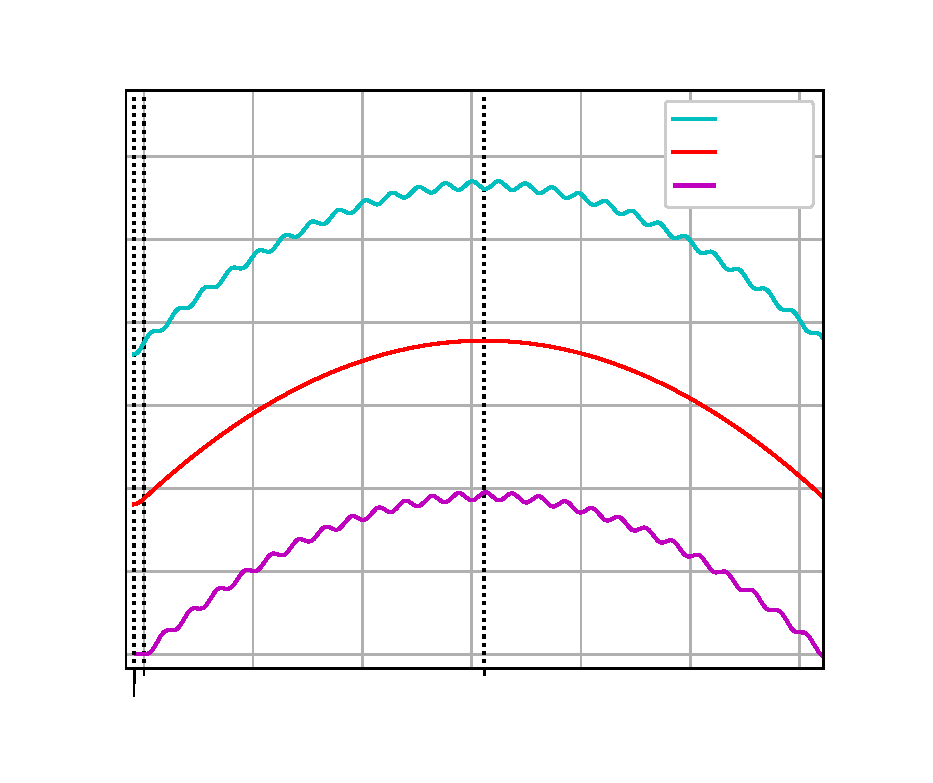
\includegraphics[width=\unitlength]{images_2ddl/sautp.eps}}%
    \put(0.79467593,0.71228239){\color[rgb]{0,0,0}\makebox(0,0)[lb]{\smash{$y_1(t)$}}}%
    \put(0.79467593,0.67524535){\color[rgb]{0,0,0}\makebox(0,0)[lb]{\smash{$y_{cdg}(t)$}}}%
    \put(0.79467593,0.63820832){\color[rgb]{0,0,0}\makebox(0,0)[lb]{\smash{$y_2(t)$}}}%
    \put(0.09341219,0.0388418){\color[rgb]{0,0,0}\makebox(0,0)[lb]{\smash{$-t_0$}}}%
    \put(0.135556003,0.06552941){\color[rgb]{0,0,0}\makebox(0,0)[lb]{\smash{$0$}}}%
    \put(0.5175824,0.06311792){\color[rgb]{0,0,0}\makebox(0,0)[lb]{\smash{$t_f$}}}%
    \put(0.05446337,0.76775099){\color[rgb]{0,0,0}\makebox(0,0)[lb]{\smash{$y (m)$}}}%
    \put(0.86146302,0.06058865){\color[rgb]{0,0,0}\makebox(0,0)[lb]{\smash{$t (s)$}}}%
  \end{picture}%
\endgroup%


\caption{Évolution temporelle des positions des masses et du centre de gravité lors du saut du système}
\label{fig:saut}
\end{figure}

Avant de résoudre le problème, on le réécrit sous forme adimensionnelle:
on définit le temps adimensionnel $\tau=t\sqrt{\dfrac{2k}{m_r}}$ et les variables positions adimensionnelles $\xi_1=y_1 \dfrac{2k}{m_r g}$ et $\xi_2=y_2 \dfrac{2k}{m_r g}$ \\

 L'équation \ref{eq:1} devient:
\begin{equation}
    \frac{d^2\xi_1}{d\tau^2}+\xi_1-\xi_0+1=0,
  \label{eq:1a}
\end{equation}
\\
pour $-\tau_0<\tau<0$,\\
avec $\xi_0=\dfrac{4Rk}{m_r g}$ et $\tau_0=t_0 \sqrt{\frac{2k}{m_r}}$ \\

et avec les conditions initiales
\begin{align}
    &\xi_1(-\tau_0)=\xi_0-\frac{2F}{m_r g}-1 \nonumber\\
    &\frac{d\xi_1}{d\tau}(-\tau_0)=0
\label{eq:1ia}
\end{align}
 

De même, l'équation \ref{eq:3} devient:
\begin{align}
    \frac{d^2\xi_1}{d\tau^2}+\xi_1-\xi_2-\xi_0+1&=0 \nonumber\\
    \frac{d^2\xi_2}{d\tau^2}+\xi_2-\xi_1+\xi_0+1&=0
  \label{eq:3a}
\end{align}

pour $0<\tau<\tau_f$,\\
avec $\tau_f=t_f \sqrt{\frac{2k}{m_r}}$ \\
et avec les conditions initiales: 
\begin{align}
    \xi_1(0)&=\xi_0+1   &  \frac{d xi_1}{d\tau}(0)&=\zeta_{10} \nonumber\\
    \xi_2(0)&=0   &  \frac{d \xi_2}{d\tau}(0)&=0
  \label{eq:4a}
\end{align} 

En résolvant \ref{eq:1a} avec les conditions initiales \ref{eq:1ia}, on obtient l'équation du mouvement \ref{eq:2} pour $-\tau_0<\tau<0$:
\begin{align}
    \xi_1&=-frac{-2F}{m_r g}(\cos{-\tau_0}\cos{\tau}+\sin{-\tau_0}\sin{\tau})+\xi_0-1 \nonumber\\
    \xi_2&=0
  \label{eq:2}
\end{align}

En résolvant \ref{eq:3a} avec les conditions initiales \ref{eq:4a}, on obtient l'équation du mouvement \ref{eq:5a} pour $0<\tau<\tau_f$:
\begin{align}
    \xi_1&=-\frac{1}{2}\tau^2+\frac{\zeta_{10}}{2}\tau+\frac{\zeta_{10}}{2\sqrt{2}}\sin{(\sqrt{2}\tau)}+\frac{1}{2}\cos{(\sqrt{2}\tau)}+\xi_0+\frac{1}{2} \nonumber\\
    \xi_2&=-\frac{1}{2}\tau^2+\frac{\zeta_{10}}{2}\tau-\frac{\zeta_{10}}{2\sqrt{2}}\sin{(\sqrt{2}\tau)}-\frac{1}{2}\cos{(\sqrt{2}\tau)}-\frac{1}{2}
  \label{eq:5a}
\end{align}

La vitesse initiale adimensionnelle de la masse supérieure s'exprime
\begin{equation}
    \zeta_{10}=\frac{d\xi_1}{d\tau}(0)=-\frac{2F}{m_r g}\sin{-\tau_0}
    \label{eq:c1}
\end{equation}


D'après les conditions initiales \ref{eq:4a} appliquées à l'équation \ref{eq:2}, on a par continuité:
\begin{equation}
    \cos{-\tau_0}=-\frac{m_r g}{F}
    \label{eq:c2}
\end{equation}

On substitue \ref{eq:c2} à l'intérieur de \ref{eq:c1}:
\begin{equation}
    \zeta_{10}=\sqrt{(\frac{2F}{m_r g})^2-4}
    \label{eq:c3}
\end{equation}

La positon adimensionnelle du centre de gravité du système s'écrit $\xi_{cdg}(\tau)=\dfrac{\xi_1(\tau)+\xi_2(\tau)}{2}$. En substituant \ref{eq:5a} dans cette expression, on obtient: 

\begin{equation}
  \xi_{cdg}(\tau)=-\frac{1}{2}\tau^2+\frac{\zeta_{10}}{2}\tau+\frac{\xi_0+1}{2}
  \label{eq:cdg}
\end{equation}

En substituant \ref{eq:c3} dans \ref{eq:cdg} on obtient:

\begin{equation}
  \xi_{cdg}(\tau)=-\frac{1}{2}\tau^2+\sqrt{(\frac{F}{m_r g})^2-1}\tau+\frac{\xi_0+1}{2}
  \label{eq:cdg2}
\end{equation}

Durant l'élévation du centre de gravité de la roue, on observe des déformations correspondant au second mode vibratoire d'un anneau (déformations planes).

Lorsqu'on arrive à $\tau=\tau_f$, la vitesse du centre de gravité s'annule. En dérivant \ref{eq:cdg2}, on trouve l'expression de $\tau_f$:

\begin{equation}
    \tau_f=\sqrt{(\frac{F}{m_r g})^2-1}
    \label{eq:tauf}
\end{equation}

On substitue ensuite \ref{eq:tauf} à l'intérieur de \ref{eq:cdg2} pour obtenir l'expression de la hauteur maximale du centre de gravité:

\begin{equation}
  \xi_{cdg,max}=\frac{1}{2}((\frac{F}{m_r g})^2-1)+\frac{\xi_0+1}{2}
  \label{eq:cdgmax}
\end{equation}

On soustrait ensuite à \ref{eq:cdgmax} sa position adimensionnelle à l'équilibre statique $\xi_{cdg,ref}=\dfrac{\xi_0-1}{2}$ pour obtenir l'expression adimensionnelle $\eta_{max}=\dfrac{2k}{m_rg}H_{max}$:


\begin{equation}
\eta_{max}=\frac{1}{2}((\frac{F}{m_r g})^2+1)
 \label{eq:hmax}
\end{equation}


Ainsi, les paramètres influençant la hauteur maximale de saut du système sont:
\begin{itemize}
    \item La force de compression $F$ à laquelle ce dernier est soumis initialement
    \item La masse du système, déterminée par sa géométrie et la masse volumique du matériau
    \item La raideur équivalente du système qui dépend de sa géométrie et du module de Young du matériau.
\end{itemize}

L'expression de $H_{max}$ permet d'étudier l'efficacité énergétique du système, c'est à dire la fraction de l'énergie totale $E_{tot}$ fournie au système sous forme de déformation élastique qui est convertie en énergie potentielle gravitationnelle $E_{p,g}$ servant au saut. \\
Avec $E_{tot}=\dfrac{F^2}{2k}$ et $E_{p,g}=m_r g H_{max}$,\\
L'efficacité énergétique s'exprime:  $\dfrac{E_{p,g}}{E_{tot}}=\dfrac{1}{2}((\dfrac{m_r g}{F})^2+1)$.

\subsection{Valeurs limites et premiers résultats}
Dans la partie qui suit, on étudie les variations de $\eta_{max}$, la hauteur maximale de saut adimensionnelle et du ratio d'efficacité énergétique.
\\ 
\\ 
Les paramètres $F$, $k$ et $m_r$ doivent rester supérieurs aux valeurs limites suivantes, en dessous desquelles le modèle n'est plus valide:
\begin{itemize}
    \item Pour $F$: l'énergie de déformation élastique doit être suffisante pour faire décoller le système, ce qui se traduit par: $F/m_r g>1$
    \item Pour $k$: le ressort doit pouvoir soutenir la masse 1: $m_r g/2k<2R$ c'est à dire: $k>m_r g/4R$ 
    \item Pour $m_r$: diminuer $m_r$ revient à retirer de la matière, il y a donc une masse limite dépendant des propriétés mécaniques du matériau en dessous de laquelle il y aura endommagement lors de l'utilisation, la roue étant devenue trop fragile.
\end{itemize}
Ces limites seront indiquées par des pointillés sur les tracés des figures \ref{fig:eta} et \ref{fig:effe}.
\\

\begin{figure}[htb]
\centering
\def\svgwidth{320}
%% Creator: Inkscape inkscape 0.92.2, www.inkscape.org
%% PDF/EPS/PS + LaTeX output extension by Johan Engelen, 2010
%% Accompanies image file 'eta.eps' (pdf, eps, ps)
%%
%% To include the image in your LaTeX document, write
%%   \input{<filename>.pdf_tex}
%%  instead of
%%   \includegraphics{<filename>.pdf}
%% To scale the image, write
%%   \def\svgwidth{<desired width>}
%%   \input{<filename>.pdf_tex}
%%  instead of
%%   \includegraphics[width=<desired width>]{<filename>.pdf}
%%
%% Images with a different path to the parent latex file can
%% be accessed with the `import' package (which may need to be
%% installed) using
%%   \usepackage{import}
%% in the preamble, and then including the image with
%%   \import{<path to file>}{<filename>.pdf_tex}
%% Alternatively, one can specify
%%   \graphicspath{{<path to file>/}}
%% 
%% For more information, please see info/svg-inkscape on CTAN:
%%   http://tug.ctan.org/tex-archive/info/svg-inkscape
%%
\begingroup%
  \makeatletter%
  \providecommand\color[2][]{%
    \errmessage{(Inkscape) Color is used for the text in Inkscape, but the package 'color.sty' is not loaded}%
    \renewcommand\color[2][]{}%
  }%
  \providecommand\transparent[1]{%
    \errmessage{(Inkscape) Transparency is used (non-zero) for the text in Inkscape, but the package 'transparent.sty' is not loaded}%
    \renewcommand\transparent[1]{}%
  }%
  \providecommand\rotatebox[2]{#2}%
  \ifx\svgwidth\undefined%
    \setlength{\unitlength}{344.79999138bp}%
    \ifx\svgscale\undefined%
      \relax%
    \else%
      \setlength{\unitlength}{\unitlength * \real{\svgscale}}%
    \fi%
  \else%
    \setlength{\unitlength}{\svgwidth}%
  \fi%
  \global\let\svgwidth\undefined%
  \global\let\svgscale\undefined%
  \makeatother%
  \begin{picture}(1,0.83526682)%
    \put(0,0){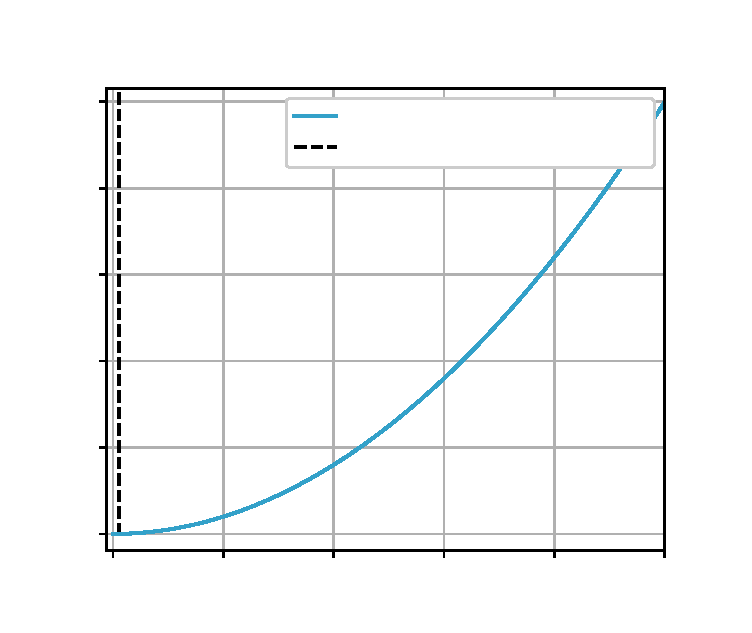
\includegraphics[width=\unitlength]{images_2ddl/eta.eps}}%
    \put(0.12494664,0.04955423){\color[rgb]{0,0,0}\makebox(0,0)[lb]{\smash{0}}}%
    \put(0.26935006,0.04955423){\color[rgb]{0,0,0}\makebox(0,0)[lb]{\smash{20}}}%
    \put(0.42297564,0.04955423){\color[rgb]{0,0,0}\makebox(0,0)[lb]{\smash{40}}}%
    \put(0.57660093,0.04955423){\color[rgb]{0,0,0}\makebox(0,0)[lb]{\smash{60}}}%
    \put(0.73022622,0.04955423){\color[rgb]{0,0,0}\makebox(0,0)[lb]{\smash{80}}}%
    \put(0.87462877,0.04955423){\color[rgb]{0,0,0}\makebox(0,0)[lb]{\smash{100}}}%
    \put(0.08654466,0.10358121){\color[rgb]{0,0,0}\makebox(0,0)[lb]{\smash{0}}}%
    \put(0.03121375,0.22391821){\color[rgb]{0,0,0}\makebox(0,0)[lb]{\smash{1000}}}%
    \put(0.03121375,0.34425464){\color[rgb]{0,0,0}\makebox(0,0)[lb]{\smash{2000}}}%
    \put(0.03121375,0.46459107){\color[rgb]{0,0,0}\makebox(0,0)[lb]{\smash{3000}}}%
    \put(0.03121375,0.58492749){\color[rgb]{0,0,0}\makebox(0,0)[lb]{\smash{4000}}}%
    \put(0.03121375,0.70526392){\color[rgb]{0,0,0}\makebox(0,0)[lb]{\smash{5000}}}%
    \put(0.46800464,0.68690835){\color[rgb]{0,0,0}\makebox(0,0)[lb]{\smash{$\eta_{max}$}}}%
    \put(0.46800464,0.64354118){\color[rgb]{0,0,0}\makebox(0,0)[lb]{\smash{\small valeur minimale de  $F/m_r g$ }}}%
    \put(0.46,0.0155423){\color[rgb]{0,0,0}\makebox(0,0)[lb]{\smash{$F/m_r g$}}}%
  \end{picture}%
\endgroup%

\caption{Variation de la hauteur maximale de saut adimensionnelle $\eta_{max}$ en fonction du ratio $F/m_r g$}
\label{fig:eta}
\end{figure}

\begin{figure}[htb]
\centering
\def\svgwidth{320}
%% Creator: Inkscape inkscape 0.92.2, www.inkscape.org
%% PDF/EPS/PS + LaTeX output extension by Johan Engelen, 2010
%% Accompanies image file 'eff.eps' (pdf, eps, ps)
%%
%% To include the image in your LaTeX document, write
%%   \input{<filename>.pdf_tex}
%%  instead of
%%   \includegraphics{<filename>.pdf}
%% To scale the image, write
%%   \def\svgwidth{<desired width>}
%%   \input{<filename>.pdf_tex}
%%  instead of
%%   \includegraphics[width=<desired width>]{<filename>.pdf}
%%
%% Images with a different path to the parent latex file can
%% be accessed with the `import' package (which may need to be
%% installed) using
%%   \usepackage{import}
%% in the preamble, and then including the image with
%%   \import{<path to file>}{<filename>.pdf_tex}
%% Alternatively, one can specify
%%   \graphicspath{{<path to file>/}}
%% 
%% For more information, please see info/svg-inkscape on CTAN:
%%   http://tug.ctan.org/tex-archive/info/svg-inkscape
%%
\begingroup%
  \makeatletter%
  \providecommand\color[2][]{%
    \errmessage{(Inkscape) Color is used for the text in Inkscape, but the package 'color.sty' is not loaded}%
    \renewcommand\color[2][]{}%
  }%
  \providecommand\transparent[1]{%
    \errmessage{(Inkscape) Transparency is used (non-zero) for the text in Inkscape, but the package 'transparent.sty' is not loaded}%
    \renewcommand\transparent[1]{}%
  }%
  \providecommand\rotatebox[2]{#2}%
  \ifx\svgwidth\undefined%
    \setlength{\unitlength}{344.79999138bp}%
    \ifx\svgscale\undefined%
      \relax%
    \else%
      \setlength{\unitlength}{\unitlength * \real{\svgscale}}%
    \fi%
  \else%
    \setlength{\unitlength}{\svgwidth}%
  \fi%
  \global\let\svgwidth\undefined%
  \global\let\svgscale\undefined%
  \makeatother%
  \begin{picture}(1,0.83526682)%
    \put(0,0){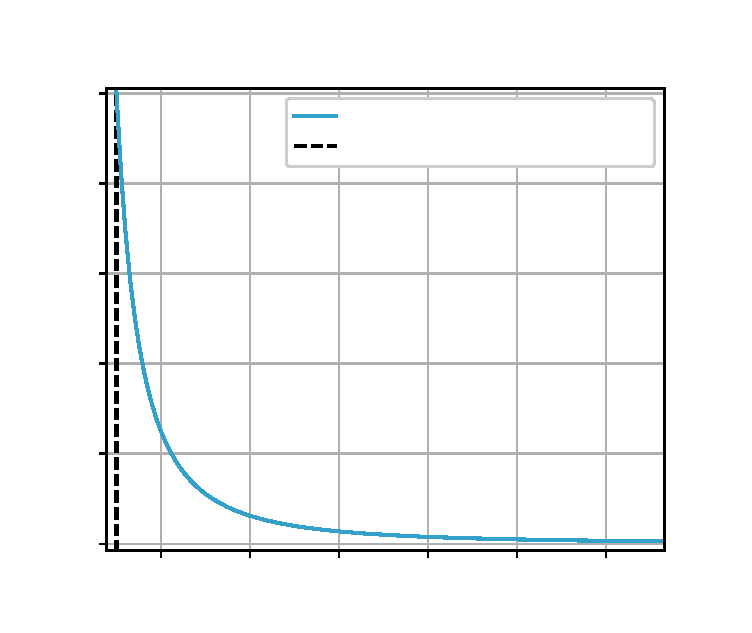
\includegraphics[width=\unitlength]{images_2ddl/eff.eps}}%
    \put(0.19169287,0.04955423){\color[rgb]{0,0,0}\makebox(0,0)[lb]{\smash{2}}}%
    \put(0.31560035,0.04955423){\color[rgb]{0,0,0}\makebox(0,0)[lb]{\smash{4}}}%
    \put(0.43950406,0.04955423){\color[rgb]{0,0,0}\makebox(0,0)[lb]{\smash{6}}}%
    \put(0.56341067,0.04955423){\color[rgb]{0,0,0}\makebox(0,0)[lb]{\smash{8}}}%
    \put(0.67809745,0.04955423){\color[rgb]{0,0,0}\makebox(0,0)[lb]{\smash{10}}}%
    \put(0.80200116,0.04955423){\color[rgb]{0,0,0}\makebox(0,0)[lb]{\smash{12}}}%
    \put(0.05885673,0.08975435){\color[rgb]{0,0,0}\makebox(0,0)[lb]{\smash{0.5}}}%
    \put(0.05885673,0.21525174){\color[rgb]{0,0,0}\makebox(0,0)[lb]{\smash{0.6}}}%
    \put(0.05885673,0.34074826){\color[rgb]{0,0,0}\makebox(0,0)[lb]{\smash{0.7}}}%
    \put(0.05885673,0.4662471){\color[rgb]{0,0,0}\makebox(0,0)[lb]{\smash{0.8}}}%
    \put(0.05885673,0.59174304){\color[rgb]{0,0,0}\makebox(0,0)[lb]{\smash{0.9}}}%
    \put(0.05885673,0.71724188){\color[rgb]{0,0,0}\makebox(0,0)[lb]{\smash{1.0}}}%
    \put(0.46800464,0.68690835){\color[rgb]{0,0,0}\makebox(0,0)[lb]{\smash{$E_{p,g}/E_{tot}$}}}%
    \put(0.46800464,0.64435615){\color[rgb]{0,0,0}\makebox(0,0)[lb]{\smash{\small valeur minimale de $F/m_r g$ }}}%
    \put(0.460200116,0.0155423){\color[rgb]{0,0,0}\makebox(0,0)[lb]{\smash{$F/m_r g$}}}%
  \end{picture}%
\endgroup%

\caption{Variation de l'efficacité énergétique en fonction du ratio $\dfrac{F}{m_r g}$}
\label{fig:effe}
\end{figure}

Remarques:

\begin{itemize}
    \item Les tracés adimensionnels permettent d'étudier une tendance globale, en s'affranchissant de la dépendance des résultats avec les autres paramètres.
    \item On identifie deux modes pour le mouvement du système: le mode de translation caractérisé par l'évolution de la position du centre de gravité donnée à l'équation \ref{eq:cdg2}
    $$\xi_{translation}(\tau)=-\frac{1}{2}\tau^2+\sqrt{(\frac{F}{m_r g})^2-1}\tau+\frac{2Rk}{m_r g}+\frac{1}{2},$$ et le mode de vibration, obtenu par la soustraction des positions des deux masses données dans l'équation \ref{eq:5a}: 
    $$\xi_{vibration}=\frac{\xi_1 - \xi_2}{2},$$ soit $$\xi_{vibration}=\frac{1}{2\sqrt{2}}\sin{(\sqrt{2}\tau)}\sqrt{(\frac{2F}{m_r g})^2-4}+\frac{1}{2}\cos{(\sqrt{2}\tau)}+\frac{2Rk}{m_r g}+\frac{1}{2}.$$
    Ces expressions illustrent ce qu'on constate en observant les figures \ref{fig:eta} et \ref{fig:effe}: plus le ratio $\dfrac{F}{m_r g}$ est important, plus les amplitudes des modes de translation et de vibration augmentent, et donc la hauteur maximale de saut $H_{max}$ et l'amplitude des vibrations augmentent toutes les deux. Ainsi l'efficacité énergétique décroît car l'énergie dissipée par vibration augmente en même temps que $H_{max}$ avec le ratio $\dfrac{F}{m_r g}$.
\end{itemize}

\subsection{Mise en évidence de différents régimes de saut}
Les résultats et conclusions des sous-sections précédentes sont synthétisés en figure \ref{fig:regime}. On différencie d'une part le régime linéaire du régime non linéaire selon la valeur du ratio $\delta/R$, où $\delta$ est la flèche imposée par la force $F$. On rappelle que la valeur limite en comportement linéaire a été fixée à $\delta/R=0.1$. Il existe également trois régimes de saut distincts, en fonction du ratio $\dfrac{F}{m_r g}$. Le premier, trivial, correspond au cas où la force appliquée ne suffit pas à soulever la roue: il n'y a pas de saut. Le passage d'un saut efficace énergétiquement à un saut peu efficace est déterminée par la dissipation d'énergie par vibration: plus la force augmente par rapport au poids de la roue, plus l'amplitude du mode de vibration augmente, et plus l'efficacité énergétique du saut décroît.


\begin{figure}[htb]
\def\svgwidth{400}
%% Creator: Inkscape inkscape 0.92.2, www.inkscape.org
%% PDF/EPS/PS + LaTeX output extension by Johan Engelen, 2010
%% Accompanies image file 'regimes1.eps' (pdf, eps, ps)
%%
%% To include the image in your LaTeX document, write
%%   \input{<filename>.pdf_tex}
%%  instead of
%%   \includegraphics{<filename>.pdf}
%% To scale the image, write
%%   \def\svgwidth{<desired width>}
%%   \input{<filename>.pdf_tex}
%%  instead of
%%   \includegraphics[width=<desired width>]{<filename>.pdf}
%%
%% Images with a different path to the parent latex file can
%% be accessed with the `import' package (which may need to be
%% installed) using
%%   \usepackage{import}
%% in the preamble, and then including the image with
%%   \import{<path to file>}{<filename>.pdf_tex}
%% Alternatively, one can specify
%%   \graphicspath{{<path to file>/}}
%% 
%% For more information, please see info/svg-inkscape on CTAN:
%%   http://tug.ctan.org/tex-archive/info/svg-inkscape
%%
\begingroup%
  \makeatletter%
  \providecommand\color[2][]{%
    \errmessage{(Inkscape) Color is used for the text in Inkscape, but the package 'color.sty' is not loaded}%
    \renewcommand\color[2][]{}%
  }%
  \providecommand\transparent[1]{%
    \errmessage{(Inkscape) Transparency is used (non-zero) for the text in Inkscape, but the package 'transparent.sty' is not loaded}%
    \renewcommand\transparent[1]{}%
  }%
  \providecommand\rotatebox[2]{#2}%
  \ifx\svgwidth\undefined%
    \setlength{\unitlength}{556.9991112bp}%
    \ifx\svgscale\undefined%
      \relax%
    \else%
      \setlength{\unitlength}{\unitlength * \real{\svgscale}}%
    \fi%
  \else%
    \setlength{\unitlength}{\svgwidth}%
  \fi%
  \global\let\svgwidth\undefined%
  \global\let\svgscale\undefined%
  \makeatother%
  \begin{picture}(1,0.59015529)%
    \put(0,0){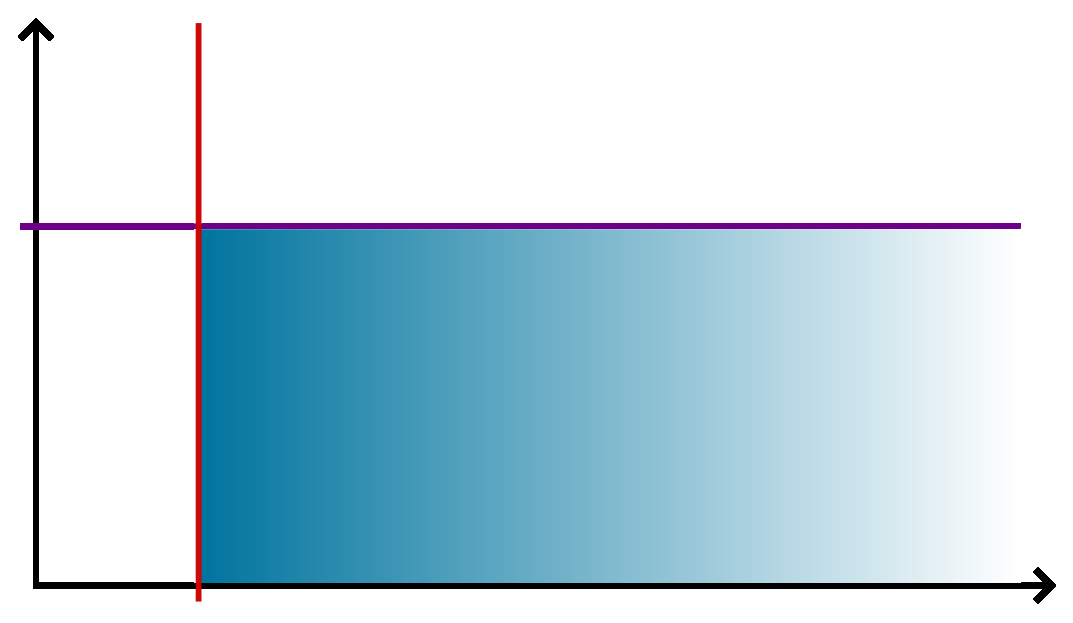
\includegraphics[width=\unitlength]{images_2ddl/regimes1.eps}}%
    \put(0.02561396,0.28811823){\color[rgb]{0,0,0}\makebox(0,0)[lb]{\smash{}}}%
    \put(0.066009,0.05921302){\color[rgb]{0,0,0}\makebox(0,0)[lb]{\smash{}}}%
    \put(-0.01,0.0){\color[rgb]{0,0,0}\makebox(0,0)[lb]{\smash{0}}}%
    \put(-0.0384028,0.35794642){\color[rgb]{0,0,0}\makebox(0,0)[lb]{\smash{0.1}}}%
    \put(0.170346148,-0.02){\color[rgb]{0,0,0}\makebox(0,0)[lb]{\smash{1}}}%
    \put(0.095137172,0.25955463){\color[rgb]{0.8,0,0}\makebox(0,0)[b]{\smash{PAS}}}%
    \put(0.095137172,0.20955463){\color[rgb]{0.8,0,0}\makebox(0,0)[b]{\smash{DE}}}%
    \put(0.095137172,0.15955463){\color[rgb]{0.8,0,0}\makebox(0,0)[b]{\smash{SAUT}}}%
    \put(0.350802717,0.23077807){\color[rgb]{0,0,0.01176471}\makebox(0,0)[b]{\smash{SAUT AVEC PEU}}}%
    \put(0.350802717,0.18077807){\color[rgb]{0,0,0.01176471}\makebox(0,0)[b]{\smash{DE VIBRATIONS}}}%
    \put(0.75539718,0.20955463){\color[rgb]{0,0,0.02745098}\makebox(0,0)[b]{\smash{SAUT  EFFICACE À 50\%}}}%
    \put(0.22758915,0.44969837){\color[rgb]{0,0,0}\makebox(0,0)[lb]{\smash{}}}%
    \put(0.58988013,0.43773024){\color[rgb]{0.43137255,0,0.53333333}\makebox(0,0)[b]{\smash{NON LINÉARITÉ GÉOMÉTRIQUE}}}%
    \put(0.0,0.59741848){\color[rgb]{0,0,0}\makebox(0,0)[lb]{\smash{$\dfrac{F}{kR}$}}}%
    \put(0.96816481,0.05921302){\color[rgb]{0,0,0}\makebox(0,0)[lb]{\smash{}}}%
    \put(1.01,0.01016188){\color[rgb]{0,0,0}\makebox(0,0)[lb]{\smash{$\dfrac{F}{m_r g}$}}}%
  \end{picture}%
\endgroup%

\caption{Carte des différents régimes de saut possibles pour une roue Cyr en fonction des ratios $F/kR$ et $F/m_r g$.}
\label{fig:regime}
\end{figure}

\subsection{Étude de $H_{max}$ en fonction de la géométrie de la section}
Nous avons vu que la rigidité $k$ et la masse $m_r$ de la roue sont des paramètres déterminants pour $H_{max}$. 
D'après \ref{eq:km1}, on peut moduler $k$ et $m_r$ en jouant sur les propriétés du matériau avec la masse volumique $\rho$ et le module de Young $E$, ou bien en jouant sur la géométrie avec le rayon médian de la roue $R$ et les rayons intérieur et extérieur de la section $r_1$, $r_2$ qui déterminent l'aire de section $A$ et le moment quadratique de section $I$.
\begin{align}
    k&=\frac{4\pi EI}{(\pi^2 -8)R^3} &  I&=\frac{\pi}{4}(r_2^4-r_1^4) \nonumber\\
    m_r&=2\pi R \rho A   & A&=\pi (r_2^2-r_1^2)
    \label{eq:km1}
\end{align}

Les dimensions de la section, caractérisées par $r_1$ et $r_2$, sont les paramètres les plus malléables. Nous allons étudier leur influence sur la hauteur maximale de saut puis en déduire des valeurs optimisées. \\
Le matériau considéré dans cette étude sera le matériau ayant le module de Young le plus élevé parmi ceux disponibles pour l'imprimante 3D utilisée.\\
Il s'agit du nylon renforcé avec des fibres de carbone courtes, ayant pour masse volumique $\rho=1170 kg \cdot m^{-3}$, pour module d'Young $E=9.0 GPa$, pour module de cisaillement $G=3.8 GPa$ et une contrainte à la rupture $\sigma_r=63.0 MPa$.\\
Le rayon médian $R$ de la roue sera compris entre $0.8 m$ et $1.0 m$, nous fixons sa valeur à $0.9 m$. \\
On considère deux types de chargement pour la force de compression $F$ appliquée au sommet de la roue: 
\begin{itemize}
    \item $F_1=900 N$, qui correspond au cas où l'utilisateur se suspend par une main à la roue, la charge maximum qu'il peut appliquer en statique. 
    \item $F_2=c_d F_1 $, où $c_d=5$ rend compte des effets dynamiques. Le choix de la valeur de $c_d$ est basé sur des articles traitant des efforts dynamiques à l'impact exercés par des gymnastes lors de mouvements acrobatiques \cite{marinsek},\cite{seegmiller_ground_nodate}, \cite{mcnair_normative_1999},\cite{prapavessis_effects_1999} et sur les travaux de Marion Cossin, mesurant les efforts exercés par des circassiens suspendus à des agrès aériens \cite{cossin_mesure_nodate}.
\end{itemize}
 

$H_{max}$ décroît avec $k$ et $m_r$ selon les lois modélisées dans les sections précédentes. Maximiser $H_{max}$ en jouant sur les paramètres $r_1$ et $r_2$ revient à minimiser les valeurs de $I$ et de $A$, et donc réduire l'épaisseur de section. \\
La première étape qui s'impose est de définir des limites inférieures de l'épaisseur de section pour s'assurer que la roue ne sera ni sujette à du flambement, de l'écoulement et qu'on restera dans le domaine de comportement linéaire.
Dans ce qui suit pour chaque valeur fixe du rayon externe $r_2$, comprise entre $10 mm$ et $50 mm$, nous étudierons le comportement de la roue pour un rayon interne $r_1$ variant de $0 mm$ à $r_2 - 0.01 mm$.

\subsubsection{Limites en flambement et en écoulement lors de la compression}

Lorsqu'on exerce une force de compression au sommet de la roue, des phénomènes de flambement et d'écoulement apparaissent si sa section n'est pas assez épaisse. 
Pour chaque valeur du rayon externe $r_2$, compris entre $10 mm$ et $50 mm$, on cherche à savoir quelle est la valeur maximale du rayon interne $r_1$ permettant d'éviter ces phénomènes. 

 \begin{figure}[h]
\centering
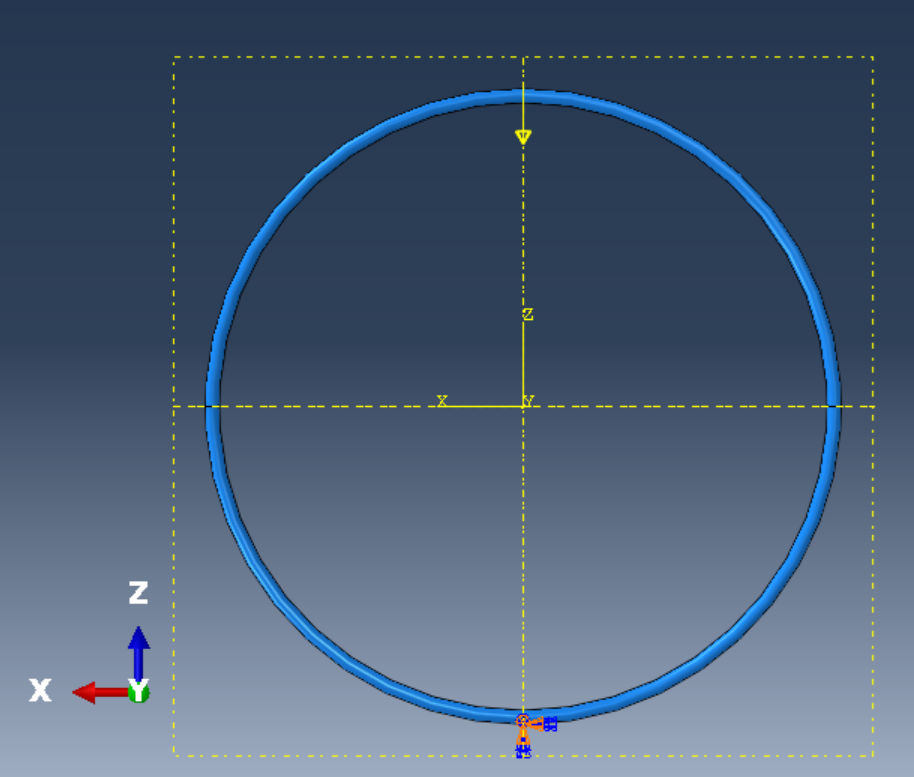
\includegraphics[width=200]{saut2/elf1.PNG}
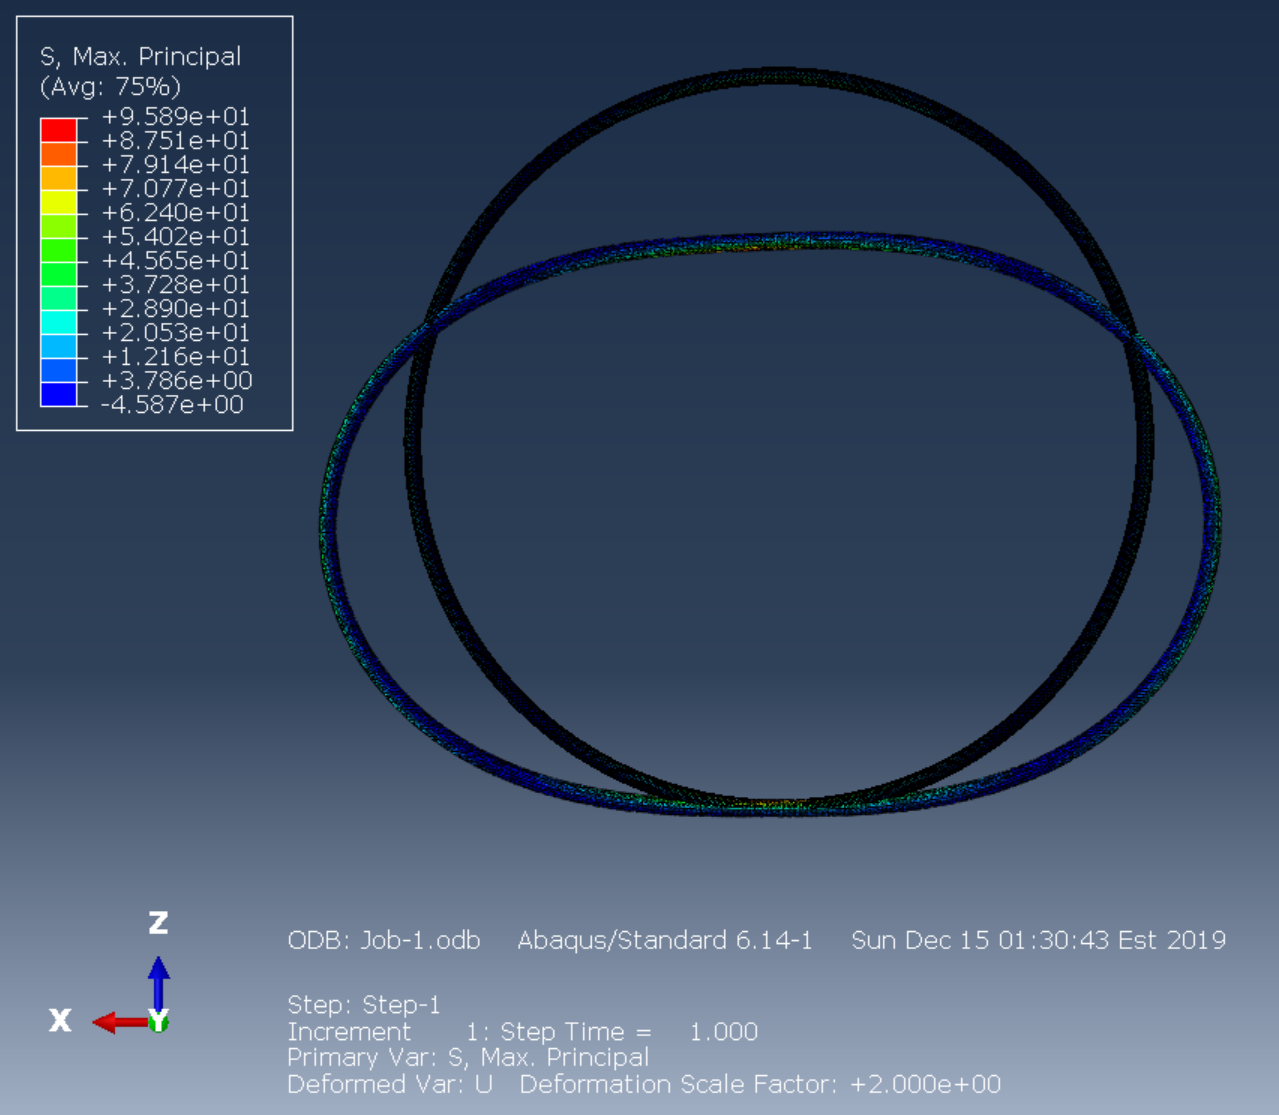
\includegraphics[width=241]{saut2/elf2.PNG}
\caption{Modélisation éléments finis d'une roue Cyr comprimée par une force exercée à son sommet.}
\label{fig:elf1}
\end{figure}

Pour chaque valeur du rayon externe $r_2$, compris entre $10 mm$ et $50 mm$, une étude linéaire par éléments finis nous donne le rayon interne $r_1$ à partir duquel il y a flambement dans la roue. 
De même manière, une étude linéaire des contraintes dans la roue par éléments finis nous donne pour chaque $r_2$, le $r_1$ à partir duquel il y a écoulement. 

On combine ces deux études: pour chaque $r_2$, on ajuste $r_1$ jusqu'à ce qu'il y ait flambement et écoulement en même temps, c'est à dire jusqu'au moment où la différence de chargement qui provoque chacun de ces deux phénomènes atteint sa valeur minimale (figure \ref{fig:fle12}). 
 \begin{figure}[h]
\centering
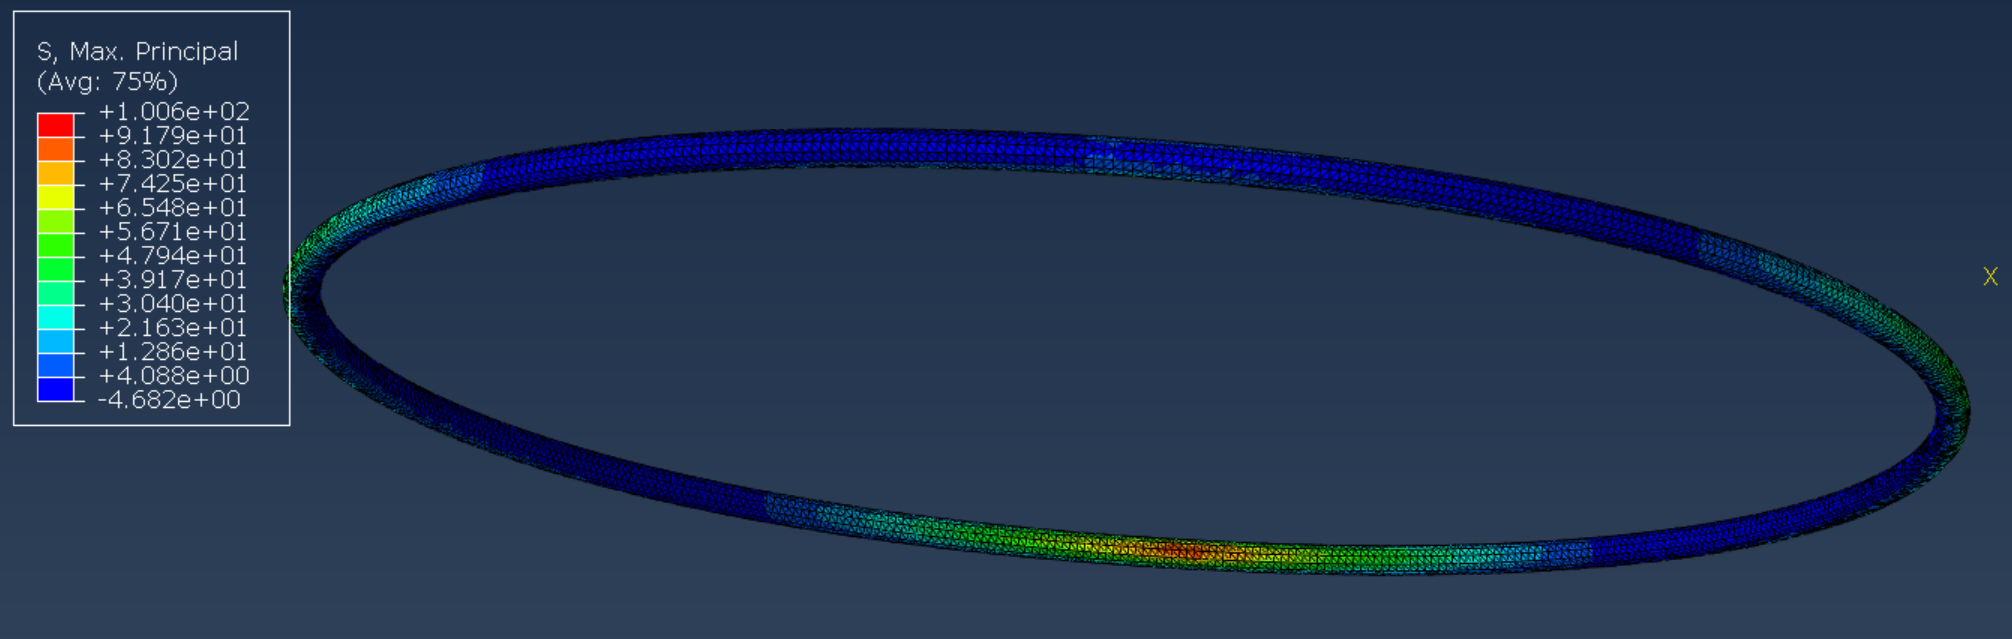
\includegraphics[width=400]{saut2/elf3.PNG}
\caption{Contraintes dans la roue lors de la compression par une force exercée à son sommet, obtenues par une analyse éléments finis linéaire. Les contraintes maximales se situent au niveau du rayon interne de la roue là où la force est exercée et dans la zone diamétralement opposée à cet endroit.}
\label{fig:elf2}
\end{figure}

Les paramètres des études éléments finis correspondent à une roue de rayon médian $R=0.9 m$, en nylon renforcé avec des fibres de carbone courtes à laquelle on applique la force de compression $F=F_2$.

\begin{figure}[h]
\def\svgwidth{240}
%% Creator: Inkscape inkscape 0.92.2, www.inkscape.org
%% PDF/EPS/PS + LaTeX output extension by Johan Engelen, 2010
%% Accompanies image file 'fle1.eps' (pdf, eps, ps)
%%
%% To include the image in your LaTeX document, write
%%   \input{<filename>.pdf_tex}
%%  instead of
%%   \includegraphics{<filename>.pdf}
%% To scale the image, write
%%   \def\svgwidth{<desired width>}
%%   \input{<filename>.pdf_tex}
%%  instead of
%%   \includegraphics[width=<desired width>]{<filename>.pdf}
%%
%% Images with a different path to the parent latex file can
%% be accessed with the `import' package (which may need to be
%% installed) using
%%   \usepackage{import}
%% in the preamble, and then including the image with
%%   \import{<path to file>}{<filename>.pdf_tex}
%% Alternatively, one can specify
%%   \graphicspath{{<path to file>/}}
%% 
%% For more information, please see info/svg-inkscape on CTAN:
%%   http://tug.ctan.org/tex-archive/info/svg-inkscape
%%
\begingroup%
  \makeatletter%
  \providecommand\color[2][]{%
    \errmessage{(Inkscape) Color is used for the text in Inkscape, but the package 'color.sty' is not loaded}%
    \renewcommand\color[2][]{}%
  }%
  \providecommand\transparent[1]{%
    \errmessage{(Inkscape) Transparency is used (non-zero) for the text in Inkscape, but the package 'transparent.sty' is not loaded}%
    \renewcommand\transparent[1]{}%
  }%
  \providecommand\rotatebox[2]{#2}%
  \ifx\svgwidth\undefined%
    \setlength{\unitlength}{344.79999138bp}%
    \ifx\svgscale\undefined%
      \relax%
    \else%
      \setlength{\unitlength}{\unitlength * \real{\svgscale}}%
    \fi%
  \else%
    \setlength{\unitlength}{\svgwidth}%
  \fi%
  \global\let\svgwidth\undefined%
  \global\let\svgscale\undefined%
  \makeatother%
  \begin{picture}(1,0.83526682)%
    \put(0,0){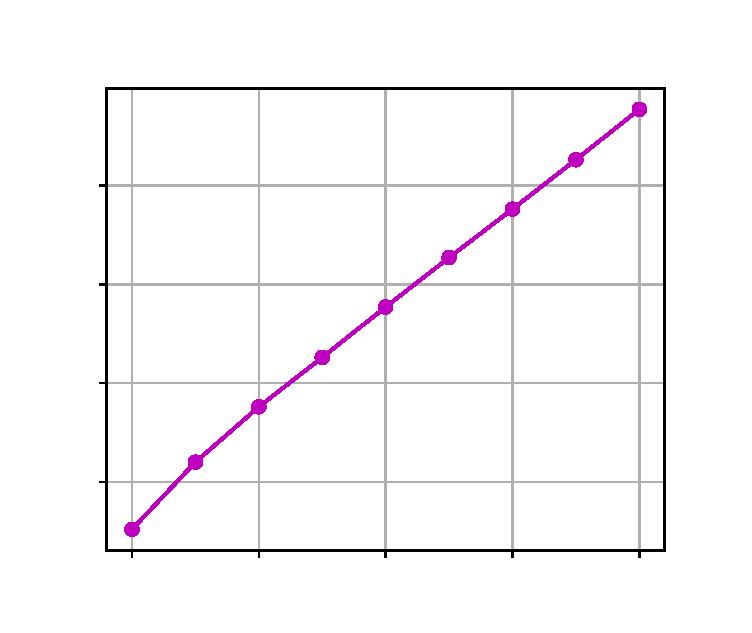
\includegraphics[width=\unitlength]{images_2ddl/fle1.eps}}%
    \put(0.14215545,0.044955423){\color[rgb]{0,0,0}\makebox(0,0)[lb]{\smash{10}}}%
    \put(0.3187007,0.044955423){\color[rgb]{0,0,0}\makebox(0,0)[lb]{\smash{20}}}%
    \put(0.49524652,0.044955423){\color[rgb]{0,0,0}\makebox(0,0)[lb]{\smash{30}}}%
    \put(0.67178944,0.044955423){\color[rgb]{0,0,0}\makebox(0,0)[lb]{\smash{40}}}%
    \put(0.84833527,0.044955423){\color[rgb]{0,0,0}\makebox(0,0)[lb]{\smash{50}}}%
    \put(0.056810122,0.17613689){\color[rgb]{0,0,0}\makebox(0,0)[lb]{\smash{10}}}%
    \put(0.056810122,0.3137094){\color[rgb]{0,0,0}\makebox(0,0)[lb]{\smash{20}}}%
    \put(0.056810122,0.4512848){\color[rgb]{0,0,0}\makebox(0,0)[lb]{\smash{30}}}%
    \put(0.056810122,0.58885731){\color[rgb]{0,0,0}\makebox(0,0)[lb]{\smash{40}}}%
    \put(0.025047303,0.31404872){\color[rgb]{0,0,0}\rotatebox{90}{\makebox(0,0)[lb]{\smash{$r_1 (mm)$}}}}%
    \put(0.45,0.0){\color[rgb]{0,0,0}\makebox(0,0)[lb]{\smash{$r_2 (mm)$}}}%
  \end{picture}%
\endgroup%

\def\svgwidth{240}
%% Creator: Inkscape inkscape 0.92.2, www.inkscape.org
%% PDF/EPS/PS + LaTeX output extension by Johan Engelen, 2010
%% Accompanies image file 'fle2.eps' (pdf, eps, ps)
%%
%% To include the image in your LaTeX document, write
%%   \input{<filename>.pdf_tex}
%%  instead of
%%   \includegraphics{<filename>.pdf}
%% To scale the image, write
%%   \def\svgwidth{<desired width>}
%%   \input{<filename>.pdf_tex}
%%  instead of
%%   \includegraphics[width=<desired width>]{<filename>.pdf}
%%
%% Images with a different path to the parent latex file can
%% be accessed with the `import' package (which may need to be
%% installed) using
%%   \usepackage{import}
%% in the preamble, and then including the image with
%%   \import{<path to file>}{<filename>.pdf_tex}
%% Alternatively, one can specify
%%   \graphicspath{{<path to file>/}}
%% 
%% For more information, please see info/svg-inkscape on CTAN:
%%   http://tug.ctan.org/tex-archive/info/svg-inkscape
%%
\begingroup%
  \makeatletter%
  \providecommand\color[2][]{%
    \errmessage{(Inkscape) Color is used for the text in Inkscape, but the package 'color.sty' is not loaded}%
    \renewcommand\color[2][]{}%
  }%
  \providecommand\transparent[1]{%
    \errmessage{(Inkscape) Transparency is used (non-zero) for the text in Inkscape, but the package 'transparent.sty' is not loaded}%
    \renewcommand\transparent[1]{}%
  }%
  \providecommand\rotatebox[2]{#2}%
  \ifx\svgwidth\undefined%
    \setlength{\unitlength}{344.79999138bp}%
    \ifx\svgscale\undefined%
      \relax%
    \else%
      \setlength{\unitlength}{\unitlength * \real{\svgscale}}%
    \fi%
  \else%
    \setlength{\unitlength}{\svgwidth}%
  \fi%
  \global\let\svgwidth\undefined%
  \global\let\svgscale\undefined%
  \makeatother%
  \begin{picture}(1,0.83526682)%
    \put(0,0){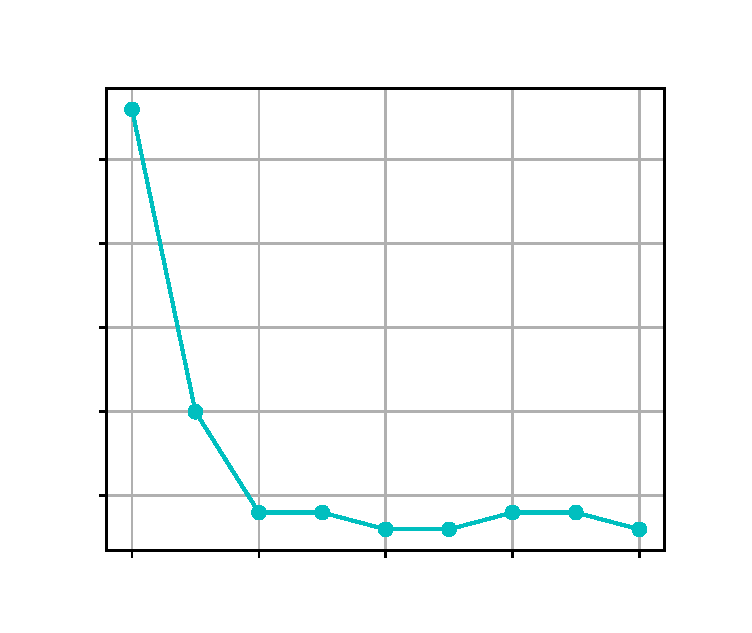
\includegraphics[width=\unitlength]{images_2ddl/fle2.eps}}%
    \put(0.14215545,0.044955423){\color[rgb]{0,0,0}\makebox(0,0)[lb]{\smash{10}}}%
    \put(0.3187007,0.044955423){\color[rgb]{0,0,0}\makebox(0,0)[lb]{\smash{20}}}%
    \put(0.49524652,0.044955423){\color[rgb]{0,0,0}\makebox(0,0)[lb]{\smash{30}}}%
    \put(0.67178944,0.044955423){\color[rgb]{0,0,0}\makebox(0,0)[lb]{\smash{40}}}%
    \put(0.84833527,0.044955423){\color[rgb]{0,0,0}\makebox(0,0)[lb]{\smash{50}}}%
    \put(0.045885673,0.15687645){\color[rgb]{0,0,0}\makebox(0,0)[lb]{\smash{2.5}}}%
    \put(0.045885673,0.27381352){\color[rgb]{0,0,0}\makebox(0,0)[lb]{\smash{3.0}}}%
    \put(0.045885673,0.39075116){\color[rgb]{0,0,0}\makebox(0,0)[lb]{\smash{3.5}}}%
    \put(0.045885673,0.50768852){\color[rgb]{0,0,0}\makebox(0,0)[lb]{\smash{4.0}}}%
    \put(0.045885673,0.62462587){\color[rgb]{0,0,0}\makebox(0,0)[lb]{\smash{4.5}}}%
    
    \put(0.49524652,0.0){\color[rgb]{0,0,0}\makebox(0,0)[lb]{\smash{$r_2 (mm)$}}}%
    \put(0.025,0.25896752){\color[rgb]{0,0,0}\rotatebox{90}{\makebox(0,0)[lb]{\smash{épaisseur $(mm)$}}}}%
  \end{picture}%
\endgroup%

\caption{Couples $(r_1,r_2)$ pour lesquels on à a la fois flambement et écoulement dans la roue en nylon renforcé aux fibres de carbone courtes, pour une force $F_2=4500 N$ appliquée à son sommet.}
\label{fig:fle12}
\end{figure}

\subsubsection{Limites en écoulement à l'impact}

Lorsque l'utilisateur saute avec la roue, la partie entre ses pieds et le sol est soumise à des contraintes dues à l'impact de l'atterrissage qui créent de l'écoulement et un écrasement de la section si son épaisseur n'est pas suffisante. 

Le saut peut s'effectuer pieds joints ou écartés. La configuration pieds joints étant celle qui génère le plus de contraintes, c'est la seule que nous étudierons.

De même que précédemment, pour chaque valeur du rayon externe $r_2$, compris entre $10 mm$ et $50 mm$, une étude linéaire par éléments finis nous donne le rayon interne $r_1$ à partir duquel il y a écoulement dans la section. \\
Pour cette étude, on modélise uniquement la partie inférieure de la roue, qu'on approxime par un cylindre auquel est appliqué la pression correspondant à la force $F_2$ répartie sur la surface de contact entre les pieds de l'utilisateur et la roue (figure \ref{fig:ecrasement}).

 \begin{figure}[h]
\centering
\includegraphics[width=290]{saut2/elf4.PNG}
\includegraphics[width=170]{saut2/elf5.PNG}
\caption{Modélisation éléments finis de l'écrasement de la section de la roue entre les pieds de l'utilisateur et le sol lors de l'impact dû à l'atterrissage.}
\label{fig:ecrasement}
\end{figure}

\subsubsection{Limites en comportement linéaire}
Pour rester dans le domaine de comportement linéaire géométrique défini au début du chapitre la flèche $\delta$ imposée par l'utilisateur ne doit pas dépasser 10\% du rayon médian $R$. 
Cette condition s'applique au cas d'utilisation courant de la roue, le chargement correspondant est la force $F_1$.
On évalue la flèche avec son expression théorique: $\delta=F_1/k$, où $k$ est la constante élastique définie plus haut, pour une roue en nylon renforcé aux fibres de carbone courtes de rayon médian $R=0.9 m$. 
Pour chaque $r_2$ donné, on obtient ainsi la valeur maximale de $r_1$ pour rester dans le domaine linéaire (figure \ref{fig:fle4}). On remarque que pour $r_2=10 mm$ il n'est pas possible d'avoir un comportement linéaire, la courbe se trouvant entièrement au delà de la frontière. On éliminera donc le cas $r_2=10 mm$ pour la suite.

\begin{figure}
\centering
\def\svgwidth{350}
%% Creator: Inkscape inkscape 0.92.2, www.inkscape.org
%% PDF/EPS/PS + LaTeX output extension by Johan Engelen, 2010
%% Accompanies image file 'fle4.eps' (pdf, eps, ps)
%%
%% To include the image in your LaTeX document, write
%%   \input{<filename>.pdf_tex}
%%  instead of
%%   \includegraphics{<filename>.pdf}
%% To scale the image, write
%%   \def\svgwidth{<desired width>}
%%   \input{<filename>.pdf_tex}
%%  instead of
%%   \includegraphics[width=<desired width>]{<filename>.pdf}
%%
%% Images with a different path to the parent latex file can
%% be accessed with the `import' package (which may need to be
%% installed) using
%%   \usepackage{import}
%% in the preamble, and then including the image with
%%   \import{<path to file>}{<filename>.pdf_tex}
%% Alternatively, one can specify
%%   \graphicspath{{<path to file>/}}
%% 
%% For more information, please see info/svg-inkscape on CTAN:
%%   http://tug.ctan.org/tex-archive/info/svg-inkscape
%%
\begingroup%
  \makeatletter%
  \providecommand\color[2][]{%
    \errmessage{(Inkscape) Color is used for the text in Inkscape, but the package 'color.sty' is not loaded}%
    \renewcommand\color[2][]{}%
  }%
  \providecommand\transparent[1]{%
    \errmessage{(Inkscape) Transparency is used (non-zero) for the text in Inkscape, but the package 'transparent.sty' is not loaded}%
    \renewcommand\transparent[1]{}%
  }%
  \providecommand\rotatebox[2]{#2}%
  \ifx\svgwidth\undefined%
    \setlength{\unitlength}{632.22074835bp}%
    \ifx\svgscale\undefined%
      \relax%
    \else%
      \setlength{\unitlength}{\unitlength * \real{\svgscale}}%
    \fi%
  \else%
    \setlength{\unitlength}{\svgwidth}%
  \fi%
  \global\let\svgwidth\undefined%
  \global\let\svgscale\undefined%
  \makeatother%
  \begin{picture}(1,0.45553708)%
    \put(0,0){\includegraphics[width=\unitlength]{images_2ddl/fle4.eps}}%
    \put(0.12,0.02702584){\color[rgb]{0,0,0}\makebox(0,0)[lb]{\smash{0}}}%
    \put(0.26,0.02702584){\color[rgb]{0,0,0}\makebox(0,0)[lb]{\smash{10}}}%
    \put(0.41,0.02702584){\color[rgb]{0,0,0}\makebox(0,0)[lb]{\smash{20}}}%
    \put(0.56,0.02702584){\color[rgb]{0,0,0}\makebox(0,0)[lb]{\smash{30}}}%
    \put(0.71,0.02702584){\color[rgb]{0,0,0}\makebox(0,0)[lb]{\smash{40}}}%
    \put(0.86,0.02702584){\color[rgb]{0,0,0}\makebox(0,0)[lb]{\smash{50}}}%
    \put(0.06,0.1){\color[rgb]{0,0,0}\makebox(0,0)[lb]{\smash{0.0}}}%
    \put(0.06,0.165){\color[rgb]{0,0,0}\makebox(0,0)[lb]{\smash{0.1}}}%
    \put(0.06,0.23){\color[rgb]{0,0,0}\makebox(0,0)[lb]{\smash{0.2}}}%
    \put(0.06,0.3){\color[rgb]{0,0,0}\makebox(0,0)[lb]{\smash{0.3}}}%
    \put(0.06,0.365){\color[rgb]{0,0,0}\makebox(0,0)[lb]{\smash{0.4}}}%
    \put(0.06,0.435){\color[rgb]{0,0,0}\makebox(0,0)[lb]{\smash{0.5}}}%
    \put(0.06,0.5){\color[rgb]{0,0,0}\makebox(0,0)[lb]{\smash{0.6}}}%
    \put(0.06,0.565){\color[rgb]{0,0,0}\makebox(0,0)[lb]{\smash{0.7}}}%
    \put(0.03,0.3){\color[rgb]{0,0,0}\rotatebox{90}{\makebox(0,0)[lb]{\smash{$\delta / R$}}}}%
    \put(0.445,0.0){\color[rgb]{0,0,0}\makebox(0,0)[lb]{\smash{$r_1(mm)$}}}%
    \put(0.74,0.55){\color[rgb]{0,0,0}\makebox(0,0)[lb]{\smash{\footnotesize $r_2=10 mm$}}}%
    \put(0.74,0.515){\color[rgb]{0,0,0}\makebox(0,0)[lb]{\smash{\footnotesize $r_2=15 mm$}}}%
    \put(0.74,0.48){\color[rgb]{0,0,0}\makebox(0,0)[lb]{\smash{\footnotesize $r_2=20 mm$}}}%
    \put(0.74,0.445){\color[rgb]{0,0,0}\makebox(0,0)[lb]{\smash{\footnotesize $r_2=25 mm$}}}%
    \put(0.74,0.413){\color[rgb]{0,0,0}\makebox(0,0)[lb]{\smash{\footnotesize $r_2=30 mm$}}}%
    \put(0.74,0.38){\color[rgb]{0,0,0}\makebox(0,0)[lb]{\smash{\footnotesize $r_2=35 mm$}}}%
    \put(0.74,0.345){\color[rgb]{0,0,0}\makebox(0,0)[lb]{\smash{\footnotesize $r_2=40 mm$}}}%
    \put(0.74,0.31){\color[rgb]{0,0,0}\makebox(0,0)[lb]{\smash{\footnotesize $r_2=45 mm$}}}%
    \put(0.74,0.275){\color[rgb]{0,0,0}\makebox(0,0)[lb]{\smash{\footnotesize $r_2=50 mm$}}}%
  \end{picture}%
\endgroup%

\caption{Ratio $\delta/R$ en fonction de $r_1$ pour un $r_2$ donné. La droite horizontale en pointillés correspond à la valeur $0.1$ au delà de laquelle on quitte le domaine de comportement linéaire. L'intersection de cette droite avec chacune des courbes donne la valeur de $r_1$ à ne pas dépasser pour rester dans le domaine linéaire géométrique. Les calculs sont réalisés pour une roue en nylon renforcé aux fibres de carbone courtes de rayon médian $R=0.9 m$, avec une force $F_1=900N$ appliquée à son sommet.}
\label{fig:fle4}
\end{figure}

\subsubsection{Optimisation de la section pour le saut de la roue Cyr}
Les limites obtenues dans les trois sections précédentes sont combinées à l'étude de la hauteur maximale de saut en fonction de $r_1$, pour chaque $r_2$ compris entre $15 mm$ et $50 mm$ (figure \ref{fig:fle3}). On estime la hauteur de saut avec notre modèle à deux degrés de liberté en considérant que la roue est comprimée d'une force de $900N$ puis relâchée. Par exemple, pour $r_2=15 mm$ on obtient des sauts de plusieurs mètres lorsque $r_1$ avoisine les $14mm$, cependant on sortira de la zone de comportement linéaire, la roue sera sujette au flambement et à l'écoulement lors de sa compression et il y aura écrasement de section à l'impact lors des sauts. Pour chaque courbe, les points d'intersection avec chacune des trois limites de $r_1$ correspondent aux hauteurs de saut optimisées pour chaque type de limite.


\begin{figure}[h]
\centering
\def\svgwidth{500}
%% Creator: Inkscape inkscape 0.92.2, www.inkscape.org
%% PDF/EPS/PS + LaTeX output extension by Johan Engelen, 2010
%% Accompanies image file 'fle3.eps' (pdf, eps, ps)
%%
%% To include the image in your LaTeX document, write
%%   \input{<filename>.pdf_tex}
%%  instead of
%%   \includegraphics{<filename>.pdf}
%% To scale the image, write
%%   \def\svgwidth{<desired width>}
%%   \input{<filename>.pdf_tex}
%%  instead of
%%   \includegraphics[width=<desired width>]{<filename>.pdf}
%%
%% Images with a different path to the parent latex file can
%% be accessed with the `import' package (which may need to be
%% installed) using
%%   \usepackage{import}
%% in the preamble, and then including the image with
%%   \import{<path to file>}{<filename>.pdf_tex}
%% Alternatively, one can specify
%%   \graphicspath{{<path to file>/}}
%% 
%% For more information, please see info/svg-inkscape on CTAN:
%%   http://tug.ctan.org/tex-archive/info/svg-inkscape
%%
\begingroup%
  \makeatletter%
  \providecommand\color[2][]{%
    \errmessage{(Inkscape) Color is used for the text in Inkscape, but the package 'color.sty' is not loaded}%
    \renewcommand\color[2][]{}%
  }%
  \providecommand\transparent[1]{%
    \errmessage{(Inkscape) Transparency is used (non-zero) for the text in Inkscape, but the package 'transparent.sty' is not loaded}%
    \renewcommand\transparent[1]{}%
  }%
  \providecommand\rotatebox[2]{#2}%
  \ifx\svgwidth\undefined%
    \setlength{\unitlength}{575.9999856bp}%
    \ifx\svgscale\undefined%
      \relax%
    \else%
      \setlength{\unitlength}{\unitlength * \real{\svgscale}}%
    \fi%
  \else%
    \setlength{\unitlength}{\svgwidth}%
  \fi%
  \global\let\svgwidth\undefined%
  \global\let\svgscale\undefined%
  \makeatother%
  \begin{picture}(1,0.66111111)%
    \put(0,0){\includegraphics[width=\unitlength]{images_2ddl/fle3.eps}}%
    \put(0.12102726,0.04753889){\color[rgb]{0,0,0}\makebox(0,0)[lb]{\smash{0}}}%
    \put(0.26804688,0.04753889){\color[rgb]{0,0,0}\makebox(0,0)[lb]{\smash{10}}}%
    \put(0.42058854,0.04753889){\color[rgb]{0,0,0}\makebox(0,0)[lb]{\smash{20}}}%
    \put(0.57312847,0.04753889){\color[rgb]{0,0,0}\makebox(0,0)[lb]{\smash{30}}}%
    \put(0.7256684,0.04753889){\color[rgb]{0,0,0}\makebox(0,0)[lb]{\smash{40}}}%
    \put(0.87821007,0.04753889){\color[rgb]{0,0,0}\makebox(0,0)[lb]{\smash{50}}}%
    \put(0.1018066,0.08574358){\color[rgb]{0,0,0}\makebox(0,0)[lb]{\smash{0}}}%
    \put(0.1018066,0.16424358){\color[rgb]{0,0,0}\makebox(0,0)[lb]{\smash{2}}}%
    \put(0.1018066,0.24274306){\color[rgb]{0,0,0}\makebox(0,0)[lb]{\smash{4}}}%
    \put(0.1018066,0.32124306){\color[rgb]{0,0,0}\makebox(0,0)[lb]{\smash{6}}}%
    \put(0.1018066,0.39974306){\color[rgb]{0,0,0}\makebox(0,0)[lb]{\smash{8}}}%
    \put(0.09076615,0.47824306){\color[rgb]{0,0,0}\makebox(0,0)[lb]{\smash{10}}}%
    \put(0.09076615,0.55674132){\color[rgb]{0,0,0}\makebox(0,0)[lb]{\smash{12}}}%
    \put(0.07972552,0.28014063){\color[rgb]{0,0,0}\rotatebox{90}{\makebox(0,0)[lb]{\smash{$H_{max} (m)$}}}}%
    \put(0.47221181,0.55419097){\color[rgb]{0,0,0}\makebox(0,0)[lb]{\smash{$r_2=15 mm$}}}%
    \put(0.47221181,0.52872049){\color[rgb]{0,0,0}\makebox(0,0)[lb]{\smash{$r_2=20 mm$}}}%
    \put(0.47221181,0.50324826){\color[rgb]{0,0,0}\makebox(0,0)[lb]{\smash{$r_2=25 mm$}}}%
    \put(0.47221181,0.47777604){\color[rgb]{0,0,0}\makebox(0,0)[lb]{\smash{$r_2=35 mm$}}}%
    \put(0.47221181,0.45230382){\color[rgb]{0,0,0}\makebox(0,0)[lb]{\smash{$r_2=50 mm$}}}%
    \put(0.47221181,0.4268316){\color[rgb]{0,0,0}\makebox(0,0)[lb]{\smash{limite en flambement/écoulement}}}%
    \put(0.47221181,0.40065451){\color[rgb]{0,0,0}\makebox(0,0)[lb]{\smash{$\delta / R>0.1$}}}%
    \put(0.47221181,0.37447743){\color[rgb]{0,0,0}\makebox(0,0)[lb]{\smash{limite en écoulement saut pieds joints}}}%
    \put(0.475,0.02){\color[rgb]{0,0,0}\makebox(0,0)[lb]{\smash{$r_1(mm)$}}}%
  \end{picture}%
\endgroup%

\caption{Hauteur maximale de saut en fonction de $r_1$, pour des $r_2$ donnés. Les points d'intersection des courbes $H_{max}=f(r_1)$ avec les limites en pointillés correspondent aux valeurs pour lesquelles le saut de la roue est optimisé. Les calculs sont réalisés pour une roue en nylon renforcé aux fibres de carbone courtes de rayon médian $R=0.9 m$, avec la force $F_1$ appliquée à son sommet.}
\label{fig:fle3}
\end{figure}

Ces points d'intersections reliés donnent trois nouvelles courbes correspondant chacune à un type de limite: flambement-écoulement en compression, écoulement à l'impact, sortie du domaine géométrique linéaire (figure \ref{fig:fle51}). Pour chaque $r_2$, le point le plus à gauche donne la valeur optimale de $r_1$, permettant d'avoir une épaisseur de section aussi fine que possible et de maximiser $H_{max}$ sans dommages, en gardant un comportement linéaire.

\begin{figure}[h]
\centering
\def\svgwidth{450}
%% Creator: Inkscape inkscape 0.92.2, www.inkscape.org
%% PDF/EPS/PS + LaTeX output extension by Johan Engelen, 2010
%% Accompanies image file 'fle41.eps' (pdf, eps, ps)
%%
%% To include the image in your LaTeX document, write
%%   \input{<filename>.pdf_tex}
%%  instead of
%%   \includegraphics{<filename>.pdf}
%% To scale the image, write
%%   \def\svgwidth{<desired width>}
%%   \input{<filename>.pdf_tex}
%%  instead of
%%   \includegraphics[width=<desired width>]{<filename>.pdf}
%%
%% Images with a different path to the parent latex file can
%% be accessed with the `import' package (which may need to be
%% installed) using
%%   \usepackage{import}
%% in the preamble, and then including the image with
%%   \import{<path to file>}{<filename>.pdf_tex}
%% Alternatively, one can specify
%%   \graphicspath{{<path to file>/}}
%% 
%% For more information, please see info/svg-inkscape on CTAN:
%%   http://tug.ctan.org/tex-archive/info/svg-inkscape
%%
\begingroup%
  \makeatletter%
  \providecommand\color[2][]{%
    \errmessage{(Inkscape) Color is used for the text in Inkscape, but the package 'color.sty' is not loaded}%
    \renewcommand\color[2][]{}%
  }%
  \providecommand\transparent[1]{%
    \errmessage{(Inkscape) Transparency is used (non-zero) for the text in Inkscape, but the package 'transparent.sty' is not loaded}%
    \renewcommand\transparent[1]{}%
  }%
  \providecommand\rotatebox[2]{#2}%
  \ifx\svgwidth\undefined%
    \setlength{\unitlength}{602.31990694bp}%
    \ifx\svgscale\undefined%
      \relax%
    \else%
      \setlength{\unitlength}{\unitlength * \real{\svgscale}}%
    \fi%
  \else%
    \setlength{\unitlength}{\svgwidth}%
  \fi%
  \global\let\svgwidth\undefined%
  \global\let\svgscale\undefined%
  \makeatother%
  \begin{picture}(1,0.56554637)%
    \put(0,0){\includegraphics[width=\unitlength]{images_2ddl/fle41.eps}}%
    \put(0.20661598,0.03809743){\color[rgb]{0,0,0}\makebox(0,0)[lb]{\smash{10}}}%
    \put(0.36902801,0.03809743){\color[rgb]{0,0,0}\makebox(0,0)[lb]{\smash{20}}}%
    \put(0.53144004,0.03809743){\color[rgb]{0,0,0}\makebox(0,0)[lb]{\smash{30}}}%
    \put(0.69385207,0.03809743){\color[rgb]{0,0,0}\makebox(0,0)[lb]{\smash{40}}}%
    \put(0.85626575,0.03809743){\color[rgb]{0,0,0}\makebox(0,0)[lb]{\smash{50}}}%
    \put(0.067359896,0.09206078){\color[rgb]{0,0,0}\makebox(0,0)[lb]{\smash{$10^{-2}$}}}%
    \put(0.067359896,0.21808816){\color[rgb]{0,0,0}\makebox(0,0)[lb]{\smash{$10^{-1}$}}}%
    \put(0.078356045,0.34548557){\color[rgb]{0,0,0}\makebox(0,0)[lb]{\smash{$10^0$}}}%
    \put(0.078356045,0.47151162){\color[rgb]{0,0,0}\makebox(0,0)[lb]{\smash{$10^1$}}}%
    \put(0.06304079,0.23476368){\color[rgb]{0,0,0}\rotatebox{90}{\makebox(0,0)[lb]{\smash{$H_{ma x}(m)$}}}}%
    \put(0.5,0.01){\color[rgb]{0,0,0}\makebox(0,0)[lb]{\smash{$r_1 (mm)$}}}%
    \put(0.188649545,0.25123168){\color[rgb]{0,0,0}\makebox(0,0)[lb]{\smash{\scriptsize flambement/écoulement}}}%
    \put(0.18649545,0.22687253){\color[rgb]{0,0,0}\makebox(0,0)[lb]{\smash{\footnotesize $\delta/R>0.1$}}}%
    \put(0.18649545,0.20251338){\color[rgb]{0,0,0}\makebox(0,0)[lb]{\smash{\scriptsize écrasement de section}}}%
    \put(0.18649545,0.17815423){\color[rgb]{0,0,0}\makebox(0,0)[lb]{\smash{\footnotesize $r_2=15 mm$}}}%
    \put(0.18649545,0.15379592){\color[rgb]{0,0,0}\makebox(0,0)[lb]{\smash{\footnotesize $r_2=20 mm$}}}%
    \put(0.18649545,0.1294371){\color[rgb]{0,0,0}\makebox(0,0)[lb]{\smash{\footnotesize $r_2=25 mm$}}}%
    \put(0.18649545,0.10507812){\color[rgb]{0,0,0}\makebox(0,0)[lb]{\smash{\footnotesize $r_2=35 mm$}}}%
    \put(0.18649545,0.08071914){\color[rgb]{0,0,0}\makebox(0,0)[lb]{\smash{\footnotesize $r_2=50 mm$}}}%
  \end{picture}%
\endgroup%

\caption{Hauteur maximale de saut aux points d'optimisation $(r_1,r_2)$. Les calculs sont réalisés pour une roue en nylon renforcé aux fibres de carbone courtes de rayon médian $R=0.9 m$, avec la force $F_1$ appliquée à son sommet.}
\label{fig:fle51}
\end{figure}

D'après la figure \ref{fig:fle51}, la section optimale correspond à un $r_2$ compris entre $15mm$ et $20mm$. On raffine donc cette zone de l'étude (figure \ref{fig:fle52}).

\begin{figure}[h]
\centering
\def\svgwidth{400}
%% Creator: Inkscape inkscape 0.92.2, www.inkscape.org
%% PDF/EPS/PS + LaTeX output extension by Johan Engelen, 2010
%% Accompanies image file 'fle6.eps' (pdf, eps, ps)
%%
%% To include the image in your LaTeX document, write
%%   \input{<filename>.pdf_tex}
%%  instead of
%%   \includegraphics{<filename>.pdf}
%% To scale the image, write
%%   \def\svgwidth{<desired width>}
%%   \input{<filename>.pdf_tex}
%%  instead of
%%   \includegraphics[width=<desired width>]{<filename>.pdf}
%%
%% Images with a different path to the parent latex file can
%% be accessed with the `import' package (which may need to be
%% installed) using
%%   \usepackage{import}
%% in the preamble, and then including the image with
%%   \import{<path to file>}{<filename>.pdf_tex}
%% Alternatively, one can specify
%%   \graphicspath{{<path to file>/}}
%% 
%% For more information, please see info/svg-inkscape on CTAN:
%%   http://tug.ctan.org/tex-archive/info/svg-inkscape
%%
\begingroup%
  \makeatletter%
  \providecommand\color[2][]{%
    \errmessage{(Inkscape) Color is used for the text in Inkscape, but the package 'color.sty' is not loaded}%
    \renewcommand\color[2][]{}%
  }%
  \providecommand\transparent[1]{%
    \errmessage{(Inkscape) Transparency is used (non-zero) for the text in Inkscape, but the package 'transparent.sty' is not loaded}%
    \renewcommand\transparent[1]{}%
  }%
  \providecommand\rotatebox[2]{#2}%
  \ifx\svgwidth\undefined%
    \setlength{\unitlength}{480.11991bp}%
    \ifx\svgscale\undefined%
      \relax%
    \else%
      \setlength{\unitlength}{\unitlength * \real{\svgscale}}%
    \fi%
  \else%
    \setlength{\unitlength}{\svgwidth}%
  \fi%
  \global\let\svgwidth\undefined%
  \global\let\svgscale\undefined%
  \makeatother%
  \begin{picture}(1,0.73473343)%
    \put(0,0){\includegraphics[width=\unitlength]{images_2ddl/fle6.eps}}%
    \put(0.12374434,0.05059935){\color[rgb]{0,0,0}\makebox(0,0)[lb]{\smash{6}}}%
    \put(0.24359106,0.05059935){\color[rgb]{0,0,0}\makebox(0,0)[lb]{\smash{8}}}%
    \put(0.35681486,0.05059935){\color[rgb]{0,0,0}\makebox(0,0)[lb]{\smash{10}}}%
    \put(0.47665992,0.05059935){\color[rgb]{0,0,0}\makebox(0,0)[lb]{\smash{12}}}%
    \put(0.59650706,0.05059935){\color[rgb]{0,0,0}\makebox(0,0)[lb]{\smash{14}}}%
    \put(0.7163542,0.05059935){\color[rgb]{0,0,0}\makebox(0,0)[lb]{\smash{16}}}%
    \put(0.83620134,0.05059935){\color[rgb]{0,0,0}\makebox(0,0)[lb]{\smash{18}}}%
    \put(0.07732198,0.08822412){\color[rgb]{0,0,0}\makebox(0,0)[lb]{\smash{0.5}}}%
    \put(0.07732198,0.20819831){\color[rgb]{0,0,0}\makebox(0,0)[lb]{\smash{1.0}}}%
    \put(0.07732198,0.3281725){\color[rgb]{0,0,0}\makebox(0,0)[lb]{\smash{1.5}}}%
    \put(0.07732198,0.44814878){\color[rgb]{0,0,0}\makebox(0,0)[lb]{\smash{2.0}}}%
    \put(0.07732198,0.56812297){\color[rgb]{0,0,0}\makebox(0,0)[lb]{\smash{2.5}}}%
    \put(0.06407654,0.30713401){\color[rgb]{0,0,0}\rotatebox{90}{\makebox(0,0)[lb]{\smash{$H_{max} (m)$}}}}%
    \put(0.45665992,0.02){\color[rgb]{0,0,0}\makebox(0,0)[lb]{\smash{$r_1 (mm)$}}}%
    \put(0.2020956,0.61339708){\color[rgb]{0,0,0}\makebox(0,0)[lb]{\smash{\footnotesize flambement/écoulement}}}%
    \put(0.2020956,0.58283804){\color[rgb]{0,0,0}\makebox(0,0)[lb]{\smash{\small $\delta/R>0.1$}}}%
    \put(0.2020956,0.55227901){\color[rgb]{0,0,0}\makebox(0,0)[lb]{\smash{\footnotesize écrasement de section}}}%
    \put(0.2020956,0.52171998){\color[rgb]{0,0,0}\makebox(0,0)[lb]{\smash{$r_2=15 mm$}}}%
    \put(0.2020956,0.49116095){\color[rgb]{0,0,0}\makebox(0,0)[lb]{\smash{$r_2=16 mm$}}}%
    \put(0.2020956,0.46060192){\color[rgb]{0,0,0}\makebox(0,0)[lb]{\smash{$r_2=17 mm$}}}%
    \put(0.2020956,0.43004497){\color[rgb]{0,0,0}\makebox(0,0)[lb]{\smash{$r_2=18 mm$}}}%
    \put(0.2020956,0.39948594){\color[rgb]{0,0,0}\makebox(0,0)[lb]{\smash{$r_2=19 mm$}}}%
    \put(0.2020956,0.3689269){\color[rgb]{0,0,0}\makebox(0,0)[lb]{\smash{$r_2=20 mm$}}}%
  \end{picture}%
\endgroup%

\caption{Étude raffinée}
\label{fig:fle52}
\end{figure}
Pour chaque $r_2$ compris entre $15mm$ et $50mm$, on garde la plus basse des trois limites de $r_1$ (figure \ref{fig:fle5}). La courbe obtenue donne la valeur de $H_{max}$ aux points d'optimisation $(r_1,r_2)$ qui permettent de la maximiser tout en respectant chaque limite. 
Les dimensions de section optimales sont ainsi $r_2=18 mm$ et $r_1=15.2 mm$, et la hauteur maximale de saut correspondante est $H_{max}=1.01 m$.
\begin{figure}[h]
\centering
\def\svgwidth{300}
%% Creator: Inkscape inkscape 0.92.2, www.inkscape.org
%% PDF/EPS/PS + LaTeX output extension by Johan Engelen, 2010
%% Accompanies image file 'fle7.eps' (pdf, eps, ps)
%%
%% To include the image in your LaTeX document, write
%%   \input{<filename>.pdf_tex}
%%  instead of
%%   \includegraphics{<filename>.pdf}
%% To scale the image, write
%%   \def\svgwidth{<desired width>}
%%   \input{<filename>.pdf_tex}
%%  instead of
%%   \includegraphics[width=<desired width>]{<filename>.pdf}
%%
%% Images with a different path to the parent latex file can
%% be accessed with the `import' package (which may need to be
%% installed) using
%%   \usepackage{import}
%% in the preamble, and then including the image with
%%   \import{<path to file>}{<filename>.pdf_tex}
%% Alternatively, one can specify
%%   \graphicspath{{<path to file>/}}
%% 
%% For more information, please see info/svg-inkscape on CTAN:
%%   http://tug.ctan.org/tex-archive/info/svg-inkscape
%%
\begingroup%
  \makeatletter%
  \providecommand\color[2][]{%
    \errmessage{(Inkscape) Color is used for the text in Inkscape, but the package 'color.sty' is not loaded}%
    \renewcommand\color[2][]{}%
  }%
  \providecommand\transparent[1]{%
    \errmessage{(Inkscape) Transparency is used (non-zero) for the text in Inkscape, but the package 'transparent.sty' is not loaded}%
    \renewcommand\transparent[1]{}%
  }%
  \providecommand\rotatebox[2]{#2}%
  \ifx\svgwidth\undefined%
    \setlength{\unitlength}{344.79999138bp}%
    \ifx\svgscale\undefined%
      \relax%
    \else%
      \setlength{\unitlength}{\unitlength * \real{\svgscale}}%
    \fi%
  \else%
    \setlength{\unitlength}{\svgwidth}%
  \fi%
  \global\let\svgwidth\undefined%
  \global\let\svgscale\undefined%
  \makeatother%
  \begin{picture}(1,0.83526682)%
    \put(0,0){\includegraphics[width=\unitlength]{images_2ddl/fle7.eps}}%
    \put(0.11875435,0.04955423){\color[rgb]{0,0,0}\makebox(0,0)[lb]{\smash{6}}}%
    \put(0.24951508,0.04955423){\color[rgb]{0,0,0}\makebox(0,0)[lb]{\smash{8}}}%
    \put(0.37105568,0.04955423){\color[rgb]{0,0,0}\makebox(0,0)[lb]{\smash{10}}}%
    \put(0.50181845,0.04955423){\color[rgb]{0,0,0}\makebox(0,0)[lb]{\smash{12}}}%
    \put(0.63257831,0.04955423){\color[rgb]{0,0,0}\makebox(0,0)[lb]{\smash{14}}}%
    \put(0.76334107,0.04955423){\color[rgb]{0,0,0}\makebox(0,0)[lb]{\smash{16}}}%
    \put(0.05885673,0.17975667){\color[rgb]{0,0,0}\makebox(0,0)[lb]{\smash{0.6}}}%
    \put(0.05885673,0.30485209){\color[rgb]{0,0,0}\makebox(0,0)[lb]{\smash{0.7}}}%
    \put(0.05885673,0.4299449){\color[rgb]{0,0,0}\makebox(0,0)[lb]{\smash{0.8}}}%
    \put(0.05885673,0.5550377){\color[rgb]{0,0,0}\makebox(0,0)[lb]{\smash{0.9}}}%
    \put(0.05885673,0.68013051){\color[rgb]{0,0,0}\makebox(0,0)[lb]{\smash{1.0}}}%
    \put(0.04041299,0.33361079){\color[rgb]{0,0,0}\rotatebox{90}{\makebox(0,0)[lb]{\smash{$H_{max} (m)$}}}}%
    \put(0.470181845,0.01){\color[rgb]{0,0,0}\makebox(0,0)[lb]{\smash{$r_1 (mm)$}}}%
    \put(0.2,0.68690835){\color[rgb]{0,0,0}\makebox(0,0)[lb]{\smash{$r_2=15 mm$}}}%
    \put(0.2,0.64435615){\color[rgb]{0,0,0}\makebox(0,0)[lb]{\smash{$r_2=16 mm$}}}%
    \put(0.2,0.60180394){\color[rgb]{0,0,0}\makebox(0,0)[lb]{\smash{$r_2=17 mm$}}}%
    \put(0.2,0.55925174){\color[rgb]{0,0,0}\makebox(0,0)[lb]{\smash{$r_2=18 mm$}}}%
    \put(0.2,0.51670244){\color[rgb]{0,0,0}\makebox(0,0)[lb]{\smash{$r_2=19 mm$}}}%
    \put(0.2,0.47415023){\color[rgb]{0,0,0}\makebox(0,0)[lb]{\smash{$r_2=20 mm$}}}%
  \end{picture}%
\endgroup%

\caption{Hauteur maximale de saut aux points d'optimisation $(r_1,r_2)$. Les calculs sont réalisés pour une roue en nylon renforcé aux fibres de carbone courtes de rayon médian $R=0.9 m$, avec la force $F_1$ appliquée à son sommet.}
\label{fig:fle5}
\end{figure}


\subsection{Comparaison avec les points de l'article \textit{Jumping hoops}}
Dans leur article \textit{Jumping hoops} \cite{yangkim}, présenté au chapitre \ref{sec:RevLitt}, Yang et Kim étudient le saut d'anneaux comprimés puis relâchés.
Leur modèle théorique est basé sur des bilans énergétiques réalisés au moment où l'anneau quitte le sol et au moment où son centre de gravité atteint sa hauteur maximale, puis complété par leurs résultats expérimentaux (figure \ref{fig:ykres}).

\begin{figure}[htb]
\centering
\includegraphics[width=4.5in]{images_2ddl/ykres.png}
\caption{Résultats expérimentaux de Yang et Kim, sous forme de graphique adimensionnel. $H_{max}$ représente la hauteur maximale du saut, $h_c=\frac{E}{\rho g}$, où $E$ est le module d'Young, $\rho$ la masse volumique et $g$ l'accélération gravitationnelle. $\tau$ représente la longueur d'une des côtés de la section (l'autre, $w$ est fixé à 3 mm), $R$ est le rayon médian de la roue et $\delta$ est la flèche initiale imposée.}
\label{fig:ykres}
\end{figure}


On superpose les résultats expérimentaux de Yang et Kim et les courbes issues de nos modèles théoriques (figures \ref{fig:ykmae} et \ref{fig:yke}).
Pour $H_{max}$, les résultats expérimentaux de Yang et Kim concordent avec notre modèle théorique à deux degrés de liberté.
Pour le ratio d'efficacité énergétique $\dfrac{E_{p.g}}{E_{tot}}$, on observe des différences entre notre modèle théorique et les résultats expérimentaux de Yang et Kim.
Ces différences s'expliquent par la dissipation d'énergie due à la force de traînée que nous avons choisi de négliger dans notre modèle, et par un comportement non linéaire du coefficient de raideur $k$. Pour vérifier cette dernière supposition, nous calculons la valeur du ratio $\dfrac{\delta}{R}$ et la comparer à la valeur limite $0.1$ que nous avions définie au début du chapitre, au delà de laquelle on sort de la zone de comportement linéaire.

\begin{figure}[htb]
\centering
\def\svgwidth{320}
%% Creator: Inkscape inkscape 0.92.2, www.inkscape.org
%% PDF/EPS/PS + LaTeX output extension by Johan Engelen, 2010
%% Accompanies image file 'ykmae1.eps' (pdf, eps, ps)
%%
%% To include the image in your LaTeX document, write
%%   \input{<filename>.pdf_tex}
%%  instead of
%%   \includegraphics{<filename>.pdf}
%% To scale the image, write
%%   \def\svgwidth{<desired width>}
%%   \input{<filename>.pdf_tex}
%%  instead of
%%   \includegraphics[width=<desired width>]{<filename>.pdf}
%%
%% Images with a different path to the parent latex file can
%% be accessed with the `import' package (which may need to be
%% installed) using
%%   \usepackage{import}
%% in the preamble, and then including the image with
%%   \import{<path to file>}{<filename>.pdf_tex}
%% Alternatively, one can specify
%%   \graphicspath{{<path to file>/}}
%% 
%% For more information, please see info/svg-inkscape on CTAN:
%%   http://tug.ctan.org/tex-archive/info/svg-inkscape
%%
\begingroup%
  \makeatletter%
  \providecommand\color[2][]{%
    \errmessage{(Inkscape) Color is used for the text in Inkscape, but the package 'color.sty' is not loaded}%
    \renewcommand\color[2][]{}%
  }%
  \providecommand\transparent[1]{%
    \errmessage{(Inkscape) Transparency is used (non-zero) for the text in Inkscape, but the package 'transparent.sty' is not loaded}%
    \renewcommand\transparent[1]{}%
  }%
  \providecommand\rotatebox[2]{#2}%
  \ifx\svgwidth\undefined%
    \setlength{\unitlength}{395.9999901bp}%
    \ifx\svgscale\undefined%
      \relax%
    \else%
      \setlength{\unitlength}{\unitlength * \real{\svgscale}}%
    \fi%
  \else%
    \setlength{\unitlength}{\svgwidth}%
  \fi%
  \global\let\svgwidth\undefined%
  \global\let\svgscale\undefined%
  \makeatother%
  \begin{picture}(1,0.833939)%
    \put(0,0){\includegraphics[width=\unitlength]{images_2ddl/ykmae1.eps}}%
    \put(0.14153535,0.05494683){\color[rgb]{0,0,0}\makebox(0,0)[lb]{\smash{0}}}%
    \put(0.26236869,0.05494683){\color[rgb]{0,0,0}\makebox(0,0)[lb]{\smash{500}}}%
    \put(0.39123232,0.05494683){\color[rgb]{0,0,0}\makebox(0,0)[lb]{\smash{1000}}}%
    \put(0.52812626,0.05494683){\color[rgb]{0,0,0}\makebox(0,0)[lb]{\smash{1500}}}%
    \put(0.6650202,0.05494683){\color[rgb]{0,0,0}\makebox(0,0)[lb]{\smash{2000}}}%
    \put(0.80191162,0.05494683){\color[rgb]{0,0,0}\makebox(0,0)[lb]{\smash{2500}}}%
    \put(0.06,0.09675819){\color[rgb]{0,0,0}\makebox(0,0)[lb]{\smash{0.0}}}%
    \put(0.06,0.23034304){\color[rgb]{0,0,0}\makebox(0,0)[lb]{\smash{5.0}}}%
    \put(0.045109697,0.365){\color[rgb]{0,0,0}\makebox(0,0)[lb]{\smash{10.0}}}%
    \put(0.045109697,0.505){\color[rgb]{0,0,0}\makebox(0,0)[lb]{\smash{15.0}}}%
    \put(0.045109697,0.645){\color[rgb]{0,0,0}\makebox(0,0)[lb]{\smash{20.0}}}%
    \put(0.025,0.33304759){\color[rgb]{0,0,0}\rotatebox{90}{\makebox(0,0)[lb]{\smash{$H_{max}/R$}}}}%
    \put(0.21843434,0.6914693){\color[rgb]{0,0,0}\makebox(0,0)[lb]{\smash{\small modèle théorique 2DDL}}}%
    \put(0.21843434,0.65442132){\color[rgb]{0,0,0}\makebox(0,0)[lb]{\smash{\small Y\&K acier (120,30)}}}%
    \put(0.21843434,0.61737082){\color[rgb]{0,0,0}\makebox(0,0)[lb]{\smash{\small Y\&K polyimide (125,10)}}}%
    \put(0.21843434,0.58032031){\color[rgb]{0,0,0}\makebox(0,0)[lb]{\smash{\small Y\&K polyimide (125,15)}}}%
    \put(0.21843434,0.54326981){\color[rgb]{0,0,0}\makebox(0,0)[lb]{\smash{\small Y\&K polyimide (125,20)}}}%
    \put(0.21843434,0.5062193){\color[rgb]{0,0,0}\makebox(0,0)[lb]{\smash{\small Y\&K polyimide (75,10)}}}%
    \put(0.21843434,0.4691688){\color[rgb]{0,0,0}\makebox(0,0)[lb]{\smash{\small Y\&K polyimide (75,15)}}}%
    \put(0.21843434,0.43211829){\color[rgb]{0,0,0}\makebox(0,0)[lb]{\smash{\small Y\&K polyimide (75,25)}}}%
    \put(0.4,0.01){\color[rgb]{0,0,0}\makebox(0,0)[lb]{\smash{ $F^2 R/(E \rho g I A)$}}}%
  \end{picture}%
\endgroup%

\caption{Graphique adimensionnel des variations de $H_{max}$ en fonction des paramètres déterminants du modèle}
\label{fig:ykmae}
\end{figure}

\begin{figure}[htb]
\centering
\def\svgwidth{320}
%% Creator: Inkscape inkscape 0.92.2, www.inkscape.org
%% PDF/EPS/PS + LaTeX output extension by Johan Engelen, 2010
%% Accompanies image file 'yke3.eps' (pdf, eps, ps)
%%
%% To include the image in your LaTeX document, write
%%   \input{<filename>.pdf_tex}
%%  instead of
%%   \includegraphics{<filename>.pdf}
%% To scale the image, write
%%   \def\svgwidth{<desired width>}
%%   \input{<filename>.pdf_tex}
%%  instead of
%%   \includegraphics[width=<desired width>]{<filename>.pdf}
%%
%% Images with a different path to the parent latex file can
%% be accessed with the `import' package (which may need to be
%% installed) using
%%   \usepackage{import}
%% in the preamble, and then including the image with
%%   \import{<path to file>}{<filename>.pdf_tex}
%% Alternatively, one can specify
%%   \graphicspath{{<path to file>/}}
%% 
%% For more information, please see info/svg-inkscape on CTAN:
%%   http://tug.ctan.org/tex-archive/info/svg-inkscape
%%
\begingroup%
  \makeatletter%
  \providecommand\color[2][]{%
    \errmessage{(Inkscape) Color is used for the text in Inkscape, but the package 'color.sty' is not loaded}%
    \renewcommand\color[2][]{}%
  }%
  \providecommand\transparent[1]{%
    \errmessage{(Inkscape) Transparency is used (non-zero) for the text in Inkscape, but the package 'transparent.sty' is not loaded}%
    \renewcommand\transparent[1]{}%
  }%
  \providecommand\rotatebox[2]{#2}%
  \ifx\svgwidth\undefined%
    \setlength{\unitlength}{690.59998274bp}%
    \ifx\svgscale\undefined%
      \relax%
    \else%
      \setlength{\unitlength}{\unitlength * \real{\svgscale}}%
    \fi%
  \else%
    \setlength{\unitlength}{\svgwidth}%
  \fi%
  \global\let\svgwidth\undefined%
  \global\let\svgscale\undefined%
  \makeatother%
  \begin{picture}(1,0.83405734)%
    \put(0,0){\includegraphics[width=\unitlength]{images_2ddl/yke3.eps}}%
    \put(0.11819679,0.055061454){\color[rgb]{0,0,0}\makebox(0,0)[lb]{\smash{0}}}%
    \put(0.20939183,0.055061454){\color[rgb]{0,0,0}\makebox(0,0)[lb]{\smash{20}}}%
    \put(0.30919056,0.055061454){\color[rgb]{0,0,0}\makebox(0,0)[lb]{\smash{40}}}%
    \put(0.40898928,0.055061454){\color[rgb]{0,0,0}\makebox(0,0)[lb]{\smash{60}}}%
    \put(0.50878801,0.055061454){\color[rgb]{0,0,0}\makebox(0,0)[lb]{\smash{80}}}%
    \put(0.60398349,0.055061454){\color[rgb]{0,0,0}\makebox(0,0)[lb]{\smash{100}}}%
    \put(0.70378222,0.055061454){\color[rgb]{0,0,0}\makebox(0,0)[lb]{\smash{120}}}%
    \put(0.80358094,0.055061454){\color[rgb]{0,0,0}\makebox(0,0)[lb]{\smash{140}}}%
    \put(0.067107124,0.095120895){\color[rgb]{0,0,0}\makebox(0,0)[lb]{\smash{0.0}}}%
    \put(0.067107124,0.2140501){\color[rgb]{0,0,0}\makebox(0,0)[lb]{\smash{0.2}}}%
    \put(0.067107124,0.33689111){\color[rgb]{0,0,0}\makebox(0,0)[lb]{\smash{0.4}}}%
    \put(0.067107124,0.45973212){\color[rgb]{0,0,0}\makebox(0,0)[lb]{\smash{0.6}}}%
    \put(0.067107124,0.58257457){\color[rgb]{0,0,0}\makebox(0,0)[lb]{\smash{0.8}}}%
    \put(0.067107124,0.70541558){\color[rgb]{0,0,0}\makebox(0,0)[lb]{\smash{1.0}}}%
    \put(0.04226991,0.37966696){\color[rgb]{0,0,0}\rotatebox{90}{\makebox(0,0)[lb]{\smash{$E_{p,g}/E_{tot}$}}}}%
    \put(0.59802491,0.70735418){\color[rgb]{0,0,0}\makebox(0,0)[lb]{\smash{\scriptsize modèle théorique 2DDL}}}%
    \put(0.59802491,0.68610889){\color[rgb]{0,0,0}\makebox(0,0)[lb]{\smash{\scriptsize Y\&K acier (120,30)}}}%
    \put(0.59802491,0.6648636){\color[rgb]{0,0,0}\makebox(0,0)[lb]{\smash{\scriptsize Y\&K polyimide (125,10)}}}%
    \put(0.59802491,0.6436183){\color[rgb]{0,0,0}\makebox(0,0)[lb]{\smash{\scriptsize Y\&K polyimide (125,15)}}}%
    \put(0.59802491,0.62237446){\color[rgb]{0,0,0}\makebox(0,0)[lb]{\smash{\scriptsize Y\&K polyimide (125,20)}}}%
    \put(0.59802491,0.60112916){\color[rgb]{0,0,0}\makebox(0,0)[lb]{\smash{\scriptsize Y\&K polyimide (75,10)}}}%
    \put(0.59802491,0.57988387){\color[rgb]{0,0,0}\makebox(0,0)[lb]{\smash{\scriptsize Y\&K polyimide (75,15)}}}%
    \put(0.59802491,0.55863858){\color[rgb]{0,0,0}\makebox(0,0)[lb]{\smash{\scriptsize Y\&K polyimide (75,25)}}}%
    \put(0.47,0.01){\color[rgb]{0,0,0}\makebox(0,0)[lb]{\smash{$F/m_r g$ }}}%
  \end{picture}%
\endgroup%

\caption{Variation de l'efficacité énergétique en fonction du ratio $F/(m_r g)$. La ligne pointillée rouge représente la valeur minimale que doit avoir $F$ pour qu'il y ait un saut.}
\label{fig:yke}
\end{figure}

Pour tous les points expérimentaux de Yang et Kim $\dfrac{\delta}{R}>0.1$. Pour pouvoir observer une tendance, nous élargissons le seuil de tolérance: nous traçons uniquement les points pour lesquels $\dfrac{\delta}{R}<0.35$. Ces derniers sont proches de la courbe (figure \ref{fig:ytol}). Plus $\dfrac{\delta}{R}$ s'éloigne du seuil $0.1$, plus les points expérimentaux s'éloignent de la courbe représentant notre modèle théorique.
L'hypothèse de la non-linéarité du coefficient de raideur est donc validée. Les résultats expérimentaux de Yang et Kim concordent avec notre modèle théorique à deux degrés de liberté.

\begin{figure}[htb]
\centering
\def\svgwidth{320}
%% Creator: Inkscape inkscape 0.92.2, www.inkscape.org
%% PDF/EPS/PS + LaTeX output extension by Johan Engelen, 2010
%% Accompanies image file 'yktol3eps.eps' (pdf, eps, ps)
%%
%% To include the image in your LaTeX document, write
%%   \input{<filename>.pdf_tex}
%%  instead of
%%   \includegraphics{<filename>.pdf}
%% To scale the image, write
%%   \def\svgwidth{<desired width>}
%%   \input{<filename>.pdf_tex}
%%  instead of
%%   \includegraphics[width=<desired width>]{<filename>.pdf}
%%
%% Images with a different path to the parent latex file can
%% be accessed with the `import' package (which may need to be
%% installed) using
%%   \usepackage{import}
%% in the preamble, and then including the image with
%%   \import{<path to file>}{<filename>.pdf_tex}
%% Alternatively, one can specify
%%   \graphicspath{{<path to file>/}}
%% 
%% For more information, please see info/svg-inkscape on CTAN:
%%   http://tug.ctan.org/tex-archive/info/svg-inkscape
%%
\begingroup%
  \makeatletter%
  \providecommand\color[2][]{%
    \errmessage{(Inkscape) Color is used for the text in Inkscape, but the package 'color.sty' is not loaded}%
    \renewcommand\color[2][]{}%
  }%
  \providecommand\transparent[1]{%
    \errmessage{(Inkscape) Transparency is used (non-zero) for the text in Inkscape, but the package 'transparent.sty' is not loaded}%
    \renewcommand\transparent[1]{}%
  }%
  \providecommand\rotatebox[2]{#2}%
  \ifx\svgwidth\undefined%
    \setlength{\unitlength}{690.59998274bp}%
    \ifx\svgscale\undefined%
      \relax%
    \else%
      \setlength{\unitlength}{\unitlength * \real{\svgscale}}%
    \fi%
  \else%
    \setlength{\unitlength}{\svgwidth}%
  \fi%
  \global\let\svgwidth\undefined%
  \global\let\svgscale\undefined%
  \makeatother%
  \begin{picture}(1,0.83405734)%
    \put(0,0){\includegraphics[width=\unitlength]{images_2ddl/yktol3.eps}}%
    \put(0.12,0.055061454){\color[rgb]{0,0,0}\makebox(0,0)[lb]{\smash{0}}}%
    \put(0.24650014,0.055061454){\color[rgb]{0,0,0}\makebox(0,0)[lb]{\smash{20}}}%
    \put(0.3817854,0.055061454){\color[rgb]{0,0,0}\makebox(0,0)[lb]{\smash{40}}}%
    \put(0.51707066,0.055061454){\color[rgb]{0,0,0}\makebox(0,0)[lb]{\smash{60}}}%
    \put(0.65235592,0.055061454){\color[rgb]{0,0,0}\makebox(0,0)[lb]{\smash{80}}}%
    \put(0.78303649,0.055061454){\color[rgb]{0,0,0}\makebox(0,0)[lb]{\smash{100}}}%
    \put(0.065107124,0.099723632){\color[rgb]{0,0,0}\makebox(0,0)[lb]{\smash{0.0}}}%
    \put(0.065107124,0.22054445){\color[rgb]{0,0,0}\makebox(0,0)[lb]{\smash{0.2}}}%
    \put(0.065107124,0.34385172){\color[rgb]{0,0,0}\makebox(0,0)[lb]{\smash{0.4}}}%
    \put(0.065107124,0.46716044){\color[rgb]{0,0,0}\makebox(0,0)[lb]{\smash{0.6}}}%
    \put(0.065107124,0.59046771){\color[rgb]{0,0,0}\makebox(0,0)[lb]{\smash{0.8}}}%
    \put(0.065107124,0.71377643){\color[rgb]{0,0,0}\makebox(0,0)[lb]{\smash{1.0}}}%
    \put(0.04226991,0.37966696){\color[rgb]{0,0,0}\rotatebox{90}{\makebox(0,0)[lb]{\smash{$E_{p,g}/E_{tot}$}}}}%
    \put(0.59802491,0.70735418){\color[rgb]{0,0,0}\makebox(0,0)[lb]{\smash{\scriptsize modèle théorique 2DDL}}}%
    \put(0.59802491,0.68610889){\color[rgb]{0,0,0}\makebox(0,0)[lb]{\smash{\scriptsize Y\&K acier (120,30)}}}%
    \put(0.59802491,0.6648636){\color[rgb]{0,0,0}\makebox(0,0)[lb]{\smash{\scriptsize Y\&K polyimide (125,10)}}}%
    \put(0.59802491,0.6436183){\color[rgb]{0,0,0}\makebox(0,0)[lb]{\smash{\scriptsize Y\&K polyimide (125,15)}}}%
    \put(0.59802491,0.62237446){\color[rgb]{0,0,0}\makebox(0,0)[lb]{\smash{\scriptsize Y\&K polyimide (125,20)}}}%
    \put(0.59802491,0.60112916){\color[rgb]{0,0,0}\makebox(0,0)[lb]{\smash{\scriptsize Y\&K polyimide (75,10)}}}%
    \put(0.59802491,0.57988387){\color[rgb]{0,0,0}\makebox(0,0)[lb]{\smash{\scriptsize Y\&K polyimide (75,15)}}}%
    \put(0.59802491,0.55863858){\color[rgb]{0,0,0}\makebox(0,0)[lb]{\smash{\scriptsize Y\&K polyimide (75,25)}}}%
    \put(0.47,0.01){\color[rgb]{0,0,0}\makebox(0,0)[lb]{\smash{$F/m_r g$ }}}%
  \end{picture}%
\endgroup%

\caption{Variation de l'efficacité énergétique en fonction du ratio $F/(m_r g)$ pour $\frac{\delta}{R}<0.35$. Les résultats sont en accord avec la courbe théorique.}
\label{fig:ytol}
\end{figure}


\subsection{Travail expérimental}

\subsubsection{Méthodologie}
En plus des résultats de Yang et Kim, nous confrontons notre modèle théorique à des expériences réalisées à l'aide d'anneaux en acide polylactique (PLA) obtenus avec une imprimante Raise3D. \\
Le PLA utilisé a pour module de Young $E_{PLA}=3.1 GPa$ et pour masse volumique $\rho_{PLA}=1250 kg/m^{-3}$. \\
On imprime 4 anneaux différents de sections rectangulaires aux dimensions respectives $L_1=5mm$, $l_1=2mm$, $L_2=5mm$, $l_2=1mm$, $L_3=4mm$, $l_3=2mm$, $L_4=8mm$, $l_1=1mm$ et de rayons médians respectifs $R_1=50mm$, $R_2=60mm$, $R_3=50mm$, $R_4=60mm$. \\
Chaque anneau est suspendu à un axe et un poids est accroché par un fil à son sommet inférieur. Ce dernier est ensuite coupé: l'anneau effectue un saut. Les positions sont enregistrées par vidéo et analysées à l'aide du logiciel Tracker (figure \ref{fig:expsaut}). \\
Cette expérience correspond au mouvement de notre modèle 2DDL du ressort que l'on comprime puis relâche, excepté qu'ici la déformation élastique est un allongement et non une compression, ce qui n'empêche pas le saut par rapport à la position d'équilibre d'obéir aux mêmes lois. Cette configuration a été choisie pour des raisons pratiques: il est plus facile d'immobiliser l'anneau en le suspendant. \\
Chaque anneau fait l'objet de deux séries de 5 mesures, et pour chaque série, un poids différent est attaché à l'anneau. Les masses des poids $M_{anneau,série}$ sont $M_{1,1}=34g$, $M_{1,2}=64g$, $M_{2,1}=12g$, $M_{2,2}=17g$, $M_{3,1}=34g$, $M_{3,2}=64g$, $M_{4,1}=17g$, $M_{4,2}=20g$. \\

\begin{figure}[htb]
\centering
\includegraphics[width=2.3in]{images_2ddl/jumpexp.jpg}
\caption{Expérience avec un anneau en PLA. Le sommet supérieur de l'anneau repose sur un axe fixe, un poids est attaché au sommet inférieur par un fil. Celui-ci est ensuite coupé et les positions de l'anneau sont enregistrées et analysées.}
\label{fig:expsaut}
\end{figure}

\subsubsection{Résultats}
A l'issue de ces mesures, on dispose des valeurs de $H_max$ correspondant à une certaine force appliquée et à la raideur k propre à chaque anneau (figures \ref{fig:expresbf} et \ref{fig:expresbk}). Pour que ces résultats aient un sens et soient comparables, il faut raisonner avec des variables adimensionnelles (figures \ref{fig:expmae} et \ref{fig:expeff}). \\

Notre modèle théorique concordent avec nos résultats expérimentaux et ceux de Yang et Kim. Notre modélisation 2DDL est ainsi validée, ainsi que les valeurs de dimensionnement que nous en avons déduit.

\begin{figure}[htb]
\centering
\def\svgwidth{330}
%% Creator: Inkscape inkscape 0.92.2, www.inkscape.org
%% PDF/EPS/PS + LaTeX output extension by Johan Engelen, 2010
%% Accompanies image file 'expb.eps' (pdf, eps, ps)
%%
%% To include the image in your LaTeX document, write
%%   \input{<filename>.pdf_tex}
%%  instead of
%%   \includegraphics{<filename>.pdf}
%% To scale the image, write
%%   \def\svgwidth{<desired width>}
%%   \input{<filename>.pdf_tex}
%%  instead of
%%   \includegraphics[width=<desired width>]{<filename>.pdf}
%%
%% Images with a different path to the parent latex file can
%% be accessed with the `import' package (which may need to be
%% installed) using
%%   \usepackage{import}
%% in the preamble, and then including the image with
%%   \import{<path to file>}{<filename>.pdf_tex}
%% Alternatively, one can specify
%%   \graphicspath{{<path to file>/}}
%% 
%% For more information, please see info/svg-inkscape on CTAN:
%%   http://tug.ctan.org/tex-archive/info/svg-inkscape
%%
\begingroup%
  \makeatletter%
  \providecommand\color[2][]{%
    \errmessage{(Inkscape) Color is used for the text in Inkscape, but the package 'color.sty' is not loaded}%
    \renewcommand\color[2][]{}%
  }%
  \providecommand\transparent[1]{%
    \errmessage{(Inkscape) Transparency is used (non-zero) for the text in Inkscape, but the package 'transparent.sty' is not loaded}%
    \renewcommand\transparent[1]{}%
  }%
  \providecommand\rotatebox[2]{#2}%
  \ifx\svgwidth\undefined%
    \setlength{\unitlength}{717.99998205bp}%
    \ifx\svgscale\undefined%
      \relax%
    \else%
      \setlength{\unitlength}{\unitlength * \real{\svgscale}}%
    \fi%
  \else%
    \setlength{\unitlength}{\svgwidth}%
  \fi%
  \global\let\svgwidth\undefined%
  \global\let\svgscale\undefined%
  \makeatother%
  \begin{picture}(1,0.80033404)%
    \put(0,0){\includegraphics[width=\unitlength]{images_2ddl/expb.eps}}%
    \put(0.134617549,0.056780884){\color[rgb]{0,0,0}\makebox(0,0)[lb]{\smash{0.0}}}%
    \put(0.245897075,0.056780884){\color[rgb]{0,0,0}\makebox(0,0)[lb]{\smash{0.1}}}%
    \put(0.367176602,0.056780884){\color[rgb]{0,0,0}\makebox(0,0)[lb]{\smash{0.2}}}%
    \put(0.478455989,0.056780884){\color[rgb]{0,0,0}\makebox(0,0)[lb]{\smash{0.3}}}%
    \put(0.589735515,0.056780884){\color[rgb]{0,0,0}\makebox(0,0)[lb]{\smash{0.4}}}%
    \put(0.701015042,0.056780884){\color[rgb]{0,0,0}\makebox(0,0)[lb]{\smash{0.5}}}%
    \put(0.812294429,0.056780884){\color[rgb]{0,0,0}\makebox(0,0)[lb]{\smash{0.6}}}%
    \put(0.048357145,0.16405549){\color[rgb]{0,0,0}\makebox(0,0)[lb]{\smash{0.02}}}%
    \put(0.048357145,0.26643293){\color[rgb]{0,0,0}\makebox(0,0)[lb]{\smash{0.04}}}%
    \put(0.048357145,0.36881037){\color[rgb]{0,0,0}\makebox(0,0)[lb]{\smash{0.06}}}%
    \put(0.048357145,0.47118781){\color[rgb]{0,0,0}\makebox(0,0)[lb]{\smash{0.08}}}%
    \put(0.048357145,0.57356385){\color[rgb]{0,0,0}\makebox(0,0)[lb]{\smash{0.10}}}%
    \put(0.048357145,0.67594129){\color[rgb]{0,0,0}\makebox(0,0)[lb]{\smash{0.12}}}%
    \put(0.03510613,0.36174491){\color[rgb]{0,0,0}\rotatebox{90}{\makebox(0,0)[lb]{\smash{$H_{max} (m)$}}}}%
    \put(0.458455989,0.01){\color[rgb]{0,0,0}\makebox(0,0)[lb]{\smash{$F (N)$}}}%
    \put(0.678994986,0.38964463){\color[rgb]{0,0,0}\makebox(0,0)[lb]{\smash{\tiny PLA (50,5,2,34g)}}}%
    \put(0.678994986,0.36921009){\color[rgb]{0,0,0}\makebox(0,0)[lb]{\smash{\tiny PLA (50,5,2,64g)}}}%
    \put(0.678994986,0.34877694){\color[rgb]{0,0,0}\makebox(0,0)[lb]{\smash{\tiny PLA (60,5,1,12g)}}}%
    \put(0.678994986,0.3283424){\color[rgb]{0,0,0}\makebox(0,0)[lb]{\smash{\tiny PLA (60,5,1,17g)}}}%
    \put(0.678994986,0.30790786){\color[rgb]{0,0,0}\makebox(0,0)[lb]{\smash{\tiny PLA (50,4,2,34g)}}}%
    \put(0.678994986,0.28747332){\color[rgb]{0,0,0}\makebox(0,0)[lb]{\smash{\tiny PLA (50,4,2,64g)}}}%
    \put(0.678994986,0.26703878){\color[rgb]{0,0,0}\makebox(0,0)[lb]{\smash{\tiny PLA (60,8,1,17g)}}}%
    \put(0.678994986,0.24660424){\color[rgb]{0,0,0}\makebox(0,0)[lb]{\smash{\tiny PLA (60,8,1,20g)}}}%
    \put(0.678994986,0.2261697){\color[rgb]{0,0,0}\makebox(0,0)[lb]{\smash{\tiny Y&K acier(120,30)}}}%
    \put(0.678994986,0.20573516){\color[rgb]{0,0,0}\makebox(0,0)[lb]{\smash{\tiny Y&K polyimide(125,10)}}}%
    \put(0.678994986,0.18530062){\color[rgb]{0,0,0}\makebox(0,0)[lb]{\smash{\tiny Y&K polyimide(125,15)}}}%
    \put(0.678994986,0.16486608){\color[rgb]{0,0,0}\makebox(0,0)[lb]{\smash{\tiny Y&K polyimide(125,20)}}}%
    \put(0.678994986,0.14443293){\color[rgb]{0,0,0}\makebox(0,0)[lb]{\smash{\tiny Y&K polyimide(75,10)}}}%
    \put(0.678994986,0.12399783){\color[rgb]{0,0,0}\makebox(0,0)[lb]{\smash{\tiny Y&K polyimide(75,15)}}}%
    \put(0.678994986,0.10356357){\color[rgb]{0,0,0}\makebox(0,0)[lb]{\smash{\tiny Y&K polyimide(75,25)}}}%
  \end{picture}%
\endgroup%

\caption{Résultats bruts des expériences: $H_{max}$ en fonction de la force appliquée $F=M_{anneau,série}g$. Les symboles vides correspondent aux expériences de Yang et Kim \cite{yangkim}.}
\label{fig:expresbf}
\end{figure}

\begin{figure}[htb]
\centering
\def\svgwidth{330}
%% Creator: Inkscape inkscape 0.92.2, www.inkscape.org
%% PDF/EPS/PS + LaTeX output extension by Johan Engelen, 2010
%% Accompanies image file 'expb2.eps' (pdf, eps, ps)
%%
%% To include the image in your LaTeX document, write
%%   \input{<filename>.pdf_tex}
%%  instead of
%%   \includegraphics{<filename>.pdf}
%% To scale the image, write
%%   \def\svgwidth{<desired width>}
%%   \input{<filename>.pdf_tex}
%%  instead of
%%   \includegraphics[width=<desired width>]{<filename>.pdf}
%%
%% Images with a different path to the parent latex file can
%% be accessed with the `import' package (which may need to be
%% installed) using
%%   \usepackage{import}
%% in the preamble, and then including the image with
%%   \import{<path to file>}{<filename>.pdf_tex}
%% Alternatively, one can specify
%%   \graphicspath{{<path to file>/}}
%% 
%% For more information, please see info/svg-inkscape on CTAN:
%%   http://tug.ctan.org/tex-archive/info/svg-inkscape
%%
\begingroup%
  \makeatletter%
  \providecommand\color[2][]{%
    \errmessage{(Inkscape) Color is used for the text in Inkscape, but the package 'color.sty' is not loaded}%
    \renewcommand\color[2][]{}%
  }%
  \providecommand\transparent[1]{%
    \errmessage{(Inkscape) Transparency is used (non-zero) for the text in Inkscape, but the package 'transparent.sty' is not loaded}%
    \renewcommand\transparent[1]{}%
  }%
  \providecommand\rotatebox[2]{#2}%
  \ifx\svgwidth\undefined%
    \setlength{\unitlength}{683.9999829bp}%
    \ifx\svgscale\undefined%
      \relax%
    \else%
      \setlength{\unitlength}{\unitlength * \real{\svgscale}}%
    \fi%
  \else%
    \setlength{\unitlength}{\svgwidth}%
  \fi%
  \global\let\svgwidth\undefined%
  \global\let\svgscale\undefined%
  \makeatother%
  \begin{picture}(1,0.79555578)%
    \put(0,0){\includegraphics[width=\unitlength]{images_2ddl/expb2.eps}}%
    \put(0.15,0.05){\color[rgb]{0,0,0}\makebox(0,0)[lb]{\smash{0}}}%
    \put(0.24,0.05){\color[rgb]{0,0,0}\makebox(0,0)[lb]{\smash{50}}}%
    \put(0.34,0.05){\color[rgb]{0,0,0}\makebox(0,0)[lb]{\smash{100}}}%
    \put(0.45,0.05){\color[rgb]{0,0,0}\makebox(0,0)[lb]{\smash{150}}}%
    \put(0.55,0.05){\color[rgb]{0,0,0}\makebox(0,0)[lb]{\smash{200}}}%
    \put(0.66,0.05){\color[rgb]{0,0,0}\makebox(0,0)[lb]{\smash{250}}}%
    \put(0.77,0.05){\color[rgb]{0,0,0}\makebox(0,0)[lb]{\smash{300}}}%
    \put(0.87,0.05){\color[rgb]{0,0,0}\makebox(0,0)[lb]{\smash{350}}}%
    \put(0.045,0.1626435){\color[rgb]{0,0,0}\makebox(0,0)[lb]{\smash{0.02}}}%
    \put(0.045,0.26432625){\color[rgb]{0,0,0}\makebox(0,0)[lb]{\smash{0.04}}}%
    \put(0.045,0.366009){\color[rgb]{0,0,0}\makebox(0,0)[lb]{\smash{0.06}}}%
    \put(0.045,0.46769175){\color[rgb]{0,0,0}\makebox(0,0)[lb]{\smash{0.08}}}%
    \put(0.045,0.5693745){\color[rgb]{0,0,0}\makebox(0,0)[lb]{\smash{0.10}}}%
    \put(0.045,0.67105725){\color[rgb]{0,0,0}\makebox(0,0)[lb]{\smash{0.12}}}%
    \put(0.02,0.3573204){\color[rgb]{0,0,0}\rotatebox{90}{\makebox(0,0)[lb]{\smash{$H_{max} (m)$}}}}%
    \put(0.46293275,0.0){\color[rgb]{0,0,0}\makebox(0,0)[lb]{\smash{$k (N/m)$}}}%
    \put(0.415,0.40403532){\color[rgb]{0,0,0}\makebox(0,0)[lb]{\smash{\tiny PLA (50,5,2,34g)}}}%
    \put(0.415,0.38258502){\color[rgb]{0,0,0}\makebox(0,0)[lb]{\smash{\tiny PLA (50,5,2,64g)}}}%
    \put(0.415,0.36113473){\color[rgb]{0,0,0}\makebox(0,0)[lb]{\smash{\tiny PLA (60,5,1,12g)}}}%
    \put(0.415,0.33968444){\color[rgb]{0,0,0}\makebox(0,0)[lb]{\smash{\tiny PLA (60,5,1,17g)}}}%
    \put(0.415,0.31823415){\color[rgb]{0,0,0}\makebox(0,0)[lb]{\smash{\tiny PLA (50,4,2,34g)}}}%
    \put(0.415,0.29678385){\color[rgb]{0,0,0}\makebox(0,0)[lb]{\smash{\tiny PLA (50,4,2,64g)}}}%
    \put(0.415,0.27533356){\color[rgb]{0,0,0}\makebox(0,0)[lb]{\smash{\tiny PLA (60,8,1,17g)}}}%
    \put(0.415,0.25388327){\color[rgb]{0,0,0}\makebox(0,0)[lb]{\smash{\tiny PLA (60,8,1,20g)}}}%
    \put(0.415,0.23243444){\color[rgb]{0,0,0}\makebox(0,0)[lb]{\smash{\tiny Y&K acier (120,30)}}}%
    \put(0.415,0.21098415){\color[rgb]{0,0,0}\makebox(0,0)[lb]{\smash{\tiny Y&K polyimide (125,10)}}}%
    \put(0.415,0.18953385){\color[rgb]{0,0,0}\makebox(0,0)[lb]{\smash{\tiny Y&K polyimide (125,15)}}}%
    \put(0.415,0.16808356){\color[rgb]{0,0,0}\makebox(0,0)[lb]{\smash{\tiny Y&K polyimide (125,20)}}}%
    \put(0.415,0.14663327){\color[rgb]{0,0,0}\makebox(0,0)[lb]{\smash{\tiny Y&K polyimide (75,10)}}}%
    \put(0.415,0.12518327){\color[rgb]{0,0,0}\makebox(0,0)[lb]{\smash{\tiny Y&K polyimide (75,15)}}}%
    \put(0.415,0.10373327){\color[rgb]{0,0,0}\makebox(0,0)[lb]{\smash{\tiny Y&K polyimide (75,25)}}}%
  \end{picture}%
\endgroup%

\caption{Résultats bruts de l'expérience: $H_{max}$ en fonction de la raideur k propre à chaque anneau. Les symboles vides correspondent aux expériences de Yang et Kim \cite{yangkim}.}
\label{fig:expresbk}
\end{figure}

\begin{figure}[htb]
\centering
\def\svgwidth{310}
%% Creator: Inkscape inkscape 0.92.2, www.inkscape.org
%% PDF/EPS/PS + LaTeX output extension by Johan Engelen, 2010
%% Accompanies image file 'exp.eps' (pdf, eps, ps)
%%
%% To include the image in your LaTeX document, write
%%   \input{<filename>.pdf_tex}
%%  instead of
%%   \includegraphics{<filename>.pdf}
%% To scale the image, write
%%   \def\svgwidth{<desired width>}
%%   \input{<filename>.pdf_tex}
%%  instead of
%%   \includegraphics[width=<desired width>]{<filename>.pdf}
%%
%% Images with a different path to the parent latex file can
%% be accessed with the `import' package (which may need to be
%% installed) using
%%   \usepackage{import}
%% in the preamble, and then including the image with
%%   \import{<path to file>}{<filename>.pdf_tex}
%% Alternatively, one can specify
%%   \graphicspath{{<path to file>/}}
%% 
%% For more information, please see info/svg-inkscape on CTAN:
%%   http://tug.ctan.org/tex-archive/info/svg-inkscape
%%
\begingroup%
  \makeatletter%
  \providecommand\color[2][]{%
    \errmessage{(Inkscape) Color is used for the text in Inkscape, but the package 'color.sty' is not loaded}%
    \renewcommand\color[2][]{}%
  }%
  \providecommand\transparent[1]{%
    \errmessage{(Inkscape) Transparency is used (non-zero) for the text in Inkscape, but the package 'transparent.sty' is not loaded}%
    \renewcommand\transparent[1]{}%
  }%
  \providecommand\rotatebox[2]{#2}%
  \ifx\svgwidth\undefined%
    \setlength{\unitlength}{715.9999821bp}%
    \ifx\svgscale\undefined%
      \relax%
    \else%
      \setlength{\unitlength}{\unitlength * \real{\svgscale}}%
    \fi%
  \else%
    \setlength{\unitlength}{\svgwidth}%
  \fi%
  \global\let\svgwidth\undefined%
  \global\let\svgscale\undefined%
  \makeatother%
  \begin{picture}(1,0.79094961)%
    \put(0,0){\includegraphics[width=\unitlength]{images_2ddl/exp.eps}}%
    \put(0.11,0.05){\color[rgb]{0,0,0}\makebox(0,0)[lb]{\smash{0}}}%
    \put(0.25,0.05){\color[rgb]{0,0,0}\makebox(0,0)[lb]{\smash{500}}}%
    \put(0.38,0.05){\color[rgb]{0,0,0}\makebox(0,0)[lb]{\smash{1000}}}%
    \put(0.53,0.05){\color[rgb]{0,0,0}\makebox(0,0)[lb]{\smash{1500}}}%
    \put(0.675,0.05){\color[rgb]{0,0,0}\makebox(0,0)[lb]{\smash{2000}}}%
    \put(0.82,0.05){\color[rgb]{0,0,0}\makebox(0,0)[lb]{\smash{2500}}}%
    \put(0.09,0.08445687){\color[rgb]{0,0,0}\makebox(0,0)[lb]{\smash{0}}}%
    \put(0.09,0.16316051){\color[rgb]{0,0,0}\makebox(0,0)[lb]{\smash{2}}}%
    \put(0.09,0.24186302){\color[rgb]{0,0,0}\makebox(0,0)[lb]{\smash{4}}}%
    \put(0.09,0.32056553){\color[rgb]{0,0,0}\makebox(0,0)[lb]{\smash{6}}}%
    \put(0.09,0.39926944){\color[rgb]{0,0,0}\makebox(0,0)[lb]{\smash{8}}}%
    \put(0.075,0.47797196){\color[rgb]{0,0,0}\makebox(0,0)[lb]{\smash{10}}}%
    \put(0.075,0.55667447){\color[rgb]{0,0,0}\makebox(0,0)[lb]{\smash{12}}}%
    \put(0.075,0.63537838){\color[rgb]{0,0,0}\makebox(0,0)[lb]{\smash{14}}}%
    \put(0.05,0.33){\color[rgb]{0,0,0}\rotatebox{90}{\makebox(0,0)[lb]{\smash{$H_{max}/R$}}}}%
    \put(0.37,-0.01){\color[rgb]{0,0,0}\makebox(0,0)[lb]{\smash{ ${F^2 R}/{(E \rho g I A)}$}}}%
    \put(0.17571229,0.67325268){\color[rgb]{0,0,0}\makebox(0,0)[lb]{\smash{\tiny PLA (50,5,2,34g)}}}%
    \put(0.17571229,0.65276106){\color[rgb]{0,0,0}\makebox(0,0)[lb]{\smash{\tiny PLA (50,5,2,64g)}}}%
    \put(0.17571229,0.63227084){\color[rgb]{0,0,0}\makebox(0,0)[lb]{\smash{\tiny PLA (60,5,1,12g)}}}%
    \put(0.17571229,0.61177922){\color[rgb]{0,0,0}\makebox(0,0)[lb]{\smash{\tiny PLA (60,5,1,17g)}}}%
    \put(0.17571229,0.5912876){\color[rgb]{0,0,0}\makebox(0,0)[lb]{\smash{\tiny PLA (50,4,2,34g)}}}%
    \put(0.17571229,0.57079598){\color[rgb]{0,0,0}\makebox(0,0)[lb]{\smash{\tiny PLA (50,4,2,64g)}}}%
    \put(0.17571229,0.55030436){\color[rgb]{0,0,0}\makebox(0,0)[lb]{\smash{\tiny PLA (60,8,1,17g)}}}%
    \put(0.17571229,0.52981274){\color[rgb]{0,0,0}\makebox(0,0)[lb]{\smash{\tiny PLA (60,8,1,20g)}}}%
    \put(0.17571229,0.50875408){\color[rgb]{0,0,0}\makebox(0,0)[lb]{\smash{\tiny modèle théorique 2DDL }}}%
    \put(0.1842433,0.48826246){\color[rgb]{0,0,0}\makebox(0,0)[lb]{\smash{\tiny Y&K acier (120,30)}}}%
    \put(0.17571229,0.46777084){\color[rgb]{0,0,0}\makebox(0,0)[lb]{\smash{\tiny Y&K polyimide (125,10)}}}%
    \put(0.17571229,0.44727922){\color[rgb]{0,0,0}\makebox(0,0)[lb]{\smash{\tiny Y&K polyimide (125,15)}}}%
    \put(0.17571229,0.426789){\color[rgb]{0,0,0}\makebox(0,0)[lb]{\smash{\tiny Y&K polyimide (125,20)}}}%
    \put(0.17571229,0.40629738){\color[rgb]{0,0,0}\makebox(0,0)[lb]{\smash{\tiny Y&K polyimide (75,10)}}}%
    \put(0.17571229,0.38580576){\color[rgb]{0,0,0}\makebox(0,0)[lb]{\smash{\tiny Y&K polyimide (75,15)}}}%
    \put(0.17571229,0.36531414){\color[rgb]{0,0,0}\makebox(0,0)[lb]{\smash{\tiny Y&K polyimide (75,25)}}}%
  \end{picture}%
\endgroup%

\caption{Résultats de l'expérience $H_{max}$ mise à l'échelle avec des variables adimensionnelles. Les symboles vides correspondent aux expériences de Yang et Kim \cite{yangkim}.}
\label{fig:expmae}
\end{figure}

\begin{figure}[htb]
\centering
\def\svgwidth{310}
%% Creator: Inkscape inkscape 0.92.2, www.inkscape.org
%% PDF/EPS/PS + LaTeX output extension by Johan Engelen, 2010
%% Accompanies image file 'exp2.eps' (pdf, eps, ps)
%%
%% To include the image in your LaTeX document, write
%%   \input{<filename>.pdf_tex}
%%  instead of
%%   \includegraphics{<filename>.pdf}
%% To scale the image, write
%%   \def\svgwidth{<desired width>}
%%   \input{<filename>.pdf_tex}
%%  instead of
%%   \includegraphics[width=<desired width>]{<filename>.pdf}
%%
%% Images with a different path to the parent latex file can
%% be accessed with the `import' package (which may need to be
%% installed) using
%%   \usepackage{import}
%% in the preamble, and then including the image with
%%   \import{<path to file>}{<filename>.pdf_tex}
%% Alternatively, one can specify
%%   \graphicspath{{<path to file>/}}
%% 
%% For more information, please see info/svg-inkscape on CTAN:
%%   http://tug.ctan.org/tex-archive/info/svg-inkscape
%%
\begingroup%
  \makeatletter%
  \providecommand\color[2][]{%
    \errmessage{(Inkscape) Color is used for the text in Inkscape, but the package 'color.sty' is not loaded}%
    \renewcommand\color[2][]{}%
  }%
  \providecommand\transparent[1]{%
    \errmessage{(Inkscape) Transparency is used (non-zero) for the text in Inkscape, but the package 'transparent.sty' is not loaded}%
    \renewcommand\transparent[1]{}%
  }%
  \providecommand\rotatebox[2]{#2}%
  \ifx\svgwidth\undefined%
    \setlength{\unitlength}{735.9999816bp}%
    \ifx\svgscale\undefined%
      \relax%
    \else%
      \setlength{\unitlength}{\unitlength * \real{\svgscale}}%
    \fi%
  \else%
    \setlength{\unitlength}{\svgwidth}%
  \fi%
  \global\let\svgwidth\undefined%
  \global\let\svgscale\undefined%
  \makeatother%
  \begin{picture}(1,0.89972826)%
    \put(0,0){\includegraphics[width=\unitlength]{images_2ddl/exp2.eps}}%
    \put(0.12,0.065){\color[rgb]{0,0,0}\makebox(0,0)[lb]{\smash{0}}}%
    \put(0.21,0.065){\color[rgb]{0,0,0}\makebox(0,0)[lb]{\smash{20}}}%
    \put(0.31,0.065){\color[rgb]{0,0,0}\makebox(0,0)[lb]{\smash{40}}}%
    \put(0.41,0.065){\color[rgb]{0,0,0}\makebox(0,0)[lb]{\smash{60}}}%
    \put(0.52,0.065){\color[rgb]{0,0,0}\makebox(0,0)[lb]{\smash{80}}}%
    \put(0.61,0.065){\color[rgb]{0,0,0}\makebox(0,0)[lb]{\smash{100}}}%
    \put(0.72,0.065){\color[rgb]{0,0,0}\makebox(0,0)[lb]{\smash{120}}}%
    \put(0.82,0.065){\color[rgb]{0,0,0}\makebox(0,0)[lb]{\smash{140}}}%
    \put(0.067,0.0955428){\color[rgb]{0,0,0}\makebox(0,0)[lb]{\smash{0.0}}}%
    \put(0.067,0.23343071){\color[rgb]{0,0,0}\makebox(0,0)[lb]{\smash{0.2}}}%
    \put(0.067,0.37131929){\color[rgb]{0,0,0}\makebox(0,0)[lb]{\smash{0.4}}}%
    \put(0.067,0.50920788){\color[rgb]{0,0,0}\makebox(0,0)[lb]{\smash{0.6}}}%
    \put(0.067,0.64709511){\color[rgb]{0,0,0}\makebox(0,0)[lb]{\smash{0.8}}}%
    \put(0.067,0.7849837){\color[rgb]{0,0,0}\makebox(0,0)[lb]{\smash{1.0}}}%
    \put(0.045,0.38){\color[rgb]{0,0,0}\rotatebox{90}{\makebox(0,0)[lb]{\smash{$E_{p,g}/E_{tot}$}}}}%
    \put(0.45,0.02){\color[rgb]{0,0,0}\makebox(0,0)[lb]{\smash{$F/(m_r g)$}}}%
    \put(0.61703804,0.76890217){\color[rgb]{0,0,0}\makebox(0,0)[lb]{\smash{\tiny modèle théorique 2DDL}}}%
    \put(0.61703804,0.74896739){\color[rgb]{0,0,0}\makebox(0,0)[lb]{\smash{\tiny Y&K acier (120,30)}}}%
    \put(0.61703804,0.72903261){\color[rgb]{0,0,0}\makebox(0,0)[lb]{\smash{\tiny Y&K polyimide (125,10)}}}%
    \put(0.61703804,0.70909783){\color[rgb]{0,0,0}\makebox(0,0)[lb]{\smash{\tiny Y&K polyimide (125,15)}}}%
    \put(0.61703804,0.6891644){\color[rgb]{0,0,0}\makebox(0,0)[lb]{\smash{\tiny Y&K polyimide (125,20)}}}%
    \put(0.61703804,0.66922962){\color[rgb]{0,0,0}\makebox(0,0)[lb]{\smash{\tiny Y&K polyimide (75,10)}}}%
    \put(0.61703804,0.64929484){\color[rgb]{0,0,0}\makebox(0,0)[lb]{\smash{\tiny Y&K polyimide (75,15)}}}%
    \put(0.61703804,0.62936005){\color[rgb]{0,0,0}\makebox(0,0)[lb]{\smash{\tiny Y&K polyimide (75,25)}}}%
    \put(0.61703804,0.60942527){\color[rgb]{0,0,0}\makebox(0,0)[lb]{\smash{\tiny PLA (50,5,2,34g)}}}%
    \put(0.61703804,0.58949049){\color[rgb]{0,0,0}\makebox(0,0)[lb]{\smash{\tiny PLA (50,5,2,64g)}}}%
    \put(0.61703804,0.56955571){\color[rgb]{0,0,0}\makebox(0,0)[lb]{\smash{\tiny PLA (60,5,1,12g)}}}%
    \put(0.61703804,0.54962092){\color[rgb]{0,0,0}\makebox(0,0)[lb]{\smash{\tiny PLA (60,5,1,17g)}}}%
    \put(0.61703804,0.5296875){\color[rgb]{0,0,0}\makebox(0,0)[lb]{\smash{\tiny PLA (50,4,2,34g)}}}%
    \put(0.61703804,0.50975272){\color[rgb]{0,0,0}\makebox(0,0)[lb]{\smash{\tiny PLA (50,4,2,64g)}}}%
    \put(0.61703804,0.48981793){\color[rgb]{0,0,0}\makebox(0,0)[lb]{\smash{\tiny PLA (60,8,1,17g)}}}%
    \put(0.61703804,0.46988315){\color[rgb]{0,0,0}\makebox(0,0)[lb]{\smash{\tiny PLA (60,8,1,20g)}}}%
  \end{picture}%
\endgroup%

\caption{Résultats de l'expérience: efficacité énergétique en fonction du ratio adimensionnel $F/m_rg$. Les symboles vides correspondent aux expériences de Yang et Kim \cite{yangkim}.}
\label{fig:expeff}
\end{figure}

\subsubsection{Imprécisions}

Les résultats de l'expérience sont affectés par les facteurs suivants:

\begin{itemize}
    \item Les défauts de fabrication des anneaux: ces derniers ne sont pas symétriques ce qui cause un déséquilibre lors des sauts.
    \item La déformation plastique: entre le moment où on attache le poids et suspend l'anneau et l'instant où on coupe le fil, l'anneau à le temps d'être soumis à une déformation plastique qui diminue la hauteur du saut. Ce phénomène est plus présent pour les anneaux ayant les raideurs les plus basses, c'est à dire ceux ayant les plus grands diamètres (voir figure \ref{fig:expresbk}).
\end{itemize}             % Premier thème (Doctorat) ou "Détails de la Solution" (Maîtrise).
\Chapter{STABILITE DYNAMIQUE DU MOUVEMENT DE ROTATION D'UNE ROUE CYR}\label{sec:Theme2}

\section{Etude théorique}
\subsection{Description du mouvement}
On étudie ici le mouvement de la roue Cyr correspondant au disque d'Euler, composé de deux phases: une première phase au cours de laquelle la roue décrit des cercles en roulant sur sa tranche, puis une deuxième phase où elle oscille en tournant de plus en plus vite avant de tomber à plat, stoppant net le mouvement. Ces deux phases correspondent à l'enchaînement de deux figures de roue Cyr, la "roue" pour la phase 1 et la "pièce" pour la phase 2. \\
Ce qui suit est basé sur l'article de Batista \cite{Batista}, dont la démarche et le modèle mathématique développés pour le disque d'Euler ont été adaptés à la géométrie torique de la roue Cyr. De même que Batista, l'objectif est de développer des cartes de stabilité dynamiques, mais avec d'autres variables adaptées à notre cas.

\subsection{Hypothèses}
\begin{itemize}
    \item On se place en régime stationnaire: les variables qui prennent ainsi des valeurs constantes seront indicées d'un 0.
    \item On considère que la roue évolue sur un sol rugueux: il n'y a pas de glissement au niveau du point de contact.
    \item Le mouvement est étudié pour $0<\theta_0<\pi/2$ radians.
\end{itemize}

\subsection{Mise en équations}
\subsubsection{Variables et systèmes de coordonnées}

\begin{table}[htbp]
  \centering
  \caption{Constantes et variables des modèle analytiques}
  \begin{tabular}{|c|l|}
    \hline\rowcolor[gray]{0.8}\color{black}
    Symbole         & Description\\\hline
    
    $A$             & Point autour duquel la roue roule en dessinant des cercles\\
    $C$             & Centre de gravité de la roue\\
    $(F_x,F_y,F_z)$          & Composante de la force de réaction au point $P$ dans $C_{xzy}$ \\
    $(M_x,M_y,M_z)$          & Composante du moment de réaction au point $P$ dans $C_{xzy}$ \\
    $P$             & Point de contact entre la roue et le sol\\
    $R$             & Rayon médian de la roue\\
    $r_c$             & Rayon des cercles dessinés par la roue, obtenus par\\
    & projection du centre de masse au sol\\
    $(v_{Cx0},v_{Cy0},v_{Cz0})$           & Composantes de la vitesse du point C dans $C_{xzy}$ en régime permanent \\
    $(X_C,Y_C,Z_C)$           & Position du centre de gravité dans le reférentiel $OXYZ$\\
    $(\psi,\theta,\phi)$       & Position angulaire de la roue dans $OXYZ$\\
    
    $\Omega_0$          & Vitesse angulaire par rapport à l'axe Z en régime permanent\\
    $(\omega_{10},\omega_{20},\omega_{30})$          & Composantes de la vitesse angulaire $\vec{omega_0}$ dans $C{\xi \eta \zeta}$ en régime permanent\\\hline
    
    
  \end{tabular}
  \label{tab:batista}
\end{table}

On définit trois référentiels (figures \ref{fig:ref1} et \ref{fig:ref2}): le référentiel fixe  $OXYZ$, et les référentiels mobiles $C_{xzy}$ et $C_{\xi\eta\zeta}$ ayant pour origine le centre de gravité de la roue. $C_{xzy}$ est décalé de $OXYZ$ par une rotation d'angle $\psi$ autour de l'axe $Z$ et $C_{\xi\eta\zeta}$ est décalee de $C_{xzy}$ par une rotation d'angle $\theta$ autour de l'axe $x$.

\begin{figure}[htb]
\centering
\includegraphics[width=4in]{batista/ref1.png}
\caption{Systèmes de coordonnées. On utilise trois référentiels: le référentiel fixe  $OXYZ$, et les référentiels mobiles $C_{xzy}$ et $C_{\xi\eta\zeta}$ ayant pour origine le centre de gravité de la roue. $C_{xzy}$ est décalé de $OXYZ$ par une rotation d'angle $\psi$ autour de l'axe $Z$ et $C_{\xi\eta\zeta}$ est décalee de $C_{xzy}$ par une rotation d'angle $\theta$ autour de l'axe $x$ \cite{Batista}.}
\label{fig:ref1}
\end{figure}

\begin{figure}[htb]
\centering
\includegraphics[width=3in]{batista/ref2.png}
\caption{Système de coordonnés, adapté de l'article de Batista \cite{Batista}. Nous étudions ici non pas un disque mais un tore, ce qui change, entre autres, l'expression de la position du point de contact $P$.}
\label{fig:ref2}
\end{figure}

\subsubsection{Equations}
On considère une roue à géométrie torique de rayon médian $R$ et de rayon externe de section $r_2$.\\
La position de la roue dans les référentiels présentés en figures \ref{fig:ref1} et \ref{fig:ref2} est décrite par les angles d'Euler: \\
$\theta$ décrit son inclinaison par rapport à la verticale: pour $\theta=\frac{\pi}{2}$, la roue est à plat sur le sol. \\
$\phi$ décrit la rotation de la roue, autour de son axe $\eta$, \\
$\psi$ décrit la rotation de la roue autour de l'axe $Z$ du référentiel fixe. \\

On se place en régime permanent: certaines des variables deviennent des constantes et seront indexées d'un zéro dans ce qui suit.
On note $(X_C,Y_C,Z_C)$ la position du centre de gravité dans le reférentiel $OXYZ$, $(v_{Cx0},v_{Cy0},v_{Cz0})$ les composantes de la vitesse du point C dans $C_{xzy}$, $(\omega_{10},\omega_{20},\omega_{30})$ les composantes de la vitesse angulaire $\vec{\omega_0}$ dans $C{\xi \eta \zeta}$ et $\Omega$ la vitesse angulaire par rapport à l'axe $Z$.

La dérivée de la position du centre de gravité $(X_C,Y_C,Z_C)$ s'exprime en fonction de sa vitesse dans $C_{xzy}$ projetée dans $OXYZ$. De même, la dérivée des angles $\psi$, $\theta$ et $\psi$ s'exprime en fonction de la vitesse angulaire $\vec{\omega_0}$ projetée dans $OXYZ$. On obtient ainsi le système d'équations \ref{eq:b1}.

 \begin{align} 
    \frac{dX_C}{dt} &=v_{Cx0} \cos{\psi}- v_{Cy0} \sin{\psi}  & \frac{d\psi}{dt}&=\Omega_0=\frac{\omega_{30}}{\cos{\theta_0}} \nonumber\\
    \frac{dY_C}{dt} &=v_{Cx0} \sin{\psi}- v_{Cy0} \cos{\psi} & \frac{d\theta}{dt}&=\omega_{10}=0 \nonumber\\
    \frac{dZ_C}{dt} &=v_{Cz0} & \frac{d\phi}{dt}&=\omega_{20}-\omega_{30} \tan{\theta_0}
    \label{eq:b1}
\end{align}



Les coordonnées du point de contact P dans C{xzy} (figure \ref{fig:ref2}) s'expriment:
\begin{align}
    x_P&=0 \nonumber\\
    y_P&=R\sin{\theta_0} \nonumber\\
    z_P&=-R\cos{\theta_0}-r_2
  \label{eq:b2}
\end{align}

L règle de transport des torseurs donne la vitesse du point de contact dans $C_{xzy}$:
\begin{equation}
    \vec{v_{P0}}=\vec{v_{C0}}+\vec{\omega_0} \wedge \vec{CP},
  \label{eq:b3}
\end{equation}

avec $\vec{\omega_0}=(\omega_{10},\omega_{20},\omega_{30})$
et $\vec{CP}=(0,R\sin{\theta_0},-R\cos{\theta_0}-r_2)$ . \\ \\

La substitution de \ref{eq:b2} dans \ref{eq:b3} donne les composantes de la vitesse au point de contact dans $C_{xzy}$ :
\begin{align}
    v_{Px_0}&=v_{Cx_0}-\omega_{20} (R\cos{\theta_0}+r_2) -\omega_{30} R\sin{\theta} \nonumber \\
    v_{Py_0}&=v_{Cy_0} + \omega_{10} (R\cos{\theta_0}+r_2)= v_{Cy_0} \nonumber\\
    v_{Pz_0}&=v_{Cz_0} + \omega_{10} R\sin{\theta_0} = v_{Cz_0}
  \label{eq:b4}
\end{align}

On a fait l'hypothèse d'un sol rugueux: on a donc $v_{Px0}=v_{Py0}=0$, et comme le contact entre le sol et la roue est permanent, $v_{Pz0}=0=v_{Cz_0}$.


Les composantes de l'accélération du centre d'inertie de la roue dans $C{xzy}$ s'expriment à partir de l'équation \ref{eq:b1} projetée dans $C{xzy}$:

\begin{align}
    a_{Cx0}&=\frac{dv_{Cx0}}{dt}-\Omega_0 v_{Cy0}=-\Omega_0 v_{Cy0} \nonumber\\
    a_{Cy0}&=\frac{dv_{Cy0}}{dt} + \Omega_0 v_{Cx0}=\Omega_0 v_{Cx0}\nonumber\\
    a_{Cz0}&=\frac{dv_{Cz0}}{dt} = 0
  \label{eq:b5}
\end{align}

L'équation \ref{eq:b5} combinée à la relation fondamentale de la dynamique en translation donne:
\begin{align}
    m_r\Omega_0 v_{Cy0}&=-F_x \nonumber\\
    m_r \Omega_0 v_{Cx0}&=F_y \nonumber\\
    m_r(\frac{dv_{Cz0}}{dt})&=-mg+F_z=0,
  \label{eq:b7}
\end{align}

où $F_x$, $F_y$ et $F_z$ sont les composantes de la force de réaction $\mathbf{F}$ au point P, dans $C_{xyz}$.

Le moment cinétique au centre de masse est $\vec{L_{C0}}=I \cdot \vec{\omega}$, avec pour tenseur d'inertie:
\begin{equation}
    I=
\begin{pmatrix}
   m_r (\frac{1}{2}R^2+\frac{5}{8}r_2^2) & 0  &  0 \\
  0 &  m_r(R^2+\frac{3}{4}r_2^2) & 0 \\
  0 & 0 & m_r (\frac{1}{2}R^2+\frac{5}{8}r_2^2)
\end{pmatrix}
\label{eq:inertie}
\end{equation}


Notons $k_1^2=\frac{1}{2}R^2+\frac{5}{8}r_2^2$ et $k_2^2=R^2+\frac{3}{4}r_2^2$

D'après \ref{eq:inertie}, les composantes du moment cinétique en $C$ dans $C_{\xi \eta \zeta}$ s'écrivent:
\begin{align}
    L_{C\xi0 }&=m_r k_1^2 \omega_{10}=0 \nonumber\\
    L_{C\eta0}&=m_r k_2^2 \omega_{20} \nonumber\\
    L_{C\zeta0 }&=m_r k_1^2 \omega_{30}
  \label{eq:b6}
\end{align}

La relation fondamentale de la dynamique en rotation appliquée au centre de masse de la roue dans le référentiel $C_{xyz}$ donne:

\begin{equation}
    \frac{d \mathbf{L_{C0}}}{dt} + \mathbf{R} \wedge \mathbf{L_{C0}} = \mathbf{M}+ \overrightarrow{CP} \wedge \mathbf{F} 
\label{eq:rfdr}
\end{equation}

où $\mathbf{R}$ est la vitesse angulaire de $C_{\xi \eta \zeta}$ et $\mathbf{M}$ est le moment de réaction au point P exprimé dans $C_{xyz}$, de composantes $M_x$, $M_y$ et $M_z$.

Le référentiel $C_{\xi \eta \zeta}$ a été défini de telle sorte que sa vitesse angulaire $\mathbf{R}$ est égale à la vitesse angulaire $\mathbf{\omega}$ de la roue sans la rotation en $\phi$ autour de l'axe $\eta$.

On a donc
\begin{equation}
   \mathbf{R}= \begin{pmatrix}
    \omega_1  \\
    \omega_2 - \frac{d\phi}{dt} \\
    \omega_3     
\end{pmatrix} 
=
\begin{pmatrix}
    \omega_1  \\
    \omega_{3}\tan(\theta) \\
    \omega_3     
\end{pmatrix} 
\label{eq:rb}
\end{equation}

En régime permanent, \ref{eq:rb} devient:

\begin{equation}
   \mathbf{R}= \begin{pmatrix}
    0  \\
    \omega_{30}\tan(\theta_0) \\
    \omega_{30}     
\end{pmatrix} 
\label{eq:rb2}
\end{equation}

En substituant \ref{eq:b6} et \ref{eq:rb2} dans \ref{eq:rfdr}, on obtient:

\begin{align}
    m_r(k_2^2\omega_{20}-k_1^2\omega_{30} \tan{\theta_0})\omega_{30} +(R\cos{\theta_0}+r_2)F_y + R\sin{\theta_0}F_z + M_x &=0 \nonumber\\
    -(R+r_2)F_x + M_y \cos{\theta_0} +M_z \sin{\theta_0}&=0 \nonumber\\
    m_r(-k_2^2\omega_{20}+k_1^2\omega_{30} \tan{\theta_0})\omega_{10} + hF_x - M_y \sin{\theta_0} +M_z \cos{\theta_0}&=0
  \label{eq:b8}
\end{align}

La dérivée de l'énergie mécanique s'exprime: 
\begin{equation}
    \frac{dE}{dt}=P_F + P_M, 
    \label{eq:be1}
\end{equation}

avec $P_F$ et $P_M$, les puissances de la fore de réaction $F$ et du moment de réaction $M$, ce qui donne:

\begin{equation}
    \frac{dE}{dt}=\vec{v_P} \cdot \vec{F} + \vec{\omega} \cdot \vec{M}
    \label{eq:be2}
\end{equation}

En régime stationnaire, on a $\dfrac{dE}{dt}=0$, et comme on a fait l'hypothèse du sol rugueux, $\vec{v_P}=\vec{0}$, \ref{eq:be2} devient donc: $$\vec{\omega} \cdot \vec{M}$$

Le disque doit avoir une vitesse de rotation pour qu'il y ait un mouvement à étudier, on en déduit donc $\vec{M}=\vec{0}$.

Les équations \ref{eq:b7} et \ref{eq:b8} deviennent alors:

\begin{align}
    &F_y=m_r \Omega_0 v_{Cx0} \nonumber\\
    &m_r(k_2^2\omega_{20}-k_1^2\omega_{30} \tan{\theta_0})\omega_{30} +(R\cos{\theta_0}+r_2)m_r \Omega_0 v_{Cx0} + R\sin{\theta_0}mg =0
  \label{eq:b9}
\end{align}

Or, on sait de l'équation \ref{eq:b1} que:
\begin{align}
    \omega_{20}&=\omega_0 + \Omega_0 \sin{\theta_0} \nonumber\\
    \omega_{30}&=\Omega_0 \cos{\theta_0},
  \label{eq:b10}
\end{align}

et de l'équation \ref{eq:b2} que:
\begin{equation}
    v_{Cx0}=(R+r_2)\omega_{20}-r_2\omega_{30}
    \label{eq:b10b}
\end{equation}

On substitue \ref{eq:b10} et \ref{eq:b11} dans \ref{eq:b9}:
\begin{align}
     &m_r(k_2^2(\omega_0 + \Omega_0 \sin{\theta_0})-k_1^2(\Omega_0 \cos{\theta_0}) \tan{\theta_0})(\Omega_0 \cos{\theta_0})  \nonumber\\
    &+(R\cos{\theta_0}+r_2)m_r \Omega_0 ((R+r_2)(\omega_0 + \Omega_0 \sin{\theta_0})-r_2\Omega_0 \cos{\theta_0}) + R\sin{\theta_0}m_r g =0
  \label{eq:b11}
\end{align}

En simplifiant, \ref{eq:b11} devient:
\begin{align}
     &[(k_2^2-k_1^2)\sin(\theta_0)\cos(\theta_0)+(R \cos(\theta_0)+r_2)[(R+r_2)\sin(\theta_0)-r_2 \cos(\theta_0)]]\Omega_0^2 \nonumber\\
     &+\omega_0[k_2^2 \cos(\theta_0)+(R+r_2)(R \cos(\theta_0))] \Omega_0 + R g \sin(\theta_0) =0
  \label{eq:b12}
\end{align}

On définit la longueur adimensionnelle $$\hat{L}=\dfrac{\sqrt{(k_2^2-k_1^2)\sin(\theta_0)\cos(\theta_0)+(R \cos(\theta_0)+r_2)[(R+r_2)\sin(\theta_0)-r_2 \cos(\theta_0)]}}{R\sin{\theta_0}}$$,
et la pulsation adimensionnelle $\hat{\omega_0}=\omega_0 \sqrt{\dfrac{R+r_2}{g}}$.

Ecrite sous forme adimensionnelle, \ref{eq:b12} devient:

\begin{equation}
 \begin{split}
     \frac{R \sin(\theta_0)\hat{L}^2}{g} \Omega_0^2+\hat{\omega_0} \frac{k_2^2+R(R+r_2)}{R \tan(\theta_0) \sqrt{g(R+r_2)}} \Omega_0+1 =0
 \end{split}
  \label{eq:b12a}
\end{equation}

L'équation \ref{eq:b11} se traduit ainsi: pour que le régime stationnaire puisse exister, l'équation polynomiale en $\Omega_0$ doit avoir une solution réelle. L'existence de cette solution dépend des valeurs de $(\theta_0,\omega_0)$. On peut ainsi tracer une première partie de la carte de stabilité, en séparant graphiquement les cas où le régime stationnaire est possible, et les cas où il ne peut pas exister.

\begin{equation}
 \Omega_0=g \frac{\hat{\omega_0} \frac{k_2^2+R(R+r_2)}{R \tan(\theta_0) \sqrt{g(R+r_2)}}\pm \sqrt{\Delta}}{2R\sin(\theta_0)\hat{L}^2},
  \label{eq:b13}
\end{equation}

avec 

\begin{equation}
 \Delta=(\hat{\omega_0} \frac{k_2^2+R(R+r_2)}{R \tan(\theta_0) \sqrt{g(R+r_2)}})^2-4\frac{ \hat{L}^2 R \sin(\theta_0)}{g}
  \label{eq:b14}
\end{equation}

Pour que $\Omega_0$ soit réel, il faut $\Delta \geq 0$
Lorsque $\Delta < 0$ l'équilibre n'existe pas

La frontière de l'équilibre dynamique est décrite par l'équation:

\begin{equation}
(\hat{\omega_0} \frac{k_2^2+R(R+r_2)}{R \tan(\theta_0) \sqrt{g(R+r_2)}})^2-4\frac{ \hat{L}^2 R \sin(\theta_0)}{g} = 0
\label{eq:b15}
\end{equation}

On résoud \ref{eq:b15}:
\begin{equation}
 \hat{\omega_0}= \pm \frac{2\hat{L} R \tan(\theta_0) \sqrt{R(R+r_2)\sin(\theta_0)}}{k_2^2+R(R+r_2)}
  \label{eq:b16}
\end{equation}

Lorsque $$ |\hat{\omega_0}| < \frac{2\hat{L} R \tan(\theta_0) \sqrt{R(R+r_2)\sin(\theta_0)}}{k_2^2+R(R+r_2)},
$$
 la force centrifuge et la réaction du sol ne peuvent plus contrebalancer l'effet de la gravité.
 
\begin{figure}[h]
\centering
\def\svgwidth{370}
%% Creator: Inkscape inkscape 0.92.2, www.inkscape.org
%% PDF/EPS/PS + LaTeX output extension by Johan Engelen, 2010
%% Accompanies image file 'bat12.eps' (pdf, eps, ps)
%%
%% To include the image in your LaTeX document, write
%%   \input{<filename>.pdf_tex}
%%  instead of
%%   \includegraphics{<filename>.pdf}
%% To scale the image, write
%%   \def\svgwidth{<desired width>}
%%   \input{<filename>.pdf_tex}
%%  instead of
%%   \includegraphics[width=<desired width>]{<filename>.pdf}
%%
%% Images with a different path to the parent latex file can
%% be accessed with the `import' package (which may need to be
%% installed) using
%%   \usepackage{import}
%% in the preamble, and then including the image with
%%   \import{<path to file>}{<filename>.pdf_tex}
%% Alternatively, one can specify
%%   \graphicspath{{<path to file>/}}
%% 
%% For more information, please see info/svg-inkscape on CTAN:
%%   http://tug.ctan.org/tex-archive/info/svg-inkscape
%%


\begingroup%
  \makeatletter%
  \providecommand\color[2][]{%
    \errmessage{(Inkscape) Color is used for the text in Inkscape, but the package 'color.sty' is not loaded}%
    \renewcommand\color[2][]{}%
  }%
  \providecommand\transparent[1]{%
    \errmessage{(Inkscape) Transparency is used (non-zero) for the text in Inkscape, but the package 'transparent.sty' is not loaded}%
    \renewcommand\transparent[1]{}%
  }%
  \providecommand\rotatebox[2]{#2}%
  \ifx\svgwidth\undefined%
    \setlength{\unitlength}{432bp}%
    \ifx\svgscale\undefined%
      \relax%
    \else%
      \setlength{\unitlength}{\unitlength * \real{\svgscale}}%
    \fi%
  \else%
    \setlength{\unitlength}{\svgwidth}%
  \fi%
  \global\let\svgwidth\undefined%
  \global\let\svgscale\undefined%
  \makeatother%
  \begin{picture}(1,0.83333333)%
    \put(0,0){\includegraphics[width=\unitlength]{imagesbat/bat12.eps}}%
    \put(0.11923819,0.05788495){\color[rgb]{0,0,0}\makebox(0,0)[lb]{\smash{0.0}}}%
    \put(0.21531203,0.05788495){\color[rgb]{0,0,0}\makebox(0,0)[lb]{\smash{0.2}}}%
    \put(0.31138425,0.05788495){\color[rgb]{0,0,0}\makebox(0,0)[lb]{\smash{0.4}}}%
    \put(0.40745832,0.05788495){\color[rgb]{0,0,0}\makebox(0,0)[lb]{\smash{0.6}}}%
    \put(0.50353008,0.05788495){\color[rgb]{0,0,0}\makebox(0,0)[lb]{\smash{0.8}}}%
    \put(0.59960415,0.05788495){\color[rgb]{0,0,0}\makebox(0,0)[lb]{\smash{1.0}}}%
    \put(0.69567822,0.05788495){\color[rgb]{0,0,0}\makebox(0,0)[lb]{\smash{1.2}}}%
    \put(0.79174998,0.05788495){\color[rgb]{0,0,0}\makebox(0,0)[lb]{\smash{1.4}}}%
    \put(0.05,0.14706226){\color[rgb]{0,0,0}\makebox(0,0)[lb]{\smash{$-30$}}}%
    \put(0.05,0.23435879){\color[rgb]{0,0,0}\makebox(0,0)[lb]{\smash{$-20$}}}%
    \put(0.05,0.3216574){\color[rgb]{0,0,0}\makebox(0,0)[lb]{\smash{$-10$}}}%
    \put(0.09407546,0.40895601){\color[rgb]{0,0,0}\makebox(0,0)[lb]{\smash{0}}}%
    \put(0.07935486,0.49625462){\color[rgb]{0,0,0}\makebox(0,0)[lb]{\smash{10}}}%
    \put(0.07935486,0.58355323){\color[rgb]{0,0,0}\makebox(0,0)[lb]{\smash{20}}}%
    \put(0.07935486,0.67084952){\color[rgb]{0,0,0}\makebox(0,0)[lb]{\smash{30}}}%
    \put(0.470353008,0.01){\color[rgb]{0,0,0}\makebox(0,0)[lb]{\smash{ $\theta_0 (rad)$}}}%
    \put(0.04524745,0.4){\color[rgb]{0,0,0}\rotatebox{90}{\makebox(0,0)[lb]{\smash{$\hat{\omega_0} $}}}}%
    \put(0.21064814,0.69492128){\color[rgb]{0,0,0}\makebox(0,0)[lb]{\smash{\footnotesize $R=1.0 m, r_2=1.0 cm$}}}%
    \put(0.21064814,0.66030785){\color[rgb]{0,0,0}\makebox(0,0)[lb]{\smash{\footnotesize $R=1.0 m, r_2=5.0 cm$}}}%
    \put(0.21064814,0.62569443){\color[rgb]{0,0,0}\makebox(0,0)[lb]{\smash{\footnotesize $R=0.5 m, r_2=1.0 cm$}}}%
    \put(0.21064814,0.591081){\color[rgb]{0,0,0}\makebox(0,0)[lb]{\smash{\footnotesize $R=0.5 m, r_2=5.0 cm$}}}%
    \put(0.59960415,0.23435879){\color[rgb]{0,0,0}\makebox(0,0)[lb]{\smash{stable}}}%
    \put(0.59960415,0.58355323){\color[rgb]{0,0,0}\makebox(0,0)[lb]{\smash{stable}}}%
    \put(0.75,0.40895601){\color[rgb]{0,0,0}\makebox(0,0)[lb]{\smash{instable}}}%
  \end{picture}%
\endgroup%

\caption{Première partie de la carte de stabilité. La frontière détermine l'existence d'une position d'équilibre dynamique pour chaque couple ($\theta_0,\hat{\omega_0}$), où $\hat{\omega_0}$ correspond à la vitesse de rotation adimensionnelle, $\hat{\omega_0}=\omega_0 \sqrt{\dfrac{R+r_2}{g}}$}
\end{figure}

\section{Réponse à une perturbation}

On étudie à présent la réponse du système en régime permanent à une petite perturbation. Pour cela, on ajoute un terme de pulsation $\sigma$ aux variables $\theta, \omega_1, \omega_2, \omega_3$: \\


\begin{align}
 \theta&=\theta_0 + \epsilon \Tilde{\theta} e^{i \sigma t} \nonumber\\
 \omega_1&= \omega_{10} + \epsilon \Tilde{\omega_1} e^{i \sigma t} = \epsilon \Tilde{\omega_1} e^{i \sigma t} = \frac{d\theta }{dt} \nonumber\\
 \omega_2&= \omega_{20} + \epsilon \Tilde{\omega_2} e^{i \sigma t} \nonumber\\
 \omega_3&= \omega_{30} + \epsilon \Tilde{\omega_3} e^{i \sigma t}
  \label{eq:b17}
\end{align}

Avec les variables \ref{eq:b17}, les coordonnées du point de contact P dans C{xzy}, (figure \ref{fig:ref2}) s'expriment:
\begin{align}
    x_P&=0 \nonumber\\
    y_P&=R\sin{\theta} \nonumber\\
    z_P&=-R\cos{\theta}-r_2.
  \label{eq:b2p}
\end{align}

Et les composantes de la vitesse angulaire deviennent:
\begin{equation}
    \vec{\omega}=(\omega_1,\omega_2,\omega_3)
    \label{eq:b3p}
\end{equation}

En substituant \ref{eq:b2p} et \ref{eq:b3p} dans \ref{eq:b3}, et en conservant l'hypothèse d'un sol parfaitement rugueux ($\vec{v_P}=\vec{0}$) on obtient la nouvelle expression des composantes de la vitesse du centre de gravité dans $C_{xzy}$:
\begin{align}
    v_{Cx}&=(R\cos(\theta)+r_2)\omega_2+R \sin(\theta)\omega_3 \nonumber\\
    v_{Cy} &= -(R\cos(\theta)+r_2)\omega_1 \nonumber\\
    v_{Cz} &= -R \sin(\theta)\omega_1
  \label{eq:b18}
\end{align}

En simplifiant \ref{eq:b18} avec les développements limités \ref{eq:bdl}, en ne gardant que les termes d'ordre 1 en $\epsilon$, on obtient \ref{eq:b18b}:
\begin{align}
    \cos(\theta_0 + \epsilon \Tilde{\theta} e^{i \sigma t})&=\cos(\theta_0)- \sin(\theta_0)\epsilon \Tilde{\theta} e^{i \sigma t} + o(\epsilon) \nonumber\\
    \sin(\theta_0 + \epsilon \Tilde{\theta} e^{i \sigma t})&=\sin(\theta_0)+ \cos(\theta_0)\epsilon \Tilde{\theta} e^{i \sigma t} + o(\epsilon)\nonumber\\
    \tan(\theta_0 + \epsilon \Tilde{\theta} e^{i \sigma t})&=\tan(\theta_0)+ (1+\tan(\theta_0)^2)\epsilon \Tilde{\theta} e^{i \sigma t} + o(\epsilon)
\label{eq:bdl}
\end{align}

\begin{align}
    v_{Cx}=&(R\cos(\theta_0)+r_2)\omega_{20}+R \sin{\theta_0}\omega_{30} \nonumber\\ 
    &+ \epsilon e^{i \sigma t}[(R\cos(\theta_0)+r_2) \Tilde{\omega_2} +R(\omega_{30}\cos(\theta_0)-\sin(\theta_0)\omega_{20}) \Tilde{\theta}+R\sin(\theta_0) \Tilde{\omega_3} ] \nonumber\\ 
    v_{Cy} =& -(R\cos(\theta_0)+r_2)\epsilon \Tilde{\omega_1} e^{i \sigma t} \nonumber\\ 
    v_{Cz} =& -R \sin(\theta_0)\epsilon \Tilde{\omega_1} e^{i \sigma t}
  \label{eq:b18b}
\end{align}

L'équation \ref{eq:b1} projetée dans $C{xzy}$ donne l'accélération du centre d'inertie de la roue dans $C{xzy}$:
\begin{align}
    a_{Cx}&=\frac{dv_{Cx}}{dt}-\Omega v_{Cy} \nonumber\\
    a_{Cy}&=\frac{dv_{Cy}}{dt} + \Omega v_{Cx}\nonumber\\
    a_{Cz}&=\frac{dv_{Cz}}{dt} 
  \label{eq:b19b}
\end{align}
\\
L'équation \ref{eq:b1}, permet d'exprimer $\Omega$:
\begin{equation}
    \Omega=\frac{\omega_{30}}{\cos{\theta_0}} + (\frac{\tilde{\omega_3}}{\cos(\theta_0)}+\frac{\sin(\theta_0)}{\cos(\theta_0)^2}\omega_{30}\tilde{\theta})\epsilon e^{i \sigma t}
    \label{eq:Omega}
\end{equation}


On substitue \ref{eq:b18b} à l'intérieur de \ref{eq:b19b}:
\begin{align}
    a_{Cx}=& i \sigma \epsilon e^{i \sigma t}[(R\cos(\theta_0)+r_2) \Tilde{\omega_2} +R(\omega_{30}\cos(\theta_0)-\sin(\theta_0)\omega_{20}) \Tilde{\theta}+R\sin(\theta_0) \Tilde{\omega_3} ] \nonumber\\
    &+\Omega (R\cos(\theta_0)+r_2)\epsilon \Tilde{\omega_1} e^{i \sigma t} \nonumber\\
    a_{Cy}=& -i \sigma( R\cos(\theta_0)+r_2)\epsilon \Tilde{\omega_1} e^{i \sigma t} 
    + \Omega [(R\cos(\theta_0)+r_2)\omega_{20}+R \sin{\theta_0}\omega_{30} \nonumber\\ 
    &+ \epsilon e^{i \sigma t}[(R\cos(\theta_0)+r_2) \Tilde{\omega_2} +R(\omega_{30}\cos(\theta_0)-\sin(\theta_0)\omega_{20}) \Tilde{\theta}+R\sin(\theta_0) \Tilde{\omega_3} ] ]\nonumber \\
    a_{Cz}=& -i \sigma R \sin(\theta_0)\epsilon \Tilde{\omega_1} e^{i \sigma t} 
  \label{eq:b19b2}
\end{align}

D'après \ref{eq:b19b2} et la relation fondamentale de la dynamique en translation:
\begin{align}
  i \sigma \epsilon e^{i \sigma t}[(R\cos(\theta_0)+r_2) \Tilde{\omega_2} +R(\omega_{30}\cos(\theta_0)-\sin(\theta_0)\omega_{20}) \Tilde{\theta}+R\sin(\theta_0) \Tilde{\omega_3} ]& \nonumber \\
    +\Omega (R\cos(\theta_0)+r_2)\epsilon \Tilde{\omega_1} e^{i \sigma t}&=\frac{F_x}{m_r} \nonumber \\
    -i \sigma( R\cos(\theta_0)+r_2)\epsilon \Tilde{\omega_1} e^{i \sigma t}
    + \Omega [(R\cos(\theta_0)+r_2)\omega_{20}+R \sin{\theta_0}\omega_{30}& \nonumber\\ 
    + \epsilon e^{i \sigma t}[(R\cos(\theta_0)+r_2) \Tilde{\omega_2} +R(\omega_{30}\cos(\theta_0)-\sin(\theta_0)\omega_{20}) \Tilde{\theta}+R\sin(\theta_0) \Tilde{\omega_3} ] ]&=\frac{F_y}{m_r} \nonumber \\
    -i \sigma R \sin(\theta_0)\epsilon \Tilde{\omega_1} e^{i \sigma t}&=- g +\frac{F_z}{m_r}
  \label{eq:b20}
\end{align}

Le moment cinétique au centre de masse s'exprime $\vec{L_{C}}=I \cdot \vec{\omega}$, le tenseur d'inertie est donné par \ref{eq:inertie}.
Les composantes du moment cinétique dans $C_{\xi \eta \zeta}$ s'écrivent donc:
\begin{align}
    L_{C\xi }&=m_r k_1^2 \omega_{1} \nonumber\\
    L_{C\eta}&=m_r k_2^2 \omega_{2} \nonumber\\
    L_{C\zeta }&=m_r k_1^2 \omega_{3}
  \label{eq:b6b}
\end{align}

On applique la relation fondamentale de la dynamique en rotation au centre de masse de la roue dans le référentiel $C_{xyz}$:

\begin{equation}
    \frac{d \mathbf{L_{C}}}{dt} + \mathbf{R} \wedge \mathbf{L_{C}} = \mathbf{M}+ \overrightarrow{CP} \wedge \mathbf{F} 
\label{eq:rfdr2}
\end{equation}

avec $\mathbf{R}$ la vitesse angulaire de $C_{\xi \eta \zeta}$ et $\mathbf{M}=(M_x,M_y,M_z)$ le moment de réaction au point P exprimé dans $C_{xyz}$.

L'expression de $\mathbf{R}$ a été déterminée en \ref{eq:rb}

\begin{equation}
   \mathbf{R}= 
\begin{pmatrix}
    \omega_1  \\
    \omega_{3}\tan(\theta) \\
    \omega_3     
\end{pmatrix} 
\label{eq:rb3}
\end{equation}

En substituant \ref{eq:b6b} et \ref{eq:rb3} dans \ref{eq:rfdr2}, on obtient:
\begin{align}
    k_1^2\frac{d\omega_1}{dt} &=(k_2^2\omega_2-k_1^2\omega_3 \tan{\theta})\omega_3+(R\cos{\theta}+r_2)\frac{F_y}{m_r}+ R\sin{\theta}\frac{F_z}{m_r} \nonumber \\
    k_2^2\frac{d\omega_2}{dt} &=-(R+r_2) \frac{F_x}{m_r} \nonumber \\
    k_1^2\frac{d\omega_3}{dt} &=(-k_2^2\omega_2+k_1^2\omega_3 \tan(\theta))\omega_1 + r_2 \frac{F_x}{m_r}
  \label{eq:b21}
\end{align}

On substitue \ref{eq:b17} dans \ref{eq:b21}, en simplifiant les expressions à l'aide de développements limités et on néglige les termes de perturbation d'ordre supérieur ou égal à 2.
\begin{align}
    k_1^2 i \sigma\epsilon \Tilde{\omega_1} e^{i \sigma t} =&(k_2^2\omega_{20}-k_1^2\omega_{30} \tan{\theta_0})\omega_{30}+\epsilon e^{i\sigma t}[k_2^2 \omega_{20} \tilde{\omega_3}+k_2^2 \omega_{30} \tilde{\omega_2} -2k_1^2\omega_{30} \tan(\theta_0)\tilde{\omega_3} \nonumber\\
    &-k_1^2 \omega_{30}^2(1+\tan(\theta_0)^2)\tilde{\theta} ]+(R(\cos(\theta_0)- \sin(\theta_0)\epsilon \Tilde{\theta} e^{i \sigma t})+r_2)\frac{F_y}{m_r}\nonumber \\
    &+ R(\sin(\theta_0)+ \cos(\theta_0)\epsilon \Tilde{\theta} e^{i \sigma t})\frac{F_z}{m_r} \nonumber\\ 
    k_2^2 i \sigma\epsilon \Tilde{\omega_2} e^{i \sigma t}=&-(R+r_2) \frac{F_x}{m_r} \nonumber\\ 
    k_1^2 i \sigma\epsilon \Tilde{\omega_3} e^{i \sigma t}=&(-k_2^2\omega_{20}+k_1^2\omega_{30} \tan(\theta_0))\epsilon \Tilde{\omega_1} e^{i \sigma t} + r_2 \frac{F_x}{m_r}
  \label{eq:b22}
\end{align}

On substitue ensuite \ref{eq:b20} et \ref{eq:Omega} dans \ref{eq:b22}:
\begin{align}
    k_1^2 i \sigma \epsilon \Tilde{\omega_1} e^{i \sigma t} =&(k_2^2\omega_{20}-k_1^2\omega_{30} \tan{\theta_0})\omega_{30}+\epsilon e^{i\sigma t}[k_2^2 \omega_{20} \tilde{\omega_3}+k_2^2 \omega_{30} \tilde{\omega_2} -2k_1^2\omega_{30} \tan(\theta_0)\tilde{\omega_3}\nonumber\\
    &-k_1^2 \omega_{30}^2(1+\tan(\theta_0)^2)\tilde{\theta} ]+(R(\cos(\theta_0)- \sin(\theta_0)\epsilon \Tilde{\theta} e^{i \sigma t})+r_2)[-i \sigma( R\cos(\theta_0)+r_2)\epsilon \Tilde{\omega_1} e^{i \sigma t} \nonumber\\
    &+ (\frac{\omega_{30}}{\cos{\theta_0}} + (\frac{\tilde{\omega_3}}{\cos(\theta_0)}+\frac{\sin(\theta_0)}{\cos(\theta_0)^2}\omega_{30}\tilde{\theta})\epsilon e^{i \sigma t}) [(R\cos(\theta_0)+r_2)\omega_{20}+R \sin{\theta_0}\omega_{30} \nonumber\\ 
    &+ \epsilon e^{i \sigma t}[(R\cos(\theta_0)+r_2) \Tilde{\omega_2} +R(\omega_{30}\cos(\theta_0)-\sin(\theta_0)\omega_{20}) \Tilde{\theta}+R\sin(\theta_0) \Tilde{\omega_3} ] ]] \nonumber\\
    &+ R(\sin(\theta_0)+ \cos(\theta_0)\epsilon \Tilde{\theta} e^{i \sigma t})[g-i \sigma R \sin(\theta_0)\epsilon \Tilde{\omega_1} e^{i \sigma t}] \nonumber\\
    k_2^2 i \sigma\epsilon \Tilde{\omega_2} e^{i \sigma t}=&-(R+r_2) [i \sigma \epsilon e^{i \sigma t}[(R\cos(\theta_0)+r_2) \Tilde{\omega_2} +R(\omega_{30}\cos(\theta_0)-\sin(\theta_0)\omega_{20}) \Tilde{\theta}+R\sin(\theta_0) \Tilde{\omega_3} ] \nonumber\\
    &+\frac{\omega_{30}}{\cos{\theta_0}} (R\cos(\theta_0)+r_2)\epsilon \Tilde{\omega_1} e^{i \sigma t}] \nonumber\\
    k_1^2 i \sigma\epsilon \Tilde{\omega_3} e^{i \sigma t}=&(-k_2^2\omega_{20}+k_1^2\omega_{30} \tan(\theta_0))\epsilon \Tilde{\omega_1} e^{i \sigma t} + r_2 [i \sigma \epsilon e^{i \sigma t}[(R\cos(\theta_0)+r_2) \Tilde{\omega_2} \nonumber\\
    &+R(\omega_{30}\cos(\theta_0)-\sin(\theta_0)\omega_{20}) \Tilde{\theta}+R\sin(\theta_0) \Tilde{\omega_3} ] 
    +\frac{\omega_{30}}{\cos{\theta_0}} (R\cos(\theta_0)+r_2)\epsilon \Tilde{\omega_1} e^{i \sigma t}]
\label{eq:b23}
\end{align}

En regroupant les termes \ref{eq:b23} devient:
\begin{align}
    \epsilon e^{i \sigma t} [k_2^2 \omega_{20} \tilde{\omega_3}+k_2^2 \omega_{30} \tilde{\omega_2} -2k_1^2\omega_{30} \tan(\theta_0)\tilde{\omega_3}
    -k_1^2 \omega_{30}^2(1+\tan(\theta_0)^2)\tilde{\theta} -k_1^2 i \sigma \Tilde{\omega_1} &\nonumber\\
    +(R\cos{\theta_0}+r_2)(-i \sigma( R\cos(\theta_0)+r_2) \Tilde{\omega_1}& \nonumber \\
    +\frac{\omega_{30}}{\cos{\theta_0}} [(R\cos(\theta_0)+r_2) \Tilde{\omega_2} 
    +R(\omega_{30}\cos(\theta_0)-\sin(\theta_0)\omega_{20}) \Tilde{\theta}
    +R\sin(\theta_0) \Tilde{\omega_3} ] & \nonumber \\
    + (\frac{\tilde{\omega_3}}{\cos(\theta_0)}+\frac{\sin(\theta_0)}{\cos(\theta_0)^2}\omega_{30}\tilde{\theta})((R\cos(\theta_0)+r_2)\omega_{20}
    +R \sin{\theta_0}\omega_{30}) )-i \sigma R^2 \sin(\theta_0)^2 \Tilde{\omega_1}& \nonumber \\
    -R\sin(\theta_0)\tilde{\theta}\frac{\omega_{30}}{\cos{\theta_0}}  ((R\cos(\theta_0)+r_2)\omega_{20}+R \sin{\theta_0}\omega_{30})+R\cos(\theta_0)g\tilde{\theta}]+ (k_2^2\omega_{20}-k_1^2\omega_{30}& \nonumber \\
    \tan{\theta_0})\omega_{30}+(R\cos{\theta}+r_2)[
     \frac{\omega_{30}}{\cos{\theta_0}}  [(R\cos(\theta_0)+r_2)\omega_{20}+R \sin{\theta_0}\omega_{30}]+ R\sin{\theta_0}g &=0  \nonumber\\
     \epsilon e^{i \sigma t}[\frac{k_2^2}{(R+r_2)} i \sigma \Tilde{\omega_2}+i \sigma((R\cos(\theta_0)+r_2) \Tilde{\omega_2} +R(\omega_{30}\cos(\theta_0)-\sin(\theta_0)\omega_{20}) \Tilde{\theta}& \nonumber \\
     +R\sin(\theta_0) \Tilde{\omega_3})
    +\frac{\omega_{30}}{\cos{\theta_0}} (R\cos(\theta_0)+r_2) \Tilde{\omega_1}]  &= 0 \nonumber\\
    \epsilon e^{i \sigma t} [k_1^2 i \sigma\Tilde{\omega_3}+ (k_2^2\omega_{20}-k_1^2\omega_{30} \tan(\theta_0)) \Tilde{\omega_1} -r_2 i \sigma ((R\cos(\theta_0)+r_2) \Tilde{\omega_2} &\nonumber\\
    +R(\omega_{30}\cos(\theta_0)-\sin(\theta_0)\omega_{20}) \Tilde{\theta}+R\sin(\theta_0) \Tilde{\omega_3} )- r_2\frac{\omega_{30}}{\cos{\theta_0}} (R\cos(\theta_0)+r_2) \Tilde{\omega_1}] &= 0
  \label{eq:b23b}
\end{align}


On sait de \ref{eq:b17} que:
\begin{equation}
    \omega_1=\frac{d \theta}{dt},
\end{equation}

Ce qui donne:
\begin{equation}
    \tilde{\omega_1}=i \sigma \tilde{\theta}
    \label{eq:w1}
\end{equation}

On substitue \ref{eq:w1} à l'intérieur de \ref{eq:b23b}:
\begin{align}
    \epsilon e^{i \sigma t} [k_2^2 \omega_{20} \tilde{\omega_3}+k_2^2 \omega_{30} \tilde{\omega_2} -2k_1^2\omega_{30} \tan(\theta_0)\tilde{\omega_3}-k_1^2 \omega_{30}^2(1+\tan(\theta_0)^2)\tilde{\theta} +k_1^2 \sigma^2 \tilde{\theta}& \nonumber \\
    +(R\cos{\theta_0}+r_2)[\sigma^2 ( R\cos(\theta_0)+r_2) \tilde{\theta}+\frac{\omega_{30}}{\cos{\theta_0}} [(R\cos(\theta_0)+r_2) \Tilde{\omega_2} & \nonumber \\
    +R(\omega_{30}\cos(\theta_0)-\sin(\theta_0)\omega_{20}) \Tilde{\theta}+R\sin(\theta_0) \Tilde{\omega_3} ] 
    + (\frac{\tilde{\omega_3}}{\cos(\theta_0)}+\frac{\sin(\theta_0)}{\cos(\theta_0)^2}\omega_{30}\tilde{\theta})((R\cos(\theta_0)& \nonumber \\
    +r_2)\omega_{20}+R \sin{\theta_0}\omega_{30})]+ \sigma^2 R^2 \sin(\theta_0)^2  \tilde{\theta}
    -R\sin(\theta_0)\tilde{\theta}\frac{\omega_{30}}{\cos{\theta_0}}  ((R\cos(\theta_0)+r_2)\omega_{20}& \nonumber \\
    +R \sin{\theta_0}\omega_{30})+R\cos(\theta_0)g\tilde{\theta}]+ (k_2^2\omega_{20}-k_1^2\omega_{30} \tan{\theta_0})\omega_{30}& \nonumber \\
    +(R\cos{\theta}+r_2)
     \frac{\omega_{30}}{\cos{\theta_0}}  [(R\cos(\theta_0)+r_2)\omega_{20}+R \sin{\theta_0}\omega_{30}]+ R\sin{\theta_0}g &=0 \nonumber\\ 
    \epsilon e^{i \sigma t}[\frac{k_2^2}{(R+r_2)} i \sigma \Tilde{\omega_2}+i \sigma((R\cos(\theta_0)+r_2) \Tilde{\omega_2} +R(\omega_{30}\cos(\theta_0)& \nonumber \\
    -\sin(\theta_0)\omega_{20}) \Tilde{\theta}+R\sin(\theta_0) \Tilde{\omega_3})+\frac{\omega_{30}}{\cos{\theta_0}} (R\cos(\theta_0)+r_2) i \sigma \tilde{\theta}]  &= 0 \nonumber\\
    \epsilon e^{i \sigma t} [k_1^2 i \sigma\Tilde{\omega_3}+ (k_2^2\omega_{20}-k_1^2\omega_{30} \tan(\theta_0)) i \sigma \tilde{\theta} -r_2 i \sigma ((R\cos(\theta_0)+r_2) \Tilde{\omega_2} & \nonumber \\
    +R(\omega_{30}\cos(\theta_0)-\sin(\theta_0)\omega_{20}) \Tilde{\theta}+R\sin(\theta_0) \Tilde{\omega_3} )- r_2\frac{\omega_{30}}{\cos{\theta_0}} (R\cos(\theta_0)+r_2) i \sigma \tilde{\theta}] &= 0
  \label{eq:b24}
\end{align}
On étudie ici la réponse du système à une perturbation autour d'une position d'équilibre dynamique. L'équation \ref{eq:b9} est donc valable: $m_r(k_2^2\omega_{20}-k_1^2\omega_{30} \tan{\theta_0})\omega_{30} +(R\cos{\theta_0}+r_2)m_r \Omega_0 v_{Cx0} + R\sin{\theta_0}mg =0$.
Le terme d'ordre 0 dans \ref{eq:b24} se simplifie, et on obtient:
\begin{align}
    \epsilon e^{i \sigma t} [k_2^2 \omega_{20} \tilde{\omega_3}+k_2^2 \omega_{30} \tilde{\omega_2} -2k_1^2\omega_{30} \tan(\theta_0)\tilde{\omega_3} & \nonumber \\
    -k_1^2 \omega_{30}^2(1+\tan(\theta_0)^2)\tilde{\theta} +k_1^2 \sigma^2 \tilde{\theta}+(R\cos{\theta_0}+r_2)[\sigma^2 ( R\cos(\theta_0)+r_2) \tilde{\theta} & \nonumber \\
    +\frac{\omega_{30}}{\cos{\theta_0}} [(R\cos(\theta_0)+r_2) \Tilde{\omega_2}+R(\omega_{30}\cos(\theta_0)-\sin(\theta_0)\omega_{20}) \Tilde{\theta}+R\sin(\theta_0) \Tilde{\omega_3} ] & \nonumber \\
    + (\frac{\tilde{\omega_3}}{\cos(\theta_0)}+\frac{\sin(\theta_0)}{\cos(\theta_0)^2}\omega_{30}\tilde{\theta})((R\cos(\theta_0)+r_2)\omega_{20}+R \sin{\theta_0}\omega_{30})]+ \sigma^2 R^2 \sin(\theta_0)^2  \tilde{\theta}& \nonumber \\
    -R\sin(\theta_0)\tilde{\theta}\frac{\omega_{30}}{\cos{\theta_0}}  ((R\cos(\theta_0)+r_2)\omega_{20}+R \sin{\theta_0}\omega_{30})+R\cos(\theta_0)g\tilde{\theta}] &=0 \nonumber\\ 
     \epsilon e^{i \sigma t}[\frac{k_2^2}{(R+r_2)} i \sigma \Tilde{\omega_2}+i \sigma((R\cos(\theta_0)+r_2) \Tilde{\omega_2} +R(\omega_{30}\cos(\theta_0)-\sin(\theta_0)\omega_{20}) \Tilde{\theta}& \nonumber \\
    +R\sin(\theta_0) \Tilde{\omega_3})+\frac{\omega_{30}}{\cos{\theta_0}} (R\cos(\theta_0)+r_2) i \sigma \tilde{\theta}]  &= 0
     \nonumber\\
    \epsilon e^{i \sigma t} [k_1^2 i \sigma\Tilde{\omega_3}+ (k_2^2\omega_{20}-k_1^2\omega_{30} \tan(\theta_0)) i \sigma \tilde{\theta} -r_2 i \sigma ((R\cos(\theta_0)+r_2) \Tilde{\omega_2} & \nonumber \\
    +R(\omega_{30}\cos(\theta_0)-\sin(\theta_0)\omega_{20}) \Tilde{\theta}+R\sin(\theta_0) \Tilde{\omega_3} )- r_2\frac{\omega_{30}}{\cos{\theta_0}} (R\cos(\theta_0)+r_2) i \sigma \tilde{\theta}] &= 0
  \label{eq:b24b}
\end{align}

Sous forme matricielle, \ref{eq:b24} s'écrit:
\begin{equation}
    \epsilon e^{i\sigma t} \mathbf{M}(\sigma) \cdot \mathbf{Y}  = 0,
\end{equation}

avec:
$$
\mathbf{M}= \begin{pmatrix}
    M_{11}       & M_{12} & M_{13}  \\
    M_{21}       & M_{22} & M_{23}  \\
    M_{31}       & M_{32} & M_{33} 
\end{pmatrix}
,
\mathbf{Y}= \begin{pmatrix}
    \tilde{\theta}   \\
    \tilde{\omega_2} \\
    \tilde{\omega_3}     
\end{pmatrix}.
$$


Les coefficients de la matrice $\mathbf{M}$ s'expriment:
\begin{align}
    M_{11}=& -k_1^2 \omega_{30}^2(1+\tan(\theta_0)^2)+\sigma^2 (k_1^2+R^2\sin(\theta_0)^2)+ \sigma^2(R\cos(\theta_0)+r_2)^2 \nonumber \\
    &+\frac{\omega_{30}}{\cos(\theta_0)}R(R\cos(\theta_0)+r_2)(\omega_{30}\cos(\theta_0)-\omega_{20}\sin(\theta_0)) \nonumber \\
    &+ \frac{\sin(\theta_0)}{\cos(\theta_0)^2} r_2 \omega_{30}((R\cos(\theta_0)+r_2)\omega_{20}+R\sin(\theta_0)\omega_{30})+Rg\cos(\theta_0) \nonumber \\
    M_{12}=&k_2^2 \omega_{30} +\frac{\omega_{30}}{\cos(\theta_0)}(R\cos(\theta_0)+r_2)^2 \nonumber \\
    M_{13}=&k_2^2 \omega_{20}-2 k_1^2 \omega_{30} \tan(\theta_0)+\omega_{30}R(R\cos(\theta_0)+r_2)\tan(\theta_0)\nonumber \\
    &+ (R \cos(\theta_0)+r_2)((R+\frac{r_2}{\cos(\theta_0)})\omega_{20}+R\tan(\theta_0)\omega_{30}) \nonumber \\
    M_{21}=&i \sigma [R(\omega_{30}\cos(\theta_0)-\omega_{20}\sin(\theta_0))+ \frac{\omega_{30}}{\cos(\theta_0)} (R\cos(\theta_0)+r_2)] \nonumber \\
    M_{22}=& i\sigma (\frac{k_2^2}{R+r_2} + R\cos(\theta_0)+r_2) \nonumber \\
    M_{23}=&i \sigma R \sin(\theta_0) \nonumber \\
    M_{31}=& i \sigma[k_2^2\omega_{20}-k_1^2\tan(\theta_0) \omega_{30}-r_2 R\cos(\theta_0)\omega_{30}-r_2 R\sin(\theta_0)\omega_{20}-\frac{r_2}{\cos(\theta_0)}\omega_{30}(R\cos(\theta_0)+r_2)] \nonumber \\
    M_{32}=&- i \sigma r_2 (R\cos(\theta_0)+r_2) \nonumber \\
    M_{33}=&i \sigma(k_1^2-R r_2 \sin(\theta_0)) 
\label{eq:mat}
\end{align}


Nous allons maintenant trouver les valeurs propres de la matrice $\mathbf{M}$, en résolvant l'équation caractéristique:
\begin{equation}
    \det(\mathbf{M})=0
\label{eq:mat111}
\end{equation}

On développe \ref{eq:mat111}:
\begin{equation}
    M_{11} M_{22} M_{33} + M_{12} M_{23} M_{31} + M_{13} M_{21} M_{32} - M_{13} M_{22} M_{31} - M_{12} M_{21} M_{33} - M_{11} M_{23} M_{32} = 0
\label{eq:b26}
\end{equation}

On écrit $M_{11}$ sous la forme $A_m+\sigma^2 B_m$, avec 
\begin{align}
    A_m=&-k_1^2 \omega_{30}^2(1+\tan(\theta_0)^2)
    +\frac{\omega_{30}}{\cos(\theta_0)}R(R\cos(\theta_0)+r_2)(\omega_{30}\cos(\theta_0)-\omega_{20}\sin(\theta_0)) \\
    &+ \frac{\sin(\theta_0)}{\cos(\theta_0)^2} r_2 \omega_{30}((R\cos(\theta_0)+r_2)\omega_{20}+R\sin(\theta_0)\omega_{30})+Rg\cos(\theta_0) 
\end{align}
 et
 \begin{align}
    B_m= k_1^2+R^2\sin(\theta_0)^2+ (R\cos(\theta_0)+r_2)^2 
\end{align}

Pour chaque coefficient $M_{ij}$, on note $\hat{M_{ij}}=\dfrac{Im(M_{ij})}{\sigma}$

En substituant \ref{eq:mat} dans \ref{eq:b26} on obtient:
\begin{equation}
    \sigma^2=\frac{ \hat{M_{22}}\hat{M_{33}}A_m+M_{12}\hat{M_{23}}\hat{M_{31}}+M_{13}\hat{M_{21}}\hat{M_{32}}
    -M_{13}\hat{M_{22}}\hat{M_{31}}-M_{12}\hat{M_{21}}\hat{M_{33}}- \hat{M_{23}}\hat{M_{32}}A_m}{B_m(\hat{M_{23}}\hat{M_{32}}-\hat{M_{22}}\hat{M_{33}})}
\label{eq:b27}
\end{equation}

Dans \ref{eq:b27}, $\sigma^2$ est un nombre réel.
Si $\sigma^2<0$, alors il existe un réel $a>0$ tel que $\sigma=\pm i \sqrt{a}$. Dans le cas $\sigma=- i \sqrt{a}$, l'exponentielle introduite en \ref{eq:b17} devient un terme divergent: le système est instable. \\

Le dénominateur de \ref{eq:b27} s'exprime:
\begin{align}
        B_m(\hat{M_{23}}\hat{M_{32}}-\hat{M_{22}}\hat{M_{33}})=&(k_1^2+R^2\sin(\theta_0)^2+ (R\cos(\theta_0)+r_2)^2)[-R \sin(\theta_0)r_2 (R\cos(\theta_0)+r_2) \nonumber \\
        &-(\frac{k_2^2}{R+r_2} + R\cos(\theta_0)+r_2)(k_1^2-R r_2 \sin(\theta_0))]
\label{eq:b28}
\end{align}

Rappelons que $0<\theta_0<\frac{\pi}{2}$.
Dans notre géométrie, on a $r_2<\frac{R}{2}$, donc $R r_2<\frac{R^2}{2}<k_1^2$, le terme $(k_1^2-R r_2 \sin(\theta_0))$ dans \ref{eq:b28} est ainsi toujours positif. Le dénominateur de \ref{eq:b27} est donc strictement négatif, quelles que soient les valeurs des paramètres $R$, $r_2$, $\theta_0$. \\

C'est donc le signe du numérateur qui détermine la stabilité du système en cas de perturbation: s'il est positif, le système sera instable et s'il est négatif le système sera stable.
L'équation de la frontière est donc: 
\begin{equation}
        \hat{M_{22}}\hat{M_{33}}A_m+M_{12}\hat{M_{23}}\hat{M_{31}}+M_{13}\hat{M_{21}}\hat{M_{32}}
    -M_{13}\hat{M_{22}}\hat{M_{31}}-M_{12}\hat{M_{21}}\hat{M_{33}}- \hat{M_{23}}\hat{M_{32}}A_m=0
    \label{eq:b29}
\end{equation}

En substituant les coefficients de \ref{eq:mat} dans \ref{eq:b29} on obtient:
\begin{align}
    [R \sin(\theta_0)r_2 (R\cos(\theta_0)+r_2)+(\frac{k_2^2}{R+r_2} + R\cos(\theta_0)+r_2)(k_1^2-R r_2 \sin(\theta_0))][-k_1^2 \omega_{30}^2(1+\tan(\theta_0)^2)&\nonumber \\
    +\frac{\omega_{30}}{\cos(\theta_0)}R(R\cos(\theta_0)+r_2)(\omega_{30}\cos(\theta_0)-\omega_{20}\sin(\theta_0)) 
    + \frac{\sin(\theta_0)}{\cos(\theta_0)^2} r_2 \omega_{30}((R\cos(\theta_0)+r_2)\omega_{20}&\nonumber \\
    +R\sin(\theta_0)\omega_{30})
    +Rg\cos(\theta_0)]+[k_2^2 \omega_{30} +\frac{\omega_{30}}{\cos(\theta_0)}(R\cos(\theta_0)+r_2)^2]R \sin(\theta_0)[k_2^2\omega_{20}-k_1^2\tan(\theta_0) \omega_{30}&\nonumber \\
    -r_2 R\cos(\theta_0)\omega_{30}
    -r_2 R\sin(\theta_0)\omega_{20}-\frac{r_2}{\cos(\theta_0)}\omega_{30}(R\cos(\theta_0)+r_2)]+[k_2^2 \omega_{20}-2 k_1^2 \omega_{30} \tan(\theta_0)&\nonumber \\
    +\omega_{30}R(R\cos(\theta_0)+r_2)\tan(\theta_0)
    + (R \cos(\theta_0)+r_2)((R+\frac{r_2}{\cos(\theta_0)})\omega_{20}&\nonumber \\
    +R\tan(\theta_0)\omega_{30})](-[R(\omega_{30}\cos(\theta_0)
    -\omega_{20}\sin(\theta_0))
    + \frac{\omega_{30}}{\cos(\theta_0)} (R\cos(\theta_0)+r_2)]r_2 (R\cos(\theta_0)+r_2)&\nonumber \\
    -(\frac{k_2^2}{R+r_2} + R\cos(\theta_0)+r_2)[k_2^2\omega_{20}
    -k_1^2\tan(\theta_0) \omega_{30}
    -r_2 R\cos(\theta_0)\omega_{30}-r_2 R\sin(\theta_0)\omega_{20}&\nonumber \\
    -\frac{r_2}{\cos(\theta_0)}\omega_{30}(R\cos(\theta_0)+r_2)])
    -[k_2^2 \omega_{30}
    +\frac{\omega_{30}}{\cos(\theta_0)}(R\cos(\theta_0)+r_2)^2][R(\omega_{30}\cos(\theta_0)&\nonumber \\
    -\omega_{20}\sin(\theta_0))
    + \frac{\omega_{30}}{\cos(\theta_0)} (R\cos(\theta_0)+r_2)](k_1^2-R r_2 \sin(\theta_0))&=0
\label{eq:b30}
\end{align}

On rappelle l'équation \ref{eq:b10}:
\begin{align*}
    \omega_{20}=&\omega_0 + \Omega_0 \sin{\theta_0}\\
    \omega_{30}=&\Omega_0 \cos{\theta_0}, 
\end{align*} 

En substituant \ref{eq:b10} à l'intérieur de \ref{eq:b30}, on obtient:
\begin{align}
    [R \sin(\theta_0)r_2 (R\cos(\theta_0)+r_2)+(\frac{k_2^2}{R+r_2} + R\cos(\theta_0)+r_2)(k_1^2
    -R r_2 \sin(\theta_0))][-k_1^2 (\Omega_0 \cos{\theta_0})^2(1 &\nonumber \\
    +\tan(\theta_0)^2)
    +\Omega_0 R(R\cos(\theta_0)+r_2)(\Omega_0\cos(2\theta_0)-\omega_0 \sin(\theta_0)) 
    + \tan(\theta_0) r_2 \Omega_0((R\cos(\theta_0)&\nonumber \\
    +r_2)(\omega_0 + \Omega_0 \sin{\theta_0})
    +R\sin(\theta_0) \cos{\theta_0}\Omega_0)
    +Rg\cos(\theta_0)]
    +[k_2^2 \Omega_0 \cos{\theta_0} &\nonumber \\
    +\Omega_0(R\cos(\theta_0)+r_2)^2]R \sin(\theta_0)[k_2^2\omega_0 + \Omega_0 \sin{\theta_0}(k_2^2-k_1^2) -r_2 R \Omega_0 -r_2 R\sin(\theta_0)\omega_0 &\nonumber \\
    -r_2\Omega_0(R\cos(\theta_0)+r_2)]+[k_2^2 \omega_0 +(k_2^2-2 k_1^2) \Omega_0 \sin(\theta_0)+\Omega_0 R(R\cos(\theta_0)+r_2)\sin(\theta_0) &\nonumber \\
    + (R \cos(\theta_0)+r_2)((R+\frac{r_2}{\cos(\theta_0)})(\omega_0 + \Omega_0 \sin{\theta_0})+R\sin(\theta_0)\Omega_0)](-[R(\Omega_0 \cos(2\theta_0) &\nonumber \\
    -\omega_0 \sin(\theta_0))
    + \Omega_0 (R\cos(\theta_0)+r_2)]r_2 (R\cos(\theta_0)+r_2)-(\frac{k_2^2}{R+r_2} + R\cos(\theta_0)+r_2)[k_2^2\omega_0 &\nonumber \\
    +(k_2^2-k_1^2)\sin(\theta_0) \Omega_0
    -r_2 R \Omega_0-r_2 R\sin(\theta_0)\omega_0 -r_2\Omega_0 (R\cos(\theta_0)+r_2)])-[k_2^2 \Omega_0 \cos{\theta_0} &\nonumber \\
    +\Omega_0 (R\cos(\theta_0)+r_2)^2][R(\Omega_0\cos(2\theta_0)-\omega_0 \sin(\theta_0))+ \Omega_0 (R\cos(\theta_0)
    +r_2)](k_1^2-R r_2 \sin(\theta_0))&=0
\label{eq:b31}
\end{align}

En regroupant les termes de \ref{eq:b31}, la condition de stabilité se traduit par une équation de la forme:
\begin{equation}
    A\Omega_0^2+B\Omega_0+C=0,
\end{equation}

avec:
\begin{align}
    A=&[(k_2^2-2 k_1^2)  \sin(\theta_0)+ (R \cos(\theta_0)+r_2)(3R+\frac{r_2}{\cos(\theta_0)}) \sin{\theta_0}][-r_2 (R\cos(\theta_0)+r_2) (R\cos(\theta_0) \nonumber\\
    &+r_2+R\cos(2\theta_0))-(\frac{k_2^2}{R+r_2} + R\cos(\theta_0)+r_2)[(k_2^2-k_1^2)\sin(\theta_0) -r_2 R -r_2(R\cos(\theta_0)+r_2)]]\nonumber\\
    &+[R \sin(\theta_0)r_2 (R\cos(\theta_0)+r_2)+(\frac{k_2^2}{R+r_2} + R\cos(\theta_0)+r_2)(k_1^2-R r_2 \sin(\theta_0))][-k_1^2  \nonumber\\
    &+ R(R\cos(\theta_0)+r_2)\cos(2\theta_0) +  r_2\sin(\theta_0)^2 (2R+\frac{r_2}{\cos(\theta_0)}) ]+[k_2^2  \cos(\theta_0) \nonumber\\
    &+(R\cos(\theta_0)+r_2)^2][R \sin(\theta_0)[ \sin{\theta_0}(k_2^2-k_1^2) -r_2 R  -r_2(R\cos(\theta_0)+r_2)]\nonumber\\
    &-(R\cos(2\theta_0)+ R\cos(\theta_0)+r_2)(k_1^2-R r_2 \sin(\theta_0))] \nonumber\\
    B=&\omega_0[[k_1^2(\frac{k_2^2}{R+r_2} + R\cos(\theta_0)+r_2)-R r_2 \sin(\theta_0)\frac{k_2^2}{R+r_2}
    ][- R^2\cos(\theta_0)\sin(\theta_0)\nonumber\\
    &+ \tan(\theta_0) r_2^2 ]+R \sin(\theta_0)[k_2^2  \cos{\theta_0} +(R\cos(\theta_0)+r_2)^2](k_1^2+k_2^2 -2r_2 R\sin(\theta_0))\nonumber\\
    &+ (k_2^2 +(R \cos(\theta_0)+r_2)(R+\frac{r_2}{\cos(\theta_0)}) )[-r_2 (R\cos(\theta_0)+r_2) (R\cos(\theta_0)+r_2+R\cos(2\theta_0))\nonumber\\
    &-(\frac{k_2^2}{R+r_2} + R\cos(\theta_0)+r_2)[(k_2^2-k_1^2)\sin(\theta_0) -r_2 R -r_2(R\cos(\theta_0)+r_2)]]\nonumber\\
    &+(r_2R(R\cos(\theta_0)+r_2) \sin(\theta_0)-(\frac{k_2^2}{R+r_2} + R\cos(\theta_0)+r_2)(k_2^2-r_2 R\sin(\theta_0)))[(k_2^2\nonumber\\
    &-2 k_1^2)  \sin(\theta_0)+ (R \cos(\theta_0)+r_2)(3R+\frac{r_2}{\cos(\theta_0)}) \sin{\theta_0}]]\nonumber\\
    C=&\omega_0^2(k_2^2 +(R \cos(\theta_0)+r_2)(R+\frac{r_2}{\cos(\theta_0)}) )[r_2R(R\cos(\theta_0)+r_2) \sin(\theta_0)\nonumber\\
    &-(\frac{k_2^2}{R+r_2} + R\cos(\theta_0)+r_2)(k_2^2-r_2 R\sin(\theta_0))]+R g\cos(\theta_0)[R \sin(\theta_0)r_2 (R\cos(\theta_0)+r_2)\nonumber\\
    &+(\frac{k_2^2}{R+r_2} + R\cos(\theta_0)+r_2)(k_1^2-R r_2 \sin(\theta_0))]
\label{eq:b32}
\end{align}

Pour que l'équation ait une solution, la condition 
\begin{equation}
    \Delta=B^2-4AC \geq 0
\label{eq:b33}
\end{equation}
doit être respectée.\\
Notons $B=\omega_0 B_1$ et $C=\omega_0^2 C_1 + C_2$.
En substituant \ref{eq:b32} dans \ref{eq:b33}, on obtient:

\begin{equation}
    \omega_0^2\geq \frac{4AC_2}{B_1^2-4AC_1},
\end{equation}

L'équation de la frontière $\omega_0=f(\theta_0)$ déterminant la stabilité du système en cas de perturbation se trouve donc à $\omega_0 =\pm \sqrt{\dfrac{4AC_2}{B_1^2-4AC_1}}$.\\
Si $|\omega_0|< \pm \sqrt{\dfrac{4AC_2}{B_1^2-4AC_1}}$, le système est instable.
\\
De même que dans la section précédente on utilise la vitesse de rotation adimensionnelle $\hat{\omega_0}=\omega_0 \sqrt{\dfrac{R+r_2}{g}}$. L'équation de frontière correspondante s'écrit: 

\begin{equation}
    \hat{\omega_0} =\pm \sqrt{\frac{R+r_2}{g}} \sqrt{\frac{4AC_2}{B_1^2-4AC_1}},
\end{equation}

\begin{figure}[h]
\def\svgwidth{250}
%% Creator: Inkscape inkscape 0.92.2, www.inkscape.org
%% PDF/EPS/PS + LaTeX output extension by Johan Engelen, 2010
%% Accompanies image file 'bat1p.eps' (pdf, eps, ps)
%%
%% To include the image in your LaTeX document, write
%%   \input{<filename>.pdf_tex}
%%  instead of
%%   \includegraphics{<filename>.pdf}
%% To scale the image, write
%%   \def\svgwidth{<desired width>}
%%   \input{<filename>.pdf_tex}
%%  instead of
%%   \includegraphics[width=<desired width>]{<filename>.pdf}
%%
%% Images with a different path to the parent latex file can
%% be accessed with the `import' package (which may need to be
%% installed) using
%%   \usepackage{import}
%% in the preamble, and then including the image with
%%   \import{<path to file>}{<filename>.pdf_tex}
%% Alternatively, one can specify
%%   \graphicspath{{<path to file>/}}
%% 
%% For more information, please see info/svg-inkscape on CTAN:
%%   http://tug.ctan.org/tex-archive/info/svg-inkscape
%%
\begingroup%
  \makeatletter%
  \providecommand\color[2][]{%
    \errmessage{(Inkscape) Color is used for the text in Inkscape, but the package 'color.sty' is not loaded}%
    \renewcommand\color[2][]{}%
  }%
  \providecommand\transparent[1]{%
    \errmessage{(Inkscape) Transparency is used (non-zero) for the text in Inkscape, but the package 'transparent.sty' is not loaded}%
    \renewcommand\transparent[1]{}%
  }%
  \providecommand\rotatebox[2]{#2}%
  \ifx\svgwidth\undefined%
    \setlength{\unitlength}{395.9999901bp}%
    \ifx\svgscale\undefined%
      \relax%
    \else%
      \setlength{\unitlength}{\unitlength * \real{\svgscale}}%
    \fi%
  \else%
    \setlength{\unitlength}{\svgwidth}%
  \fi%
  \global\let\svgwidth\undefined%
  \global\let\svgscale\undefined%
  \makeatother%
  \begin{picture}(1,0.833939)%
    \put(0,0){\includegraphics[width=\unitlength]{imagesbat/bat1p.eps}}%
    \put(0.10764293,0.05){\color[rgb]{0,0,0}\makebox(0,0)[lb]{\smash{0.0}}}%
    \put(0.20539672,0.05){\color[rgb]{0,0,0}\makebox(0,0)[lb]{\smash{0.2}}}%
    \put(0.30314899,0.05){\color[rgb]{0,0,0}\makebox(0,0)[lb]{\smash{0.4}}}%
    \put(0.40090404,0.05){\color[rgb]{0,0,0}\makebox(0,0)[lb]{\smash{0.6}}}%
    \put(0.49865657,0.05){\color[rgb]{0,0,0}\makebox(0,0)[lb]{\smash{0.8}}}%
    \put(0.59641162,0.05){\color[rgb]{0,0,0}\makebox(0,0)[lb]{\smash{1.0}}}%
    \put(0.69416414,0.05){\color[rgb]{0,0,0}\makebox(0,0)[lb]{\smash{1.2}}}%
    \put(0.79191667,0.05){\color[rgb]{0,0,0}\makebox(0,0)[lb]{\smash{1.4}}}%
    \put(0.05,0.08659355){\color[rgb]{0,0,0}\makebox(0,0)[lb]{\smash{-15}}}%
    \put(0.05,0.19199405){\color[rgb]{0,0,0}\makebox(0,0)[lb]{\smash{-10}}}%
    \put(0.07,0.29739355){\color[rgb]{0,0,0}\makebox(0,0)[lb]{\smash{-5}}}%
    \put(0.09,0.40279506){\color[rgb]{0,0,0}\makebox(0,0)[lb]{\smash{0}}}%
    \put(0.085,0.50819405){\color[rgb]{0,0,0}\makebox(0,0)[lb]{\smash{5}}}%
    \put(0.065,0.61359557){\color[rgb]{0,0,0}\makebox(0,0)[lb]{\smash{10}}}%
    \put(0.067,0.71899456){\color[rgb]{0,0,0}\makebox(0,0)[lb]{\smash{15}}}%
    \put(0.03065808,0.39910819){\color[rgb]{0,0,0}\rotatebox{90}{\makebox(0,0)[lb]{\smash{$\hat{\omega_0}$}}}}%
    \put(0.21843434,0.69249708){\color[rgb]{0,0,0}\makebox(0,0)[lb]{\smash{\footnotesize $R=1.0m, r_2=1cm$}}}%
    \put(0.21843434,0.65544658){\color[rgb]{0,0,0}\makebox(0,0)[lb]{\smash{\footnotesize$R=1.0m, r_2=5cm$}}}%
    \put(0.21843434,0.61839607){\color[rgb]{0,0,0}\makebox(0,0)[lb]{\smash{\footnotesize$R=0.5m, r_2=1cm $}}}%
    \put(0.21843434,0.58134557){\color[rgb]{0,0,0}\makebox(0,0)[lb]{\smash{\footnotesize$R=0.5m, r_2=5cm $}}}%
    \put(0.42,0.0){\color[rgb]{0,0,0}\makebox(0,0)[lb]{\smash{ $\theta_0 (rad)$}}}%
    \put(0.49865657,0.25){\color[rgb]{0,0,0}\makebox(0,0)[lb]{\smash{stable}}}%
    \put(0.49865657,0.5){\color[rgb]{0,0,0}\makebox(0,0)[lb]{\smash{stable}}}%
    \put(0.6,0.40279506){\color[rgb]{0,0,0}\makebox(0,0)[lb]{\smash{instable}}}%
  \end{picture}%
\endgroup%

\def\svgwidth{250}
%% Creator: Inkscape inkscape 0.92.2, www.inkscape.org
%% PDF/EPS/PS + LaTeX output extension by Johan Engelen, 2010
%% Accompanies image file 'bat2p.eps' (pdf, eps, ps)
%%
%% To include the image in your LaTeX document, write
%%   \input{<filename>.pdf_tex}
%%  instead of
%%   \includegraphics{<filename>.pdf}
%% To scale the image, write
%%   \def\svgwidth{<desired width>}
%%   \input{<filename>.pdf_tex}
%%  instead of
%%   \includegraphics[width=<desired width>]{<filename>.pdf}
%%
%% Images with a different path to the parent latex file can
%% be accessed with the `import' package (which may need to be
%% installed) using
%%   \usepackage{import}
%% in the preamble, and then including the image with
%%   \import{<path to file>}{<filename>.pdf_tex}
%% Alternatively, one can specify
%%   \graphicspath{{<path to file>/}}
%% 
%% For more information, please see info/svg-inkscape on CTAN:
%%   http://tug.ctan.org/tex-archive/info/svg-inkscape
%%
\begingroup%
  \makeatletter%
  \providecommand\color[2][]{%
    \errmessage{(Inkscape) Color is used for the text in Inkscape, but the package 'color.sty' is not loaded}%
    \renewcommand\color[2][]{}%
  }%
  \providecommand\transparent[1]{%
    \errmessage{(Inkscape) Transparency is used (non-zero) for the text in Inkscape, but the package 'transparent.sty' is not loaded}%
    \renewcommand\transparent[1]{}%
  }%
  \providecommand\rotatebox[2]{#2}%
  \ifx\svgwidth\undefined%
    \setlength{\unitlength}{395.9999901bp}%
    \ifx\svgscale\undefined%
      \relax%
    \else%
      \setlength{\unitlength}{\unitlength * \real{\svgscale}}%
    \fi%
  \else%
    \setlength{\unitlength}{\svgwidth}%
  \fi%
  \global\let\svgwidth\undefined%
  \global\let\svgscale\undefined%
  \makeatother%
  \begin{picture}(1,0.833939)%
    \put(0,0){\includegraphics[width=\unitlength]{imagesbat/bat2p.eps}}%
    \put(0.10533056,0.05){\color[rgb]{0,0,0}\makebox(0,0)[lb]{\smash{0.0}}}%
    \put(0.21535177,0.05){\color[rgb]{0,0,0}\makebox(0,0)[lb]{\smash{0.1}}}%
    \put(0.32537374,0.05){\color[rgb]{0,0,0}\makebox(0,0)[lb]{\smash{0.2}}}%
    \put(0.43539394,0.05){\color[rgb]{0,0,0}\makebox(0,0)[lb]{\smash{0.3}}}%
    \put(0.54541414,0.05){\color[rgb]{0,0,0}\makebox(0,0)[lb]{\smash{0.4}}}%
    \put(0.65543434,0.05){\color[rgb]{0,0,0}\makebox(0,0)[lb]{\smash{0.5}}}%
    \put(0.76545707,0.05){\color[rgb]{0,0,0}\makebox(0,0)[lb]{\smash{0.6}}}%
    \put(0.87547727,0.05){\color[rgb]{0,0,0}\makebox(0,0)[lb]{\smash{0.7}}}%
    \put(0.035,0.17609683){\color[rgb]{0,0,0}\makebox(0,0)[lb]{\smash{-1.0}}}%
    \put(0.04,0.28830516){\color[rgb]{0,0,0}\makebox(0,0)[lb]{\smash{-0.5}}}%
    \put(0.05,0.40051223){\color[rgb]{0,0,0}\makebox(0,0)[lb]{\smash{0.0}}}%
    \put(0.05,0.5127193){\color[rgb]{0,0,0}\makebox(0,0)[lb]{\smash{0.5}}}%
    \put(0.05,0.62492637){\color[rgb]{0,0,0}\makebox(0,0)[lb]{\smash{1.0}}}%
    \put(0.03065808,0.39910819){\color[rgb]{0,0,0}\rotatebox{90}{\makebox(0,0)[lb]{\smash{$\hat{\omega_0}$}}}}%
    \put(0.21843434,0.69249708){\color[rgb]{0,0,0}\makebox(0,0)[lb]{\smash{\footnotesize $R=1.0m, r_2=1cm$}}}%
    \put(0.21843434,0.65544658){\color[rgb]{0,0,0}\makebox(0,0)[lb]{\smash{\footnotesize$R=1.0m, r_2=5cm$}}}%
    \put(0.21843434,0.61839607){\color[rgb]{0,0,0}\makebox(0,0)[lb]{\smash{\footnotesize$R=0.5m, r_2=1cm $}}}%
    \put(0.21843434,0.58134557){\color[rgb]{0,0,0}\makebox(0,0)[lb]{\smash{\footnotesize$R=0.5m, r_2=5cm $}}}%
    \put(0.42,0.0){\color[rgb]{0,0,0}\makebox(0,0)[lb]{\smash{ $\theta_0 (rad)$}}}%
    \put(0.35,0.18609683){\color[rgb]{0,0,0}\makebox(0,0)[lb]{\smash{\footnotesize stable}}}%
    \put(0.65543434,0.40051223){\color[rgb]{0,0,0}\makebox(0,0)[lb]{\smash{\footnotesize instable}}}%
    \put(0.13,0.34){\color[rgb]{0,0,0}\makebox(0,0)[lb]{\smash{\footnotesize instable en}}}%
    \put(0.13,0.31){\color[rgb]{0,0,0}\makebox(0,0)[lb]{\smash{\footnotesize cas de perturbation}}}%
  \end{picture}%
\endgroup%

\caption{Carte de stabilité. Les frontières déterminent l'existence d'une position d'équilibre dynamique pour chaque couple ($\theta_0,\hat{\omega_0}$), où $\hat{\omega_0}$ correspond à la vitesse de rotation adimensionnelle, $\hat{\omega_0}=\omega_0 \sqrt{\dfrac{R+r_2}{g}}$}
\label{fig:cartestab}
\end{figure}

D'après la carte de stabilité obtenue (figure \ref{fig:cartestab}), optimiser le mouvement de la roue en minimisant les zones d'instabilité revient à maximiser $R$ et minimiser $r_2$.             % Second thème (Doctorat) ou "Résultats théoriques et expérimentaux" (Maîtrise).
\Chapter{Impression 3D}\label{sec:Theme3}

\section{Problématiques}

\subsubsection{Taille}

\subsubsection{Courbure}


\section{Choix du procédé}


\section{Discussion}

             % Troisième thème (Doctorat) ou effacez ce fichier si vous êtes à la Maîtrise.
\Chapter{CONCLUSION}\label{sec:Conclusion}
Texte / Text.

%%
%%  SYNTHESE DES TRAVAUX / SUMMARY OF WORKS
%%
\section{Synthèse des travaux / Summary of Works}
Texte / Text.

%%
%%  LIMITATIONS
%%
\section{Limitations de la solution proposée / Limitations}\label{sec:Limitations}

%%
%%  AMELIORATIONS FUTURES *-/ FUTURE RESEARCH
%%
\section{Améliorations futures / Future Research}
Texte / Text.
         % Conclusion.
%\backmatter
\ifthenelse{\equal{\Langue}{english}}{
	\renewcommand\bibname{REFERENCES}
	\bibliography{Document}
	\bibliographystyle{IEEEtran}			% Bibliography style. 
}{
	\renewcommand\bibname{RÉFÉRENCES}
	\bibliography{Document}
	\bibliographystyle{IEEEtran-francais}    % Style de la bibliographie. 
}
%
\ifthenelse{\equal{\AnnexesPresentes}{O}}{
	\appendix%
	\newcommand{\Annexe}[1]{\annexe{#1}\setcounter{figure}{0}\setcounter{table}{0}\setcounter{footnote}{0}}%
	%%
%%  Annexes
%%
%%  Note: Ne pas modifier la ligne ci-dessous. / Do not modify the following line.
\ifthenelse{\equal{\Langue}{english}}{
	\addcontentsline{toc}{compteur}{APPENDICES}
}{
	\addcontentsline{toc}{compteur}{ANNEXES}
}
%%
%%
%%  Toutes les annexes doivent être inclues dans ce document
%%  les unes à la suite des autres.
%%  All annexes must be included in this document one after the other.
\Annexe{Démo}
Texte de l'annexe A\@. Remarquez que la phrase précédente se termine
par une lettre majuscule suivie d'un point. On indique explicitement
cette situation à \LaTeX{} afin que ce dernier ajuste correctement
l'espacement entre le point final de la phrase et le début de la
phrase suivante.


\begin{landscape}
\Annexe{Encore une annexe / Another Appendix}
Texte de l'annexe B\@ en mode «landscape».
\end{landscape}

\Annexe{Une dernière annexe / The Last Appendix}
Texte de l'annexe C\@.
}
{}
\end{document}
